%
% this file is encoded in utf-8
% v2.0 (Apr. 5, 2009)

\documentclass[12pt, a4paper]{ntust_report}

% 除非校方修改了論文格式 (margins, header, footer, 浮水印, 中文數字之章別)
% 或者需要增加所用的 LaTeX 套件,
% 或者要改預設中文字型、編碼
% 否則毋須修改本檔內容
% 論文撰寫,請修改以 my_  開頭檔名的各檔案
\usepackage{amssymb}
\usepackage{algorithm}
\usepackage{algpseudocode}
%\usepackage{algcompatible}
\usepackage{graphicx}
%\usepackage{graphics}
\usepackage{subfigure} 
\usepackage{slashbox}
\usepackage{comment}
\usepackage{multirow}
%\usepackage{array}
\usepackage[table,xcdraw]{xcolor}
%\usepackage{tabularx}
\usepackage{comment}
\usepackage{caption}

\makeatletter
\renewcommand{\ALG@name}{演算法}
\newcommand{\thickhline}{%
    \noalign {\ifnum 0=`}\fi \hrule height 1.5pt
    \futurelet \reserved@a \@xhline
}
\newcolumntype{"}{@{\hskip\tabcolsep\vrule width 1.5pt\hskip\tabcolsep}}
\renewcommand{\algorithmicrequire}{\textbf{Input:}}
\renewcommand{\algorithmicensure}{\textbf{Output:}}

\makeatother




%%% ZZZ %%%  以下為xelatex中文使用部分設定
\usepackage{fontspec}   %加這個就可以設定字體 
\usepackage[BoldFont,SlantFont]{xeCJK}       %讓中英文字體分開設置,並使用模擬粗體與斜體
\usepackage{xCJKnumb}    %使章節可以中文計數 

\setmainfont{Times New Roman}
%\setmainfont{Arial}            %設定主要字型,也就是英文字型 
\setCJKmainfont{DFKai-SB}     %設定中文字型 (windows:預設為標楷體)
%\setCJKmainfont{標楷體}
%\setCJKmainfont{LiHei Pro}     %設定中文字型 (OS X:預設為儷黑)
 
\XeTeXlinebreaklocale "zh"                %這兩行一定要加,中文才能自動換行 
\XeTeXlinebreakskip = 0pt plus 1pt       %這兩行一定要加,中文才能自動換行

%%%%% 中文設定結束


\usepackage[nospace]{cite}  % for smart citation
\usepackage{geometry}  % for easy margin settings
%
% margins setting
\geometry{verbose,a4paper,tmargin=3.5cm,bmargin=2cm,lmargin=4cm,rmargin=2cm}
%

% 插圖套件 graphicx
% 使用者工作流程是用 pdftex 還是 latex + dvipdfmx?
% 視情況而有不同的參數
% 這裡作自動判斷
% 參考自
% http://www.tex.ac.uk/cgi-bin/texfaq2html?label=ifpdf
%\newcommand\mydvipdfmxflow{dvipdfmx}
%\newcommand\mypdftexflow{pdftex}
%\ifx\pdfoutput\undefined
%  % not running pdftex
%  \usepackage[dvipdfm]{graphicx}
%  \newcommand\myworkflow{dvipdfmx}  % set the flag for hyperref
%\else
%  \ifx\pdfoutput\relax
%    % not running pdftex
%    \usepackage[dvipdfm]{graphicx}
%    \newcommand\myworkflow{dvipdfmx}  % set the flag
%  \else
%    % running pdftex, with...
%    \ifnum\pdfoutput>0
%      % ... PDF output
%      \usepackage[pdftex]{graphicx}
%      \newcommand\myworkflow{pdftex}  % set the flag
%    \else
%      %...DVI output
%      \usepackage[dvipdfm]{graphicx}
%      \newcommand\myworkflow{dvipdfmx}  % set the flag
%    \fi
%  \fi
%\fi

% 由於使用xelatex,所以直接搭配使用dvipdfmx
\usepackage{graphicx}

% 增強功能型頁楣 / 頁腳套件
\usepackage{fancyhdr}  % 借用此套件來擺放浮水印 
% (佔用了 central header)
% 不需要浮水印的使用者仍可利用此套件,產生所需的 header, footer
%
% 啟動 fancy header/footer 套件
\pagestyle{fancy}
\fancyhead{}  % reset left, central, right header to empty
\fancyfoot[C]{\thepage} %中間 footer 擺放頁碼
\renewcommand{\headrulewidth}{0pt} % header 的直線; 0pt 則無線

\setlength{\headheight}{15pt}


% 如果不需要任何浮水印,則請把下列介於 >>> 與 <<< 之間
% 的文字行關掉 (行首加上百分號)
%% 浮水印 >>> 
%%
% this file is encoded in utf-8
% v2.0 (Apr. 5, 2009)
% 如果浮水印不是全篇需要,請把下列介於 >>> 與 <<<
% 的「全篇浮水印專用碼」關掉 (行首加百分號)
% 參考自 Keith Reckdahl 寫的 "Using Imported Graphics in LATEX2e" (epslatex.pdf) p.39
% 如果只有特定頁需要浮水印
% 則依該頁屬性使用下列之一的命令 
% 普通頁命令 \thispagestyle{WaterMarkPage}
% plain 頁命令 \thispagestyle{PlainWaterMarkPage}
% empty 頁命令 \thispagestyle{EmptyWaterMarkPage}


% 將重複使用的浮水印章
% 圖檔是 my_watermark.xxx
% 副檔名可以不加,可以是 latex 系統能處裡的任何格式:pdf, gif, png, jpg, eps, ...
% 某些圖檔格式在某些工作流程可能需要作前置處裡。
% 例如,pdflatex 無法直接處理 eps 檔
%  latex + dvipdfmx 無法直接處理 pdf, gif, png, jpg, 需要用 ebb 小工具程式
%  對圖檔產生 .bb 對應檔。
%
% 寬為 5.1 cm
\newsavebox{\mywatermark}
%\sbox{\mywatermark}{\includegraphics[keepaspectratio,%
%width=5.1cm]{my_watermark}}

\sbox{\mywatermark}{
\includegraphics[keepaspectratio,%
width=2.5cm]{watermark/ntust_watermark.eps}}   %watermark for NTUST by saiba

% 將 central header 擺放浮水印的巨集指令
\newcommand{\PlaceWaterMark}{\fancyhead[C]{\setlength{\unitlength}{1in}%
\begin{picture}(0,0)%
%\put(-1,-6.2){\usebox{\mywatermark}}% 圖檔擺放的位置座標 for yzu
\put(-0.5,-6.2){\usebox{\mywatermark}} % for NTUST template by saiba
\end{picture}}%
}

\fancyhead{}  % reset left, central, right header to empty
%% 如果不需整篇論文都要浮水印
%% 則下面  >>> 與 <<< 之間的程式碼請關閉
%% >>> 全篇浮水印
\PlaceWaterMark  % 每一頁都有浮水印 (除了 plain、empty 頁以外)

% 重新定義 plain 頁面
% 每張 plain 頁面 (每一章的第一頁) 也加浮水印

\fancypagestyle{plain}{%
\fancyhead{}%
\PlaceWaterMark%
\fancyfoot{}%
\fancyfoot[C]{\thepage}
\renewcommand{\headrulewidth}{0pt}%
\renewcommand{\footrulewidth}{0pt}%
}
%% <<< 全篇浮水印

%% 如果只有一、兩頁需要有浮水印
%% 可以在該頁 (有頁碼) 使用 \thispagestyle{WaterMarkPage}
%% 此命令不影響原有的 header、footer
\fancypagestyle{WaterMarkPage}{%
\PlaceWaterMark%
}

%% 如果只有一、兩頁 plain 頁需要有浮水印 (如 摘要、自傳等)
%% 可以在該頁 (有頁碼) 使用 \thispagestyle{PlainWaterMarkPage}
%% 只有頁碼與浮水印,沒有其他的 header、footer
%% 等同於 plain page style + water mark
\fancypagestyle{PlainWaterMarkPage}{%
\fancyhead{}%
\PlaceWaterMark%
\fancyfoot{}%
\fancyfoot[C]{\thepage}
\renewcommand{\headrulewidth}{0pt}%
\renewcommand{\footrulewidth}{0pt}%
}

%% 如果只有一、兩頁 empty 頁需要有浮水印 (如封面、書名頁)
%% 可以在該頁 (無頁碼) 使用 \thispagestyle{EmptyWaterMarkPage}
%% 等同於 empty page style + water mark
\fancypagestyle{EmptyWaterMarkPage}{%
\fancyhead{}%
\PlaceWaterMark%
\fancyfoot{}%
\renewcommand{\headrulewidth}{0pt}%
\renewcommand{\footrulewidth}{0pt}%
}

%% <<< 浮水印

% 如需額外的頁楣 (header) 或 footer,請在 my_headerfooter.tex 裡依例修改
% 它的預設內容是都關掉,可依需要打開
%%
% this file is encoded in utf-8
% v2.0 (Apr. 5, 2009)

%%%%%%% 其他的 header (left, right) 定義
% 底下定義了一些常見的 header 型式
% 預設情況是關掉的
% 使用者可以視需要將之打開
% 也就是把下列介於 >>> 與 <<< 之間
% 的文字行打開 (行首去掉百分號)

%% header >>>
%\renewcommand{\chaptermark}[1]{%
%\markboth{\prechaptername\ \thechapter\ \postchaptername%
%\ #1}{}%
%}  %定義 header 使用的「章」層級的戳記
%\fancyhead[L]{} % 左 header 為空
%\fancyhead[R]{\leftmark}  % 右 header 擺放「章」層級的戳記 (以 \leftmark 叫出)
%\renewcommand{\headrulewidth}{0.4pt}  % header 的直線 0.4pt; 0pt 則無線
%% <<< header

%%%%%%% 其他的 footer (left, right) 定義
% 底下定義了一些常見的 footer 型式
% 預設情況是關掉的
% 使用者可以視需要將之打開
% 也就是把下列介於 >>> 與 <<< 之間
% 的文字行打開 (行首去掉百分號)

%% footer >>>
%\fancyfoot[L]{} % 左 footer 為空
%\fancyfoot[R]{\small{YZU \LaTeX\ v2.0}} % 右 footer 擺放論文格式版本
%\renewcommand{\footrulewidth}{0.4 pt} % footer 的直線 0.4pt; 0pt 則無線
%% <<< footer




%%%%%%%%%%%%%%%%%%%%%%%%%%%%%%
%%%% 非必要的套件,但很實用
\usepackage{amsmath} % 各式 AMS 數學功能
\usepackage{amssymb} % 各式 AMS 數學符號
\usepackage{mathrsfs} %草寫體數學符號,在數學模式裡用 \mathscr{E} 得草寫 E
\usepackage{listings} % 程式列表套件
\usepackage{subfigure}
%
% listing setting
\lstset{breaklines=true,% 過長的程式行可斷行
extendedchars=false,% 中文處理不需要 extendedchars
texcl=true,% 中文註解需要有 TeX 處理過的 comment line, 所以設成 true
comment=[l]\%\%,% 以雙「百分號」做為程式中文註解的起頭標記,配合 MATLAB
basicstyle=\small,% 小號字體, 約 10 pt 大小
commentstyle=\upshape,% 預設是斜體字,會影響註解裏的英文,改用正體
%language=Octave % 會將一些 octave 指令以粗體顯示
}

\usepackage{url} % 在文稿中引用網址,可以用 \url{http://www.yzu.edu.tw} 方式

%%%% 以上為非必要套件
%%%%%%%%%%%%%%%%%%%%%%%%%%%%%%

%%% 以下是 hyperref 套件
%%%%%%%%%%%%%%%%%%%%%%%%%%%%%%
% hyperref 會擾亂 cite.sty 對文獻號碼縮編的排版,所以依據
% http://www.ctan.org/tex-archive/macros/latex/contrib/hyperref/
% 作如下的更動,使得 hyperref 不做文獻號碼的超連結。
\makeatletter
\def\NAT@parse{\typeout{This is a fake Natbib command to fool Hyperref.}}
\makeatother

% hyperlinkable table of contents
% 章節目錄、圖表超連結
%\ifx\myworkflow\mydvipdfmxflow
	%\usepackage[dvipdfmx, debug, colorlinks, linkcolor=black, citecolor=black, urlcolor=black, unicode]{hyperref} % remark by saiba 20110504 since dvipdfmx not supported in xelatex 
	\usepackage[debug, colorlinks, linkcolor=black, citecolor=black, urlcolor=black]{hyperref}  % remove dvipdfmx, unicode by saiba
%\else
%	\usepackage[pdftex, debug, colorlinks, linkcolor=black, citecolor=black, urlcolor=black]{hyperref}	
%\fi

% if hyperref is not used (e.g., in LyX application)
% define dummy \phantomsection for those occurences
%   in ntust_frontpages.tex, ntust_backpages.tex, my_appendix.tex
\ifx\hypersetup\undefined
	\newcommand\phantomsection{}
\fi
%%%% 以上為所有套件
%%%% 
%%%% 

% global page layout
\newcommand{\mybaselinestretch}{1.5}  %行距 1.5 倍 + 20%, (約為 double space)
\renewcommand{\baselinestretch}{\mybaselinestretch}  % 論文行距預設值
\parskip=2ex  % 段落之間的間隔為兩個 x 的高度
\parindent = 0Pt  % 段首內縮由 CJK 控制,所以這裡就設成不內縮

%%%%%%%%%%%%%%%%%%%%%%%%%%%%%
%  end of preamble
%%%%%%%%%%%%%%%%%%%%%%%%%%%%%

\begin{document}

% 針對 latex + dvipdfmx 工作流程在 hyperref 套件的影響下,圖檔的辨識力退化
% 所作的權宜措施。可能是因為 TeXLive2007 hyperref 裏的
% 客製 graphicx / dvipdfmx 的設定檔不夠新
%\ifx\myworkflow\mydvipdfmxflow
%	\DeclareGraphicsExtensions{.pdf,.png,.jpg,.eps}
%	\DeclareGraphicsRule{.pdf}{eps}{.bb}{}
%	\DeclareGraphicsRule{.png}{eps}{.bb}{}
%	\DeclareGraphicsRule{.jpg}{eps}{.bb}{}
%\fi

%%%%% 中文縮排設定
\makeatletter
\let\@afterindentfalse\@afterindenttrue
\@afterindenttrue
\makeatother
\setlength{\parindent}{2em} %使中文首段縮入兩個字
%%%%% 中文縮排設定結束


% 載入中文名詞的定義:例如,Figure -->「圖」, Chapter -->「第 x 章」
%
% this file is encoded in utf-8
% v2.0 (Apr. 5, 2009)

% 下列中文名詞的定義,如果以註解方式關閉取消,
% 則會以系統原先的預設值 (英文) 替代
% 名詞 \prechaptername 預設值為 Chapter
% 名詞 \postchaptername 預設值為空字串
% 名詞 \tablename 預設值為 Table
% 名詞 \figurename 預設值為 Figure
\renewcommand\prechaptername{第} % 出現在每一章的開頭的「第 x 章」
\renewcommand\postchaptername{章}
\renewcommand{\tablename}{表} % 在文章中 table caption 會以「表 x」表示
\renewcommand{\figurename}{圖} % 在文章中 figure caption 會以「圖 x」表示

% 下列中文名詞的定義,用於論文固定的各部分之命名 (出現於目錄與該頁標題)
\newcommand{\nameInnerCover}{書名頁}
\newcommand{\nameRecommForm}{論文指導教授推薦書}
\newcommand{\nameCommitteeForm}{考試委員審定書}
\newcommand{\nameCabstract}{中文摘要}
\newcommand{\nameEabstract}{英文摘要}
\newcommand{\nameAckn}{誌謝}
\newcommand{\nameToc}{目錄}
\newcommand{\nameLot}{表目錄}
\newcommand{\nameTof}{圖目錄}
\newcommand{\nameSlist}{符號說明}
\newcommand{\nameRef}{參考文獻}
\newcommand{\nameVita}{自傳}


% 如果不需要以中文數字一、二、三呈現章別,例如「第一章」
% 則請把下列介於 >>> 與 <<< 之間
% 的文字行關掉 (行首加上百分號), 會以「第 1 章」呈現
%% 中文數字章別 >>>
%
% this file is encoded in utf-8
% v2.0 (Apr. 5, 2009)

% 請依需要選擇其中一種表現方式,把它所對應的指令列打開,其他沒有用到的表現方式的對應指令列請關閉。(用行首百分號)

%% 第一種目錄格式:
%%	1  簡介 ............................ 1
%%
%%      章別 (chapter counter) 「1」前後沒有其他文字,
%%
%%      內文章標題是
%%		第 1 章	簡介
%%	\tocprechaptername, \tocpostchaptername 都設成沒有內容的空字串
%%	\tocChNumberWidth 設成 1.4em (預設)
%%      底下三行指令請打開
%\renewcommand\tocprechaptername{}
%\renewcommand\tocpostchaptername{}
%\setlength{\tocChNumberWidth}{1.4em}


%% 第二種目錄格式:
%%	一、簡介 ............................ 1
%%
%%      章別 (chapter counter) 「一」前沒有文字,後有頓號,
%%
%%      內文章標題是
%%		第一章		簡介
%%	\tocprechaptername 設成沒有內容的空字串
%%	\tocpostchaptername 設成頓號
%%	\tocChNumberWidth 設成 2em
%%      底下四行指令請打開 (預設)
%\renewcommand\countermapping[1]{\xCJKnumber{#1}}
%\renewcommand\tocprechaptername{}
%\renewcommand\tocpostchaptername{、}
%\setlength{\tocChNumberWidth}{2em}


%% 第三種目錄格式:
%%	第一章、簡介 ......................... 1
%%
%%      章別 (chapter counter) 「一」前有「第」,後有「章」與頓號,
%%      內文章標題是
%%		第一章		簡介
%%	\tocprechaptername 設成「第」
%%	\tocpostchaptername 設成「章、」
%%	\tocChNumberWidth 設成 3em
%%      底下四行指令請打開
\renewcommand\countermapping[1]{\xCJKnumber{#1}}
\renewcommand\tocprechaptername{第}
\renewcommand\tocpostchaptername{章、}
\setlength{\tocChNumberWidth}{3em}



%% 可以依照需要作彈性的設定
%%
%% 章別 (數字,包括後面的字串) 的寬度 \tocChNumberWidth,
%% 會影響章名與章別之間的間隔 (太少則相疊,太多則留白)
%% 建議設成 \tocpostchaptername 內容字數加一,做為 em 的倍數,
%% 但至少也要有 1.4 倍。

%% <<< 中文數字章別

%%% 以下是載入前頁、本文、後頁
% front matter 前頁
% 包括封面、書名頁、中文摘要、英文摘要、誌謝、目錄、表目錄、圖目錄、符號說明
% 在撰寫各章草稿時,可以把此部份「關掉」,以節省無謂的編譯時間。
% 實際內容由frontpages資料夾下
%    my_names.tex, my_cabstract.tex, my_eabstract.tex, my_ackn.tex, my_symbols.tex
% 決定
% ntust_frontpages.tex 此檔只提供整體架構的定義,不需更動
% 在撰寫各章草稿時,可以把此部份「關掉」,以節省無謂的編譯時間。
%
% this file is encoded in utf-8
% v2.0 (Apr. 5, 2009)
% do not change the content of this file
% unless the thesis layout rule is changed
% 無須修改本檔內容,除非校方修改了
% 封面、書名頁、中文摘要、英文摘要、誌謝、目錄、表目錄、圖目錄、符號說明
% 等頁之格式

% make the line spacing in effect
\renewcommand{\baselinestretch}{\mybaselinestretch}
\large % it needs a font size changing command to be effective

% default variables definitions
% 此處只是預設值,不需更改此處
% 請更改 my_names.tex 內容
\newcommand\cTitle{論文題目}
\newcommand\eTitle{MY THESIS TITLE}
\newcommand\myCname{....}
\newcommand\myEname{Aron Wang}
\newcommand\myStudentID{M9315048}    % add student id by saiba 
\newcommand\advisorCnameA{南宮明博士}
\newcommand\advisorEnameA{Dr.~Ming Nangong}
\newcommand\advisorCnameB{李斯坦博士}
\newcommand\advisorEnameB{Dr.~Stein Lee}
\newcommand\advisorCnameC{徐 石博士}
\newcommand\advisorEnameC{Dr.~Sean~Hsu}
\newcommand\univCname{元智大學}
\newcommand\univEname{Yuan Ze University}
\newcommand\deptCname{光電工程研究所}
\newcommand\fulldeptEname{Graduate School of Electro-Optical Engineering}
\newcommand\deptEname{Electro-optical Engineering}
\newcommand\collEname{College of Engineering}
\newcommand\degreeCname{碩士}
\newcommand\degreeEname{Master of Science}
\newcommand\cYear{九十四}
\newcommand\cMonth{六}
\newcommand\cDay{六}
\newcommand\eYear{2006}
\newcommand\eMonth{June}
\newcommand\ePlace{Chungli, Taoyuan, Taiwan}


 % user's names; to replace those default variable definitions
%
% this file is encoded in utf-8
% v2.0 (Apr. 5, 2009)
% 填入你的論文題目、姓名等資料
% 如果題目內有必須以數學模式表示的符號,請用 \mbox{} 包住數學模式,如下範例
% 如果中文名字是單名,與姓氏之間建議以全形空白填入,如下範例
% 英文名字中的稱謂,如 Prof. 以及 Dr.,其句點之後請以不斷行空白~代替一般空白,如下範例
% 如果你的指導教授沒有如預設的三位這麼多,則請把相對應的多餘教授的中文、英文名
%    的定義以空的大括號表示
%    如,\renewcommand\advisorCnameB{}
%          \renewcommand\advisorEnameB{}
%          \renewcommand\advisorCnameC{}
%          \renewcommand\advisorEnameC{}

% 論文題目 (中文)
\renewcommand\cTitle{%
採用深度強化學習結合時間序列神經網路預測模型的自適性交通信號系統設計
}

% 論文題目 (英文)
\renewcommand\eTitle{%
Design of Adaptive Traffic Light Signaling System Using Deep Reinforcement Learning combined with Time Series Neural Network Forecasting Model}

% 我的姓名 (中文)
\renewcommand\myCname{吳宜真}

% 我的姓名 (英文)
\renewcommand\myEname{Yi-Chen Wu}

% 我的學號 (英文)
\renewcommand\myStudentID{M10815045}

% 指導教授A的姓名 (中文)
\renewcommand\advisorCnameA{馮輝文 \quad 博士}

% 指導教授A的姓名 (英文)
\renewcommand\advisorEnameA{Dr. Huei-Wen Ferng}

% 指導教授B的姓名 (中文)
\renewcommand\advisorCnameB{}

% 指導教授B的姓名 (英文)
\renewcommand\advisorEnameB{}

% 指導教授C的姓名 (中文)
\renewcommand\advisorCnameC{}

% 指導教授C的姓名 (英文)
\renewcommand\advisorEnameC{}

% 校名 (中文)
\renewcommand\univCname{國立臺灣科技大學}

% 校名 (英文)
\renewcommand\univEname{National Taiwan University of Science and Technology}

% 系所名 (中文)
\renewcommand\deptCname{資訊工程系}

% 系所全名 (英文)
\renewcommand\fulldeptEname{Department of Computer Science and Information Engineering}

% 系所短名 (英文, 用於書名頁學位名領域)
%\renewcommand\deptEname{Electro-Optical Engineering}

% 學院英文名 (如無,則以空的大括號表示)
\renewcommand\collEname{College of Electrical Engineering and Computer Science}

% 學位名 (中文)
\renewcommand\degreeCname{碩士}

% 學位名 (英文)
\renewcommand\degreeEname{Master of Science}

% 口試年份 (中文、民國)
\renewcommand\cYear{一百一十一}

% 口試月份 (中文)
\renewcommand\cMonth{十} 

% 口試日期 (中文)
\renewcommand\cDay{十九}

% 口試年份 (阿拉伯數字、西元)
\renewcommand\eYear{2022} 

% 口試月份 (英文)
\renewcommand\eMonth{October}

% 學校所在地 (英文)
%\renewcommand\ePlace{Taipei City, Taiwan}

%畢業級別;用於書背列印;若無此需要可忽略
\newcommand\GraduationClass{103}

%%%%%%%%%%%%%%%%%%%%%%

% 使用 hyperref 在 pdf 簡介欄裡填入相關資料
\ifx\hypersetup\undefined
	\relax  % do nothing
\else
	\hypersetup{
	pdftitle=\cTitle,
	pdfauthor=\myCname}
\fi
	

\newcommand\itsempty{}
%%%%%%%%%%%%%%%%%%%%%%%%%%%%%%%
%       NTUST cover 封面
%%%%%%%%%%%%%%%%%%%%%%%%%%%%%%%
%
\begin{titlepage}
% no page number
% next page will be page 1

% aligned to the center of the page
\begin{center}
% font size (relative to 12 pt):
% \large (14pt) < \Large (18pt) < \LARGE (20pt) < \huge (24pt)< \Huge (24 pt)
%

\begin{figure}[htbp]
	\begin{minipage}[b]{5cm} 
		\raggedright
		
\includegraphics[width=1.5in]{frontpages/ntust_logo}
		\label{fig:ntust_logo}
	\end{minipage}% 
	\begin{minipage}[b]{0.5\textwidth} 
	\centering
	\makebox[3cm][c]{\Huge{\univCname}}\\  %顯示中文校名
	\vspace{0.5cm}
	\makebox[3cm][c]{\Huge{\deptCname}}\\ %顯示中文系所名
	\vspace{0.5cm}
	\end{minipage}%
\\ 
\rule{16cm}{3pt}
\end{figure}
%\hfill

\vspace{1cm}
\makebox[6cm][s]{\textbf{\Huge{\degreeCname 論文}}}\\ %顯示論文種類 (中文)
\vspace{1cm}
%
% Set the line spacing to single for the titles (to compress the lines)
\renewcommand{\baselinestretch}{1}   %行距 1 倍
%\large % it needs a font size changing command to be effective
\Large{\cTitle}\\  % 中文題目
%
\vspace{1cm}
%
\Large{\eTitle}\\ %英文題目
\vspace{5cm}
% \makebox is a text box with specified width;
% option s: stretch
% use \makebox to make sure
% 「研究生:」 與「指導教授:」occupy the same width
%
% remark by saiba
% 由於全型符號在xelatex中無法正確的左右分散,所以將中文與符號部分分開處理

\hspace{4cm} \makebox[3cm][s]{\Large{研究生}}\makebox[.5cm][s]{\Large{:}}
\Large{\myCname}  % 顯示作者中文名
\hfill \makebox[1cm][s]{}\\
%
\vspace{0.3cm}
\hspace{4cm} \makebox[3cm][s]{\Large{學號}}\makebox[.5cm][s]{\Large{:}}
\Large{\myStudentID}  %顯示指導教授A中文名
\hfill \makebox[1cm][s]{}\\
%
\vspace{1cm}
\hspace{4cm} \makebox[3cm][s]{\Large{指導教授}}\makebox[.5cm][s]{\Large{:}}
\Large{\advisorCnameA}  %顯示指導教授A中文名
\hfill \makebox[1cm][s]{}\\
%
% 判斷是否有共同指導的教授 B
\ifx \advisorCnameB  \itsempty
\relax % 沒有 B 教授,所以不佔版面,不印任何空白
\else
% 共同指導的教授 B
\hspace{4.5cm} \makebox[3cm][s]{}
\Large{\advisorCnameB}  %顯示指導教授B中文名
\hfill \makebox[1cm][s]{}\\
\fi
%
% 判斷是否有共同指導的教授 C
\ifx \advisorCnameC  \itsempty
\relax % 沒有 C 教授,所以不佔版面,不印任何空白
\else
% 共同指導的教授 C
\hspace{4.5cm} \makebox[3cm][s]{}
\Large{\advisorCnameC}  %顯示指導教授C中文名
\hfill \makebox[1cm][s]{}\\
\fi
%
\vfill
\makebox[10cm][s]{\Large{中華民國\cYear 年\cMonth 月\cDay 日}}%
%
\end{center}
% Resume the line spacing to the desired setting
\renewcommand{\baselinestretch}{\mybaselinestretch}   %恢復原設定
% it needs a font size changing command to be effective
% restore the font size to normal
\normalsize
\end{titlepage}
%%%%%%%%%%%%%%

%% 從摘要到本文之前的部份以小寫羅馬數字印頁碼
% 但是從「書名頁」(但不印頁碼) 就開始計算
\setcounter{page}{1}
\pagenumbering{roman} 
%\pagenumbering{arabic}



%%%%%%%%%%%%%%%%%%%%%%%%%%%%%%%%
%%       書名頁 
%%%%%%%%%%%%%%%%%%%%%%%%%%%%%%%%
%%
%\newpage
%
%% 判斷是否要浮水印?
%\ifx\mywatermark\undefined 
%  \thispagestyle{empty}  % 無頁碼、無 header (無浮水印)
%\else
%  \thispagestyle{EmptyWaterMarkPage} % 無頁碼、有浮水印
%\fi
%
%%no page number
%% create an entry in table of contents for 書名頁
%\phantomsection % for hyperref to register this
%\addcontentsline{toc}{chapter}{\nameInnerCover}
%
%
%% aligned to the center of the page
%\begin{center}
%% font size (relative to 12 pt):
%% \large (14pt) < \Large (18pt) < \LARGE (20pt) < \huge (24pt)< \Huge (24 pt)
%% Set the line spacing to single for the titles (to compress the lines)
%\renewcommand{\baselinestretch}{1}   %行距 1 倍
%% it needs a font size changing command to be effective
%%中文題目
%\Large{\cTitle}\\ %%%%%
%\vspace{1cm}
%% 英文題目
%\Large{\eTitle}\\ %%%%%
%%\vspace{1cm}
%\vfill
%% \makebox is a text box with specified width;
%% option s: stretch
%% use \makebox to make sure
%% 「研究生:」 與「指導教授:」occupy the same width
%\makebox[3cm][s]{\large{研 究 生:}}
%\makebox[3cm][l]{\large{\myCname}} %%%%%
%\hfill
%\makebox[2cm][s]{\large{Student: }}
%\makebox[5cm][l]{\large{\myEname}}\\ %%%%%
%%
%%\vspace{1cm}
%%
%\makebox[3cm][s]{\large{指導教授:}}
%\makebox[3cm][l]{\large{\advisorCnameA}} %%%%%
%\hfill
%\makebox[2cm][s]{\large{Advisor: }}
%\makebox[5cm][l]{\large{\advisorEnameA}}\\ %%%%%
%%
%% 判斷是否有共同指導的教授 B
%\ifx \advisorCnameB  \itsempty
%\relax % 沒有 B 教授,所以不佔版面,不印任何空白
%\else
%%共同指導的教授B
%\makebox[3cm][s]{}
%\makebox[3cm][l]{\large{\advisorCnameB}} %%%%%
%\hfill
%\makebox[2cm][s]{}
%\makebox[5cm][l]{\large{\advisorEnameB}}\\ %%%%%
%\fi
%%
%% 判斷是否有共同指導的教授 C
%\ifx \advisorCnameC  \itsempty
%\relax % 沒有 C 教授,所以不佔版面,不印任何空白
%\else
%%共同指導的教授C
%\makebox[3cm][s]{}
%\makebox[3cm][l]{\large{\advisorCnameC}} %%%%%
%\hfill
%\makebox[2cm][s]{}
%\makebox[5cm][l]{\large{\advisorEnameC}}\\ %%%%%
%\fi
%%
%% Resume the line spacing to the desired setting
%\renewcommand{\baselinestretch}{\mybaselinestretch}   %恢復原設定
%\large %it needs a font size changing command to be effective
%%
%\vfill
%\makebox[4cm][s]{\large{\univCname}}\\% 校名
%\makebox[6cm][s]{\large{\deptCname}}\\% 系所名
%\makebox[3cm][s]{\large{\degreeCname 論文}}\\% 學位名
%%
%%\vspace{1cm}
%\vfill
%\large{A Thesis}\\%
%\large{Submitted to }%
%%
%\large{\fulldeptEname}\\%系所全名 (英文)
%%
%%
%\ifx \collEname  \itsempty
%\relax % 沒有學院名 (英文),所以不佔版面,不印任何空白
%\else
%% 有學院名 (英文)
%\large{\collEname}\\% 學院名 (英文)
%\fi
%%
%\large{\univEname}\\%校名 (英文)
%%
%\large{in Partial Fulfillment of the Requirements}\\
%%
%\large{for the Degree of}\\
%%
%\large{\degreeEname}\\%學位名(英文)
%%
%\large{in}\\
%%
%\large{\deptEname}\\%系所短名(英文;表明學位領域)
%%
%\large{\eMonth\ \eYear}\\%月、年 (英文)
%%
%\large{\ePlace}% 學校所在地 (英文)
%\vfill
%\large{中華民國}%
%\large{\cYear}% %%%%%
%\large{年}%
%\large{\cMonth}% %%%%%
%\large{月}\\
%\end{center}
%% restore the font size to normal
%\normalsize
%\clearpage
%%%%%%%%%%%%%%%%%%%%%%%%%%%%%%%%
%%       論文口試委員審定書 (計頁碼,但不印頁碼) 
%%%%%%%%%%%%%%%%%%%%%%%%%%%%%%%%
%%
%% insert the printed standard form when the thesis is ready to bind
%% 在口試完成後,再將已簽名的審定書放入以便裝訂
%% create an entry in table of contents for 審定書
%% 目前送出空白頁
%\newpage%
%{\thispagestyle{empty}%
%\phantomsection % for hyperref to register this
%\addcontentsline{toc}{chapter}{\nameCommitteeForm}%
%\mbox{}\clearpage}

%%%%%%%%%%%%%%%%%%%%%%%%%%%%%%%
%       指導教授推薦書 (計頁碼,但不印頁碼)
%%%%%%%%%%%%%%%%%%%%%%%%%%%%%%%
%
% insert the printed standard form when the thesis is ready to bind
% 在口試完成後,再將已簽名的推薦書放入以便裝訂
% create an entry in table of contents for 推薦書
% 目前送出空白頁
\newpage%
{\thispagestyle{empty}%
\phantomsection % for hyperref to register this
\addcontentsline{toc}{chapter}{\nameRecommForm}%
\mbox{}\clearpage}


%%%%%%%%%%%%%%%%%%%%%%%%%%%%%%%
%       考試委員審定書 (計頁碼,但不印頁碼) 
%%%%%%%%%%%%%%%%%%%%%%%%%%%%%%%
%
% insert the printed standard form when the thesis is ready to bind
% 在口試完成後,再將已簽名的審定書放入以便裝訂
% create an entry in table of contents for 審定書
% 目前送出空白頁
\newpage%
{\thispagestyle{empty}%
\phantomsection % for hyperref to register this
\addcontentsline{toc}{chapter}{\nameCommitteeForm}%
\mbox{}\clearpage}

%%%%%%%%%%%%%%%%%%%%%%%%%%%%%%%
%       中文摘要 
%%%%%%%%%%%%%%%%%%%%%%%%%%%%%%%
%
\newpage
\thispagestyle{plain}  % 無 header,但在浮水印模式下會有浮水印
% create an entry in table of contents for 中文摘要
\phantomsection % for hyperref to register this
\addcontentsline{toc}{chapter}{\nameCabstract}

% aligned to the center of the page
\begin{center}
% font size (relative to 12 pt):
% \large (14pt) < \Large (18pt) < \LARGE (20pt) < \huge (24pt)< \Huge (24 pt)
% Set the line spacing to single for the names (to compress the lines)
\renewcommand{\baselinestretch}{1}   %行距 1 倍
% it needs a font size changing command to be effective
\large{\cTitle}\\  %中文題目
\vspace{0.83cm}
% \makebox is a text box with specified width;
% option s: stretch
% use \makebox to make sure
% each text field occupies the same width
\makebox[1.5cm][s]{\large{學生:}}
\makebox[3cm][l]{\large{\myCname}} %學生中文姓名
\hfill
%
\makebox[3cm][s]{\large{指導教授:}}
\makebox[3cm][l]{\large{\advisorCnameA}} \\ %教授A中文姓名
%
% 判斷是否有共同指導的教授 B
\ifx \advisorCnameB  \itsempty
\relax % 沒有 B 教授,所以不佔版面,不印任何空白
\else
%共同指導的教授B
\makebox[1.5cm][s]{}
\makebox[3cm][l]{} %%%%%
\hfill
\makebox[3cm][s]{}
\makebox[3cm][l]{\large{\advisorCnameB}}\\ %教授B中文姓名
\fi
%
% 判斷是否有共同指導的教授 C
\ifx \advisorCnameC  \itsempty
\relax % 沒有 C 教授,所以不佔版面,不印任何空白
\else
%共同指導的教授C
\makebox[1.5cm][s]{}
\makebox[3cm][l]{} %%%%%
\hfill
\makebox[3cm][s]{}
\makebox[3cm][l]{\large{\advisorCnameC}}\\ %教授C中文姓名
\fi
%
\vspace{0.42cm}
%
\large{\univCname}\large{\deptCname}\\ %校名系所名
\vspace{0.83cm}
%\vfill
\makebox[2.5cm][s]{\large{摘要}}\\
\end{center}
% Resume the line spacing to the desired setting
\renewcommand{\baselinestretch}{\mybaselinestretch}   %恢復原設定
%it needs a font size changing command to be effective
% restore the font size to normal
\normalsize
%%%%%%%%%%%%%

由於目前長期演進上行傳輸使用的經典排程演算法並未顧及使用者裝置的延遲狀況且其公平性不佳,導致部分使用者裝置得不到資源以傳輸資料且封包嚴重遺失,再者,資源分配方式的效率亦不佳,因此,本碩士論文著眼於設計一排程演算法來消弭封包大量遺失的狀況並提升使用者裝置的公平性。為能改善封包遺失率,我們的排程演算法不以使用者裝置通道品質為基礎,而是加入延遲預算做考量,選擇使用者裝置中平均佇列頭端封包剩餘延遲預算最少的使用者裝置為優先對象,使其能優先獲得較佳的資源以進行資料傳輸,降低使用者裝置的封包遺失率。除此之外,透過參考使用者裝置平均配置過的資源數量,讓取得過較少資源的使用者裝置也能有機會取得資源,進而提升整體的公平性,另外,我們的排程演算法在連續分配上設置分配數量限制,能更有效地利用資源,進一步提升系統的吞吐量。最後,在固定服務流數量與隨機服務流數量安排下,模擬數據印證本碩士論文提出之排程演算法均能達到預期的效果,與其他相關的排程演算法相比,除了能有效降低封包的遺失率,更可提升整體使用者裝置彼此間的公平性及系統的吞吐量。
\\
\\
關鍵字:長期演進,上行排程演算法,封包延遲,延遲預算,封包遺失率。
%我們在排程演算法的設計上加入延遲預算做為主要考量,優先分配資源給封包延遲時間逼近延遲預算的使用者,讓排程器能優先選取較迫切需要得到資源的使用者,使其能優先獲得較佳的資源以進行資料傳輸,而其他經典的排程演算法在沒有考量延遲預算的情況下,通常以較佳通道品質為主要考量的資源分配方式,容易使通道品質較差的使用者得不到資源,導致封包因超過其最大延遲時間而被丟棄,造成封包遺失率上升。除此之外,為了在連續分配上能更有效的利用資源,進一步提升系統的吞吐量,我們的排程演算法能(透過什麼原因/方式/作法)讓通道品質較差的使用者也能有機會取得資源,進而提升整體的公平性。

%%%%%%%%%%%%%%%%%%%%%%%%%%%%%%%
%       英文摘要 
%%%%%%%%%%%%%%%%%%%%%%%%%%%%%%%
%
\newpage
\thispagestyle{plain}  % 無 header,但在浮水印模式下會有浮水印

% create an entry in table of contents for 英文摘要
\phantomsection % for hyperref to register this
\addcontentsline{toc}{chapter}{\nameEabstract}

% aligned to the center of the page
\begin{center}
% font size:
% \large (14pt) < \Large (18pt) < \LARGE (20pt) < \huge (24pt)< \Huge (24 pt)
% Set the line spacing to single for the names (to compress the lines)
\renewcommand{\baselinestretch}{1}   %行距 1 倍
%\large % it needs a font size changing command to be effective
\large{\eTitle}\\  %英文題目
\vspace{0.83cm}
% \makebox is a text box with specified width;
% option s: stretch
% use \makebox to make sure
% each text field occupies the same width
\makebox[2cm][s]{\large{Student: }}
\makebox[5cm][l]{\large{\myEname}} %學生英文姓名
\hfill
%
\makebox[2cm][s]{\large{Advisor: }}
\makebox[5cm][l]{\large{\advisorEnameA}} \\ %教授A英文姓名
%
% 判斷是否有共同指導的教授 B
\ifx \advisorCnameB  \itsempty
\relax % 沒有 B 教授,所以不佔版面,不印任何空白
\else
%共同指導的教授B
\makebox[2cm][s]{}
\makebox[5cm][l]{} %%%%%
\hfill
\makebox[2cm][s]{}
\makebox[5cm][l]{\large{\advisorEnameB}}\\ %教授B英文姓名
\fi
%
% 判斷是否有共同指導的教授 C
\ifx \advisorCnameC  \itsempty
\relax % 沒有 C 教授,所以不佔版面,不印任何空白
\else
%共同指導的教授C
\makebox[2cm][s]{}
\makebox[5cm][l]{} %%%%%
\hfill
\makebox[2cm][s]{}
\makebox[5cm][l]{\large{\advisorEnameC}}\\ %教授C英文姓名
\fi
%
\vspace{0.42cm}
\large{Submitted to }\\\large{\fulldeptEname }\\  %英文系所全名
%
\ifx \collEname  \itsempty
\relax % 如果沒有學院名 (英文),則不佔版面,不印任何空白
\else
% 有學院名 (英文)
\large{\collEname }\\% 學院名 (英文)
\fi
%
\large{\univEname}\\  %英文校名
\vspace{0.83cm}
%\vfill
%
\large{ABSTRACT}\\
%\vspace{0.5cm}
\end{center}
% Resume the line spacing the desired setting
\renewcommand{\baselinestretch}{\mybaselinestretch}   %恢復原設定
%\large %it needs a font size changing command to be effective
% restore the font size to normal
\normalsize
%%%%%%%%%%%%%

Nowadays, classic scheduling algorithms used in LTE uplink fail to take care of delay conditions and fairness among user equipments(UEs), resulting in severe packet losses and poor fairness for some UEs. Meanwhile, the corresponding resource allocation is not efficient as well. Therefore, we aim at designing a scheduling algorithm to avoid packet losses and enhance fairness. Targeting towards the aforementioned goals, the delay budget rather than the channel condition of UEs serves as the key factor when designing our algorithm. Our algorithm employs the principle that the UE with the least delay budget left in queue will be scheduled preferentially first. By doing so, it is allowed to get good-quality resources to transmit data so that the problem of packet losses can be alleviated. Furthermore, the amount of allocated resources is taken into account. UEs with fewer allocated resources still have chances to be served to improve fairness. In addition, our proposed algorithm poses a constraint in sequential resource allocation so that resources can be utilized efficiently and the overall throughput can be improved. Finally, our simulation results support that our proposed algorithm performs well as expected either in a scenario with a fixed number of service flows or in a scenario with a random number of service flows. Compared with the other related algorithms, our proposed algorithm has fewer packet losses as well as better system throughput.
\\
\\
Keywords:LTE, Uplink Scheduling, Packet Delay, Delay Budget, Packet Loss Ratio.
%having packets with shorter time left in queue to be scheduled and sets constraint in sequential allocation method.
%Under circumstances that reliability and penetration of intellegent portable devices rises with technology in modern society, efficient scheduling with limited resources plays an important role.
% To maximize system throughput, algorithms widely used in uplink regard users with good channel conditions as primary resource allocation objects. Those with poor channel conditions are lack of resources and drop packets frequently that results in high packet loss ratio, poor throughput and fairness. The method of sequential resource block allocation effects the throughput as well.

%%%%%%%%%%%%%%%%%%%%%%%%%%%%%%%
%       誌謝 
%%%%%%%%%%%%%%%%%%%%%%%%%%%%%%%
%
% Acknowledgment
\newpage
\chapter*{\protect\makebox[5cm][s]{\nameAckn}} %\makebox{} is fragile; need protect
\phantomsection % for hyperref to register this
\addcontentsline{toc}{chapter}{\nameAckn}
首先,我要向我的指導教授\underline{馮輝文} 教授致上誠摯的感謝,在這兩年多以來的碩士學業中,不只是在學術知識上給予指導,也關心學生們的身心狀況,同時期望我們不只在面對學術研究時能有嚴謹且實事求是的態度,在面對生活與做人處事上更能認真負責,抱持積極正向的心境走過遭遇的困境。更感謝教授在我輾轉找尋研究方向時,總能耐心的與我討論並指出正確的思考方向,最後能順利找到研究方向並深入探討,同時也在論文的撰寫上給予了我許多建議與方向,兩年多來的研究生活著實紮實且獲益匪淺,非常感謝教授對於我的教誨與付出的心力。

同時也要感謝口試委員\underline{林嘉慶}教授、\underline{謝宏昀}教授以及\underline{黎碧煌}教授能在繁忙的事務中抽出時間,同時感謝教授們在報告後能以不同的思維角度,給予我諸多專業且具啟發性的意見與只導,使得研究的內容能更加充實,本論文得以更臻完善。

此外,也要感謝無線通訊暨網路工程實驗室的所有成員,感謝\underline{許雅淑}學姊、\underline{雷正}學長、\underline{趙清松}學長、\underline{蔡亞宸}學姊、\underline{黃雅喻}學姊、\underline{王柏崴}學長與\underline{楊育維}學長對我的諸多照顧,總是給予許多經驗的傳授及學術知識的指導,讓我獲益良多。同時也感謝\underline{陳佳瑩}、\underline{王騰輝}與\underline{蘇毓傑}陪同一起修課,並在研究的過程中彼此給予鼓勵與安慰。也謝謝\underline{李姵瑩}、\underline{蔡雅如}、\underline{洪家琪}、\underline{劉羽軒}、\underline{曾英祖}、\underline{馬維均}、\underline{黃光緯}、\underline{鄭丁元}等學弟妹們幫忙分擔處理實驗室的各種事務,並帶來許多歡笑與輕鬆舒適的氛圍。同時也謝謝\underline{常家銘}、\underline{陳信安}、\underline{戴邵軒}、\underline{黃柏崴}、\underline{夏致群}、\underline{劉澤}、\underline{劉冠甫}等大學時的同學及學長們,在研究生生活上的各種相互扶持與幫助。

最後,要感謝我的家人對我的照顧,不時給予我精神的鼓勵與物質上的支持,讓我能在求學過程中能專心進行研究,也謝謝女友\underline{琳達}一直以來的陪伴,互相分享生活上發生的大小事,即使在外地工作仍能感受心中的溫暖。感謝所有幫助過我的人,若非有你們,我無法獨自完成今日的成果。願家人和所有愛我與我愛的人,能一同分享碩士研究與論文完成的喜悅。


\begin{flushright}
李承洋\quad 謹誌於 2016/12/19 臺灣科大 無線通訊暨網路工程實驗室RB306-2
\end{flushright}
%\raggedleft 

%%%%%%%%%%%%%%%%%%%%%%%%%%%%%%%
%       目錄 
%%%%%%%%%%%%%%%%%%%%%%%%%%%%%%%
%
% Table of contents
\newpage
\renewcommand{\contentsname}{\protect\makebox[5cm][s]{\nameToc}}
%\makebox{} is fragile; need protect
\phantomsection % for hyperref to register this
\addcontentsline{toc}{chapter}{\nameToc}
\tableofcontents

%%%%%%%%%%%%%%%%%%%%%%%%%%%%%%%
%       表目錄 
%%%%%%%%%%%%%%%%%%%%%%%%%%%%%%%
%
% List of Tables
\newpage
\renewcommand{\listtablename}{\protect\makebox[5cm][s]{\nameLot}}
%\makebox{} is fragile; need protect
\phantomsection % for hyperref to register this
\addcontentsline{toc}{chapter}{\nameLot}
\listoftables

%%%%%%%%%%%%%%%%%%%%%%%%%%%%%%%
%       圖目錄 
%%%%%%%%%%%%%%%%%%%%%%%%%%%%%%%
%
% List of Figures
\newpage
\renewcommand{\listfigurename}{\protect\makebox[5cm][s]{\nameTof}}
%\makebox{} is fragile; need protect
\phantomsection % for hyperref to register this
\addcontentsline{toc}{chapter}{\nameTof}
\listoffigures

%%%%%%%%%%%%%%%%%%%%%%%%%%%%%%%
%       符號說明 
%%%%%%%%%%%%%%%%%%%%%%%%%%%%%%%
%
% Symbol list
% define new environment, based on standard description environment
% adapted from p.60~64, <<The LaTeX Companion>>, 1994, ISBN 0-201-54199-8
\newcommand{\SymEntryLabel}[1]%
  {\makebox[3cm][l]{#1}}
%
\newenvironment{SymEntry}
   {\begin{list}{}%
       {\renewcommand{\makelabel}{\SymEntryLabel}%
        \setlength{\labelwidth}{3cm}%
        \setlength{\leftmargin}{\labelwidth}%
        }%
   }%
   {\end{list}}
%%
%\newpage
%\chapter*{\protect\makebox[5cm][s]{\nameSlist}} %\makebox{} is fragile; need protect
%\phantomsection % for hyperref to register this
%\addcontentsline{toc}{chapter}{\nameSlist}
%%
% this file is encoded in utf-8
% v2.0 (Apr. 5, 2009)
%  各符號以 \item[] 包住,然後接著寫說明
% 如果符號是數學符號,應以數學模式$$表示,以取得正確的字體
% 如果符號本身帶有方括號,則此符號可以用大括號 {} 包住保護
\begin{SymEntry}

\item[OLED]
Organic Light Emitting Diode

\item[$E$]
energy

\item[$e$]
the absolute value of the electron charge, $1.60\times10^{-19}\,\text{C}$
 
\item[$\mathscr{E}$]
electric field strength (V/cm)

\item[{$A[i,j]$}]
the  element of the matrix $A$ at $i$-th row, $j$-th column\\
矩陣 $A$ 的第 $i$ 列,第 $j$ 行的元素

\end{SymEntry}


\newpage
%% 論文本體頁碼回復為阿拉伯數字計頁,並從頭起算
\pagenumbering{arabic}
%%%%%%%%%%%%%%%%%%%%%%%%%%%%%%%% 

% 載入自訂巨集定義檔
% 這裡定義的巨集的使用說明,可以參考 example_macro_demo.pdf
% 預設是不載入。
% 如果想要使用,把下一行行首的百分號去掉。
% % some useful macros
%
% a single figure
%
% usage:
% \fig{width}
% {path/filename}
% {caption}
% {label}
\newcommand{\fig}[4]{
\begin{figure}[htbp]
\centering \includegraphics[%
  width=#1,%
  keepaspectratio]{#2}
 \caption{#3}
 \label{#4}
\end{figure}
}

% a single figure, with additional text beneath the caption.  Usually the source of the figure.
%
% usage:
% \figt{width}
% {path/filename}
% {caption}
% {additional text beneath the caption.  Usually the source of the figure.}
% {label}
\newcommand{\figt}[5]{
\begin{figure}[htbp]
\centering \includegraphics[%
  width=#1,%
  keepaspectratio]{#2}
 \caption{#3}
 \label{#5}
 #4
\end{figure}
}

% trim out the spaces around the figure
% in units of bp (1/72 inch)
%
% usage:
% \figtr{width}
% {path/filename}
% {left bottom right top}
% {caption}
% {additional text beneath the caption.  Usually the source of the figure.}
% {label}
\newcommand{\figtr}[6]{
\begin{figure}[htbp]
\centering \includegraphics[%
  width=#1,%
  keepaspectratio,%
  trim=#3]{#2}
 \caption{#4}
 \label{#6}
 #5
\end{figure}
}

% multiple figures and captions in side-by-side arrangement
%
% usage: (must be within figure environment)
% \mpfigc{width}% in terms of \columnwidth
% {path/filename}
% {caption}
% {additional text beneath the caption.  Usually the source of the figure.}
% {label}
\newcommand{\mpfigc}[5]{
\begin{minipage}[b][1\totalheight]{#1\columnwidth}
\vspace{0pt} % to make the vertical alignment of the minipage effective
\centering \includegraphics[width=1\columnwidth,keepaspectratio]{#2}
\caption{#3}
\label{#5}
#4
\end{minipage}
}

% multiple figures in side-by-side arrangement, but with a single caption
%
% usage: (must be within figure environment)
%     the caption capability is not included in this macro
%
% \mpfig{width}% in terms of \columnwidth
% {path/filename}
% {text beneath the figure.  Usually for the numbering of the subfigure}
\newcommand{\mpfig}[3]{
\begin{minipage}[b][1\totalheight]{#1\columnwidth}
\vspace{0pt} % to make the vertical alignment of the minipage effective
\centering \includegraphics[width=1\columnwidth,keepaspectratio]{#2}
#3
\end{minipage}
}



% main body 論文主體。建議以「章」為檔案分割的依據。
% 在下列各行,建議了
%   intro.tex, experiment.tex, theory.tex, calculation.tex, summary.tex
% 做為這幾個「章」的檔案名稱
% 實際命名方式可以隨你意
% 在撰寫各章草稿時,可以把其他章節關掉 (行首加百分號)
%
%%
% this file is encoded in utf-8
% v1.7
\chapter{\mbox{\LaTeX\ 示範}}
\label{ch:example}
這一章目的是一些基本功能的用法。最好是與原始檔案 example\_body.tex 一起對照著看。章節標題後之第一段之段首不需要內縮。

如何顯示圖檔?圖~\ref{fig:logo} 是元智大學的校徽,以保持長寬比例,寬 2~cm,中間對齊顯示。插圖的標題須在圖的下方。如果是從別的文獻引用,出處則註記於圖標題下方。
\begin{figure}[htbp]
\centering \includegraphics[%
  width=2cm,keepaspectratio]{examples/example_fig}
\caption{\label{fig:logo}校徽 The logo.}
(This logo comes from the school web page.)
\end{figure}

如何顯示表格?表~\ref{tb:income_2003} 是示範簡易的 $3\times3$ 的表格,除了第一欄是中間對齊以外,第二、三欄是向右對齊。表格的標題須在表格上方。或者,使用只有橫線的表格,如表~\ref{tb:income_2003_v2}。資料的出處則註記於表格下方。
%
\begin{table}[htbp]
\caption{\label{tb:income_2003}Gross income of the first two quarters of
year 2003.}
\centering \begin{tabular}{|c|r|r|}
\hline 
&
Restaurant&
Store\tabularnewline
\hline
\hline 
Q1&
\$123,000&
\$75,000\tabularnewline
\hline 
Q2&
\$45,000&
\$131,000\tabularnewline
\hline
\end{tabular}\\
(This table is made up for demonstration purpose.)
\end{table}%
%
\begin{table}[htbp]
\caption{\label{tb:income_2003_v2}Gross income of the first two quarters of
year 2003. Version 2.}
\centering \begin{tabular}{crr}
\hline 
&
Restaurant&
Store\tabularnewline
\hline
Q1&
\$123,000&
\$75,000\tabularnewline
 Q2&
\$45,000&
\$131,000\tabularnewline
\hline
\end{tabular}\\
(This table is made up for demonstration purpose.)
\end{table}


現在來示範參考文獻的引用。根據文獻\cite{ieee_dmr_2_50_2002_chou} 的說法,此實驗必須湊齊五大元素\cite{jap_093_1108_2003_kondakov, ieee_ed_50_1830_2003_oriols, Chem.Mater._8_1365_1996_Papadimitrakopoulos, jap_079_2745_1996_scott, jap_087_8049_2000_adachi, jap_089_1704_2001_brutting, jap_089_4673_2001_popovic, synth.met._132_9_2002_nomura, cjk_book, thinfilm_macleod_2001},並用天火燒之始能畢其功。


\chapter{數學式子}
我們在第 \pageref{ch:example} 頁 (這裏的頁碼是自動查詢的) 示範了如何處理插圖以及表格。在這一章,我們來看數學公式的處理。在本文行內要書寫數學符號、式子,可以用錢符號前後包夾住表示式。如 \$ax+b=0\$ 會顯示 $ax+b=0$;如果要單獨展示數學公式,則用 \verb+\[+ 以及 \verb+\]+ 包夾住表示式。如下
\[
\sum_{k=1}^{\infty}\frac{1}{n^2}
\]

如果公式要編號碼,則要用\verb+\begin{equation}+ 以及 \verb+\end{equation}+,並在式子中加上 \verb+\label{}+ 的標籤。如
\begin{equation}
  \frac{df}{dx} \equiv \lim_{\Delta x \rightarrow 0} \frac{f(x+\Delta x) - f(x)}{\Delta x}   \label{eq:diff_def}
\end{equation}
我們可以在公式 (\ref{eq:diff_def}) 看到微分的定義。

可以參考李果正先生寫的《大家來學 {\LaTeX}》,學習更多的技巧。\\
\textless{}\url{http://edt1023.sayya.org/tex/latex123/index.html}\textgreater{}

\chapter{元智大學論文格式規範}
(本文節自《元智大學研究所學位論文格式規範條例》,文中所提之附件,\\
詳見\textless{}\url{http://www.yzu.edu.tw/admin/1/8_7.htm}\textgreater{})

\section{規格說明}
\begin{description}
\item[封面]  教務處統一格式樣本,如附件一,經教育部核可分組者是否加註組別及封面紙由各所自定。
\item[書名頁] 包括論文中英文名稱,著者及指導教授中英文姓名、校名、所名、學位論文別、提送論文英文說明及地名,提送年月等,如附件二。
\item[口試委員會審定書] 教務處統一格式樣本,如附件四,正本由各所彙整送交教務處,影本裝訂於論文內。
\item[授權書] 無論是否同意開放學術利用,本頁均須裝訂,如附件三,並與提要電子檔案開放使用欄表達一致。 (另有國科會授權書) 
\item[中英文摘要] 內容應說明研究目的,資料來源,研究方法及結果等,約 500--1000 字,並以一頁為限。須有中文摘要及英文摘要,分頁書寫,格式如附件五、六。
\item[論文尺寸及紙張] 以 $210\,\mathrm{mm} \times 297\,\mathrm{mm}$ 規格 A4 紙張繕製。封面封底採用 150 磅以上布紋紙或卡紙,顏色均由各所指定。
\item[版面規格] 紙張頂端留邊 3.5~cm,左側留邊 4~cm,右側留邊 2~cm,底端留邊 2~cm,版面底端 1~cm 處文字版面中心線處繕打頁次。
\item[文字規格] 文章主體以中文為原則,由左至右,橫式打字繕排,文句中引用之外語原文以~(~)~號附註。
\item[頁次] (1) 中文摘要至圖表目錄等,以 i, ii, iii, \ldots\ 等小寫羅馬數字連續編頁。書名頁、審定書雖無須印出頁碼,但仍應編入同此之頁碼。\\
(2) 論文中第一章以至附錄,均以 1, 2, 3, \ldots\ 等阿拉伯數字連續編頁。
\item[裝訂] 自論文本左端裝釘,書背外貼紙邊,打印畢業級別、學位論文別、論文名稱、校、院、所名、著者姓名。 (見附件十八)。
\end{description}

\section{操作細則}

\begin{description}
\item[目錄] 按本規範所訂「論文編印項目次序」各項順序,依次編排論文內各項目名稱、章、節編號、頁次等 (見附件九、九-1,請與指導教授討論擇一採用)。
\item[圖表目錄] 文內表圖,各依應用順序,不分章節連續編號,並表列一頁目次 (見附件十、十一)。
\item[符號說明] 各章節內所使用之數學及特殊符號,均集中表列一頁說明,以便參閱,表內各符號不須編號 (見附件十二)。
\item[論文本文章節編號] 章次使用一、二、⋯⋯ (或第一章、第二章⋯⋯) 等中文數字編號,節段編號則配合使用一、1-1、1-1-1、1.、 (1) 、 (或第一節、第二節、第三節、壹、一、1、(1)) 等層次順序之阿拉伯數字。
\item[論文本文章節名稱及段落層次] (見附件十三、十三-1,請與指導教授討論擇一採用)\\
(1) 章次、章名稱位於打字版面頂端中央處。\\
(2) 節次、段次均自版面左端排起,各空一、二格,繕排名稱。\\
(3) 小段以下等號次及名稱,均以行首空數格間距表明層次。
\item[論文本文行距] 中文間隔一行,每頁最少 32 行,英文間隔 1.5 或 2 行 (1.5 space or double space),每頁最少 28 行,章名下留雙倍行距。
\item[論文本文字距] 中文為密集字距,如本規範使用字距,每行最少 28 字,英文不拘。
\item[論文本文文句內數字運用] 有下列注意事項\\
(1) 描述性、非運算之簡單數字及分數數字,以中文數字表示。例:一百五十人,三萬二仟元,六十分之十七等。\\
(2) 繁長者視情況使用中文或阿拉伯數字,以簡明為宜。例:美金三十三億元 (不用 3,300,000,000 元)。\$15,349 (不用一萬五千三百四十九美元)。
\item[論文本文方程式及公式] 有下列注意事項\\
(1) 方程式及公式應縮格排列,並與正文儘區隔分開。例如:
\[ x = \frac{-b \pm \sqrt{b^2 -4ac}}{2a}. \]\\
(2) 方程式及公式不只一個時應編排序號,該序號應以圓括弧標註於最後一行的最右邊。例如:
\begin{equation}
E = mc^2.
\end{equation}\\
(3) 在正文提到相關之方程式或公式時,須表明該方程式之名稱及序號。\\
(4) 如果方程式較長需轉行時,只能在加、減、乘、除、大於、小於等運算子符號處轉行。上下式儘可能在等號「=」處對齊。例如:
\begin{equation}
\begin{split}
f(x) &= f(0) + f'(0)x + \frac{f''(0)}{2!}x^2 + \frac{f'''(0)}{3!}x^3 +\cdots \\
    &=1+\frac{1}{2}x+\left(-\frac{1}{8}\right)x^{2}+\left(\frac{1}{16}\right)x^{3}+\cdots.
\end{split}
\end{equation}\\
(5) 正文中之分數應使用 ``/'' 以區分分子與分母。例如:1/2。
\item[論文本文註腳] 有下列注意事項\\
(1) 特殊事項論點等,可使用註腳 (Footnote) 說明。\\
(2) 註腳應依順序編號,編號標於相關文右上角%
\footnote{這是 footnote 的例子。}%
以備參閱。各章內編號連續,各章之間不相接續。\\
(3) 註腳號碼及內容繕於同頁底端版面內,與正文之間加劃橫線區隔,頁面不足可延用次頁底端版面。
\item[論文本文文獻參閱] 文中所有參考之文獻,不分中英文及章節,均依參閱順序連續編號,並將參閱編號,加中括號~[~]~號標明於參閱處。文獻資料另編錄於論文本文之後。
\item[論文本文圖表編排] 有下列注意事項\\
(1) 表號及表名列於表上方,圖號及圖名置於圖下方。資料來源及說明,一律置於表圖下方。\\
(2) 圖表內文數字應予打字或以工程字書寫。
\item[參考文獻資料編排] 所有參考文獻資料,均置於論文本文之後,獨立另起一頁,按參閱編號依次編錄,頁次仍以本文接續。
\item[附錄] 凡屬大量數據、推導、註釋有關或其他冗長被參之資料、圖表,均可分別另起一頁,編為各附錄。正文中未引用之參考文獻應列出書目置於附錄之中。
\end{description}

\chapter{兩篇短文}
論文格式規範有些要在一章的第二頁之後,有些要在整頁文字的情況下,有些要在多層次分節的情況下才看得出來。所以,附上兩篇輕鬆的短文,來展示前面各章節還沒有遇到的論文規範。

\section{南橫上的捍衛戰警—閻驊}
\label{speed}
(原文作者為閻驊,見於 \textless{}\url{http://www.1001yeah.com.tw}\textgreater{})

今年舊曆新年前,我進行了兩年來的第五度環島旅行。不過這次遇上了大麻煩!因為汽車在南橫公路接近最高點的地方拋錨。這次拋錨事件讓我非常尷尬!一、我居然在一個接近三十度的險升坡上拋錨!二、汽車拋錨之處,手機居然無法播通!三、就算手機可以播通,其實也沒啥屁用!因為南橫目前是禁止大型車進入,所以拖吊車根本無法開進來救我。那時我直覺地認為應該是汽車沒電、才會拋錨!所以我就開始裝可愛、站在路旁攔車、幫我接電。但是不知道怎麼搞的!在汽車拋錨之後的半小時,南橫似乎道路封閉似的!居然沒有半台汽車經過?半小時之後,當第一台汽車映入眼簾時,就接連著出現了十幾台汽車魚貫而來,每一位駕駛員對我的反應都是一樣的:放慢車速→拉下車窗→看看我的車子→思索三秒鐘→對我搖搖頭→加速離去。整整一小時之後,才出現了第一台願意停下來、幫我忙的車子。車主熱心地把車頭倒過來、幫我接電。結果∼我的笨蛋汽車依然無法發動!我想這下子糟糕了!我可能要宣布棄車逃亡了。

\subsection{發生了什麼事?}
不過這時奇蹟出現了!接連又來了兩台汽車、自動自發地停下來、加入修車的行列中。場面此時開始熱鬧了起來,狹小的南橫公路上停了四台車、十個人一起七嘴八舌地討論了修車方案。

\subsection{修車方法}
正好這些好心人裡頭,有兩位剛從軍中退伍的修車兵。根據他們專業的眼光來看,他們一致認為火星塞應該髒掉了!於是大家用一些很「馬蓋先」的克難方式,有說又笑地把我的引擎拆開,用衛生筷子夾著衛生紙,擦拭其中的一個火星塞%
\footnote{為何會選擇那一個火星塞來修理呢?後來我才知道他們是瞎矇的!因為台南的修車廠老闆告訴我,那一個火星塞是我汽車四個火星塞之中,
唯一沒有故障的那一個!}%
,然後我的汽車就這麼神奇地發動成功了!

 當我的汽車成功發動之後,這些幫我修車的好心人們突然問了我老婆一個問題:「請問你有男友嗎?」。我那誠實的老婆指著我、回答道:「我沒有男友,但是車主是我老公!」。於是這群好心的大男生就長嘆一聲,三台好心車、八位好心人就這麼一瞬間消失無蹤。
 
\subsection{另一項考驗}
不過我的另一個考驗在汽車發動成功之後才登場。這個考驗就是:我的時速不能低於三十公里、不然就會讓我的引擎再度熄火。況且我拋錨的路段距離台南還有兩百公里。而且接下來的路段可是峰迴路轉、路面狹窄!而且單向通車的路段也是不少!這種考驗幾乎就等於是基努李維所飾演的「捍衛戰警」一樣:就是車速一慢,炸彈立即引爆。
 
所以接下來的山路,我都是馬不停蹄地向前狂奔。遇到前方有車,幾乎都是像流氓一樣地猛按喇叭、狠狠超車。如果看到前方是單向通車的路段,我都是硬踩著油門、用超過一百公里的速度火速通過。

兩個多小時之後,我就成功地飆到台南某修車廠、總計開了兩百公里、下降了兩千九百公尺、平均下山時速約九十公里。我的耳膜與心臟都非常地疼痛! (因為車速只要低於六十公里,我的笨蛋汽車就會發出一種非常 Weak 的聲響,提醒我:「主人∼主人,我又要拋錨囉!趕快跳傘逃生吧!」,讓我心力交瘁!) 

捍衛戰警的故事就講到這裡!不過在這個故事裡頭有一個小插曲,讓我感觸良多!我這些日子以來,午夜夢迴時經常會想起。前述文字不是曾經提到,當我汽車拋錨之後的一個小時內,大約有十幾台汽車經過!但是他們對我不理不睬、也不願意對我伸出援手,讓我充滿了憤慨、大嘆世風日下、人心不古。就這個問題,我當時就問了幫我修車的那幾位年輕人:「為什麼剛才那些車主如此沒有同情心,不願意停下來幫我呢?」在正常的狀況下,這些年輕人應該會回答我:「幹!他們又不認識你,他幹麼要停下來幫你接電呢?你長得比較帥嗎?」。

我邊發問、邊推敲著他們應該會回答我的答案。因為我一直覺得這些善心人士願意停下來幫我接電,應該是看到了我那美麗又可愛的老婆楚楚可憐地站在路旁揮手吧?不過這些年輕人算是有大智慧之人,他們居然回答了一個我意料之外的答案。年輕人嚼著檳榔告訴我說:「你不知道小車幫大車接電,小車除了幫不上大車的忙之外,而且自己的小車可能也會因此沒電呢!」

另外一個年輕人接著說:「並不是別人沒心肝、不願意幫你接電!而是他們看你的汽車這麼大台、親像一艘船!深怕自己的小車不但幫不上你的忙,還會陪著你一起在南橫公路上拋錨呢!」我想了一想!年輕人的邏輯應該是正確的!因為前面那十幾台棄我於不顧的汽車真的都是像 March、Festival 之類的小車,所以我開始露出「偶真的很汗顏!」的尷尬神情。

我端詳著這台讓我出糗的老爺車,我真的認為年輕人所言屬實!因為我這台老爺車,雖然只有 2000~cc,但是外型非常不流線、而且車體奇『肥』無比,似乎是根據我的『無敵肥臉』所量身訂作的!我想大部分的人瞄過我的肥車一眼,應該誤以為那是一台 3000~cc 以上的臃腫大車吧?年輕人看我如此汗顏,就開始妙語如珠了起來:「對啊!別人還以為你是開「林肯 (臃腫大車的代表作) 」呢!就怕自己停下來幫你接電,不但幫不了林肯、還淪落成為「甘乃迪 (台語:『像一隻豬』的諧音) 」。

其實我到現在,還是無法證實「小車幫大車接電,小車不但幫不上忙,而且可能還會害了自己!」的說法是否屬實?好吧!看到這幾位好心年輕人的份上,我就當這個說法為真!

這個「幫不了林肯、反而成為甘乃迪」的理論,讓我真是感觸良多!尤其是在我的慢呆餐廳即將結束之際。

記得去年九月底,當慢呆餐廳發生了可怕的「九二四慘案%
\footnote{所謂的「九二四慘案」,請見網站!}%
」之後,我的人生就隨著這樁駭人聽聞的慘案一同 Down 入了深淵。

去年的十月初,當我將這家已經公開宣布畢業、已經被人含淚歡送的慢呆餐廳重新開幕之後。我嚐到了刻骨銘心、讓我永誌難忘的苦果!因為『死而復生』的慢呆餐廳早已經被眾人 (尤其是讀者朋友) 唾棄、業績瓦解了整整七、八成、而且一直在低檔徘徊、毫無復甦的跡象。所以在 2004 年年底的那三個月,我陷入極深的憂鬱中,我靠著高劑量的抗憂鬱藥在過活。那時我總是想著:我明明是『九二四慘案』的最大受害者,但是為何我還要揹著這種「沒有誠信」的罪名、苦苦無法翻身呢?在那段時間,我知道刻意與我疏遠的人非常地多!很多慢呆熟客從此再也不願意踏入慢呆大門!我那個剛成氣候的天方 Yeah 壇,一些能言善道的勇將也紛紛繞跑、造成論壇的大失血。我是一個感覺很細微的人,我可以很清楚地察覺我的人氣、我的形象、我的誠信都已經隨著「九二四慘案」瓦解!所以去年 Q4 的我一直活在無限恐慌與無助的情境下、就像一個溺水的人在水裡浮載浮沉,急迫地揮著手求救!如果用我的南橫故事來解釋我當時的狀況,我想很多人都以為我是期待接電的臃腫大車、深怕自己的小車不但幫不上忙,還要陪著一起拋錨、而得不償失!「不幫你,或許害了你!但是幫你,卻可能害了你跟我!何苦呢?」我想這是當時很多人對我的直覺反應吧?您覺得我在責怪當初棄我而去的廣大人群嗎?錯!我真的不想責怪任何人!而且我也沒有權利責怪!因為我們就將心比心嘛!如果我看到歐尼爾 (體重重我兩倍的 NBA 巨星) 溺水,我想我也不敢伸出援手!如果我看到一台賓士 600 拋錨在南橫、期待我幫忙接電。我大概也會跟賓士車主露出一臉無奈的笑容、心裡想著:「您老師卡好啦!幫你接電,那我的肥車一定會立即拋錨在路旁!願老天保佑你,阿彌陀佛、萬福瑪麗亞、阿門!」,然後加速駛離現場。其實我們一直酷愛告訴別人:「不要管別人怎麼想!做你自己最重要!」。錯!我現在覺得這句話並不對!為何您明明活在這個世界上,您卻可以不要在乎世界上的其他人對你的看法呢?由於大家的厚愛與抬愛,或許很多人都認為我應該是一位跟小甜甜一樣、自立自強有信心、前途光明又燦爛的一號人物。或許我被誤以為是一位體重接近兩百公斤的肥佬、或是一台 cc 數高於 4000 的大車。所以當我溺水、當我沒電的時候,大家是不太敢幫我,深怕幫不上忙、還要一起陪葬。現在的我已經度過了之前憂鬱無比的陰霾,儘管我的慢呆餐廳業績裝死了整整五個月毫無反彈。不過令我振奮無比的好消息是:以後不用再苦苦等待慢呆的業績反彈了,因為慢呆馬上就要下市了!Yeah!至於去年底拋棄我的眾多朋友、讀者與客人,我也在藉著這份公開電子報表達「大赦」之意。不過這個大赦,並不是我要原諒拋棄我的人,而是希望拋棄我的人可以原諒我,原諒我在溺水與拋錨時的不雅醜態。感謝各位把我想成一號人物,所以才會在那時對我選擇「又離又棄」的處置方式。我並不是故意在說反話,而是誠心誠意的感謝各位,因為您對我的想像,是對於我未來發展的最大鼓舞!肛溫啊!



\section{柯林頓的天誅撤收論—閻驊}
(在第 \pageref{speed} 頁第 \ref{speed} 節裡我們提到了原文作者與出處。)



前幾天,美國前總統柯林頓先生來台訪問,各大媒體都不停地報導著「與柯林頓握手,要付台幣一萬元?!」的新聞。而且我們在電視上看到了蕭薔等知名人物夾雜在與柯林頓握手的行列之中。

「握個手要一萬元?那摸個頭是不是要三萬元?那我用力地踢柯林頓的屁股是不是要一百萬元?」曾經看到這段新聞的朋友與客人都七嘴八舌地與我聊著。

當然∼事實並不是如此!反正台灣的媒體喜歡簡化標題、觀眾也喜歡跟著斷章取義,才會出現這種「握個手要一萬元?!」之類的新聞標題。

一萬元其實並不是付給柯林頓本人,而是付給XX出版社。因為繳了這一萬元之後,您就可以成為該出版社的尊爵會員,一年可以換得價值一萬六千元的新書。又可以跟柯林頓握手,還可以看到蕭薔等大美女在會場插花。您不覺得這是一個非常划算的商業交易嗎?如果柯林頓來的那一天,我不是正好在忙著搬家,我應該會加入與柯林頓握握手的行列中。

在我的眼裡,柯林頓先生是一位值得大家學習與效法的成功人物,儘管他老兄曾經犯下驚天動地的喇叭事件。但仍然是瑕不掩瑜。

最近我很喜歡跟朋友提起柯林頓的一個故事。這樁故事是發生在柯林頓正在尋求總統連任的1996年,當時有一個造船廠工會邀請柯林頓來訪,順便可以拉拉票!

這家造船廠,在那十幾年來生意一直很差,被南韓的廉價造船廠打得潰不成軍!焦頭爛額的資方很想來個關門大吉,但是廣大的勞方說什麼也不願意!勞方認為他們在這個造船廠打拼了這麼久、資方豈能不體恤他們多年來的辛苦奮鬥、說關就關呢?所以造船廠的工會便找上了尋求連任的柯林頓,希望柯林頓可以幫助他們的忙、別讓造船廠關閉!

以正常的政客邏輯來看,柯林頓大可以非常激動、口沫橫飛地告訴工人們:「各位鄉親啊!如果我連任之後,我可以跟各位保證,柯林頓決定不會讓造船廠關閉,讓各位鄉親可以繼續為造船廠打拼奮鬥,你們說好不好啊!」。然後周圍的幕僚人員就會順便拿起麥克風大喊:「柯林頓∼凍蒜 (台語:當選之意) 柯林頓∼凍蒜」。

不過柯林頓當時並沒有選擇上演這種激情演出⋯⋯。

柯林頓當時是這麼說的:「不管我未來當選與否?我必須要坦承地告訴各位鄉親;貴工廠是非關不可!因為貴工廠根本沒有利潤、又沒有前途!各位鄉親待在這家造船廠真的沒啥搞頭!我建議各位鄉親們最好是改行為妙!不要再當造船工人了!」

柯林頓此言一出,台下廣大的勞工朋友自然是噓聲四起、幹譙聲直衝雲霄!代表「老子我∼聽得很不爽!」的抗議雞蛋也已經準備好、蓄勢待發!不過柯林頓氣定神閒地繼續說道:「如果我順利當選總統之後,我保證政府一定會搞一家補習學校,免費讓各位鄉親們免費學習新技能。而且還會義務性幫助各位輔導就業。你們說∼好不好!鄉親呀∼」

後來這群鄉親們到底沒有投票給柯林頓?說真的!我並不太清楚!我只知道當年美國總統大選,柯林頓是勢如破竹地大勝。

這家被柯林頓看衰的造船廠在柯林頓連任之後就關門大吉!不過柯林頓也兌現了他當初對於鄉親的競選承諾,因為美國政府真的免費讓這些造船廠工人去學新技能、而且也輔導他們轉業成功。

我很知道您從這個小故事中獲得了什麼啟示?不過我很想告訴你,最近我之所以愛提起這個故事,並不是想告訴大家柯林頓是個誠實的人 (柯林頓如果真的很誠實,那他的老婆:希拉蕊幹麼這麼賭爛他呢?)。我更不想用此故事來挾洋自重、來暗諷台灣的政治環境。

我從這個故事裡,獲得一個很重要的養分。柯林頓是個絕頂聰明、非常成功的人 (我始終覺得能夠連任美國總統的人都有過人之處,百分之百是極為成功的人!除了現任的小布希之外)。我覺得在柯林頓的人生邏輯中,一定包含了「效率」這兩字,而且效率的重要順位鐵定在柯林頓為人處事的順位前兩名。

造船廠沒有搞頭、打不過南韓!該不該收?柯林頓說:「收!」

造船廠歷史悠久、是這個城市的重要精神象徵,而且這家造船廠以前曾經很賺錢,但是現在已經無絲毫搞頭,您說該不該收?柯林頓說:「媽的!還是要收!」

造船廠雖然沒搞頭!但是再怎麼說她有幾萬名員工,這幾萬名員工的親朋好友少說也有十來萬人,而且多半支持柯林頓所屬的民主黨。大人啊!您說該不該收!柯林頓皺了皺眉頭、嚥了嚥口水,還是會大聲地說:「只要沒有效率、沒有搞頭與前途的事情,都要收!」

美國是世界上非常老字號的頭號資本主義國家,會培養出行事邏輯皆以「效率」為主、「現實」為體的柯林頓,這並不讓人感到意外!而且我覺得就算以宗教眼光來看 (無論是佛教還是基督教),效率也是極為重要的事情!

一個沒搞頭、沒效率,不賺錢的事業,倘若「放縱」它繼續經營下去,只是讓裡頭的人 (無論老闆與員工) 唉聲嘆氣、對於人生感到絕望。所以這種事業一定要收!免得傷害到無辜的人、無辜的社會與社會。

如果柯林頓先生真的願意跟我展開對話,我猜想我們的對話會是如此。

「柯兄,請問我的慢呆餐廳該不該收?」我虔誠地問道。

「沒搞頭!就收!不賺錢!也收!沒前途!還是收!你經營這家餐廳快樂嗎?如果不快樂!那一定得收!說完了,謝謝,來∼下一位!蕭薔小姐是嗎?」重視效率的柯林頓如連珠砲一般地講完。

於是我又繳了一萬元,又重新排了一次隊,又跟他握了一次手,又發問了一個問題。

「請問柯大師,請問你認為的成功定義為何?」我依然虔誠地問,只差沒有雙手合十。

「我個人認為成功的定義就是:『在你喜歡、擅長的事物上,非常辛勤投入、非常聰明有效率地工作著!』。說完了,謝謝,下一位,侯佩岑小姐。」現實的柯林頓依然有效率地把我擺脫了。

接下來我就不願意繼續發問了,因為我擔心我的後頭還有林志玲、姚采穎與田麗等美女們在排隊等著跟柯林頓握手。

我從柯林頓的大小故事中,我得了非常多珍貴的啟發。我並不會一昧地認為柯林頓是那種沒心肝、沒血淚的達爾文「適者生存」派份子。因為我覺得地球最好的運行方式,絕對是最有效率的運行方式。如果我們去放縱一個沒有前途、沒有搞頭與效率的事業在地球上繼續存在,用佛家的詞彙來說,那根本就是一種可惡的造業行為。

在日文裡頭,有兩個字的發音非常相似!一個是撤收 (てっしゅう,發音為「tesyu」,意思跟中文的意思完全一樣!在綜藝節目:料理東西軍經常會聽到!) 另外一個字是天誅 (てんしゅう,發音為「tensyu」,跟天誅地滅的『天誅』意思一模一樣,就是代表老天爺對你很不爽的意思!)。

我覺得如果我們放縱一個沒有前途、沒有搞頭、沒有效率的事業在世界上繼續存在著,那麼老天爺一定會很生氣!這就是所謂的「天誅」。至於老天爺會給你什麼建議呢?那二話不說,老天爺絕對會告訴你別想太多,就「撤收」吧!

好吧!我就寫到這裡了,這就是閻驊今天要跟大家分享的柯林頓小故事,以及思考許久的「天誅撤收論」。這是我最近思考邏輯上的一個大突破,希望也可以帶給各位讀者朋友一點心靈養分。

至於我那個進行兩年多、既喜歡、也算擅長、而且非常投入,但是不夠聰明、非常沒有智慧的沒效率事業。在柯林頓大師的建議下,我也知道該怎麼做了!總之,我不想被てんしゅう!那就只能てっしゅう了!
 
   % 所附的範例
%%
% this file is encoded in utf-8
% v1.7
\chapter{緒論}
\label{ch:intro}
\section{長期演進基礎架構}
\subsection{技術簡介}
網際網路儼然已成為人們生活與工作中不可或缺的一部分,另外,智慧型裝置普及率的提升與使用者之需求,行動通訊技術亦已發展新的技術來滿足現代社會的需求。目前廣泛使用的第四代行動通訊系統(The Fourth Generation (4G) Mobile Communication System)於2003年由國際電信聯盟(International Telecommunication Union, ITU)所制定,之後由第三代合作夥伴計畫(3rd Generation Partnership Project, 3GPP)所發行的長期演進(Long Term Evolution, LTE)技術則被泛指為第四代行動通訊系統之標準。長期演進的資料傳輸架構中,藉由使用正交分頻多工(Orthogonal Frequency-Division Multiplexing, OFDM)來做為基礎傳輸技術,其利用多個子載波(Subcarrier)以傳輸資料,進而增加資料的傳輸效率。長期演進中的基地台也稱做演進節點 B (Evolved Node B, eNodeB),其負責提供服務範圍內的使用者裝置(User Equipment, UE)傳輸服務,分成上行(Uplink)及下行(Downlink)兩種類型;下行傳輸採用正交分頻多重存取(Orthogonal Frequency-Division Multiple Access, OFDMA),並在傳輸資料上可以達到100 Mbps;上行傳輸與下行傳輸不同,是採用單載波分頻多重存取(Single-Carrier Frequency-Division Multiple Access, SC-FDMA)來做為傳輸技術\cite{abu2014uplink}。上行傳輸與下行傳輸採用不同技術的主要原因說明如下,相較於下行傳輸所使用的正交分頻多重存取,單載波分頻多重存取有著較低的峰均功率比(Peak-to-Average Power Ratio, PAPR)\cite{rana2010},能有效延長使用者裝置的有限電池使用時間。因此,在長期演進中上行傳輸與下行傳輸採用相異的傳輸技術,且由於兩種傳輸技術有著不同的限制,排程器(Scheduler)的使用與設計上也必須有所不同。

%最初的第一代行動通訊(The First Generation Mobile System, 1G)在西元1983年便已開始使用,像是位於北美所使用的類比式行動電話系統(Advanced Mobile Phone System, AMPS),即直接將聲音訊號以調頻(Frequency Modulation, FM)訊號的方式來調變,然而其僅能傳送語音訊息且無法支援數據通訊服務。第二代行動通訊(The Second Generation Mobile System, 2G)則於西元1992年開始普遍使用,主要的通訊標準如全球移動通訊系統(Global System for Mobile Communications, GSM),全球移動通訊系統捨棄原本利用類比訊號進行語音傳輸,改採用數位訊號的方式來通訊,並且除了原先傳輸的語音之外,第二代行動通訊還能將簡訊、文字等較小量的資料,透過如通用封包無線服務(General Packet Radio Service, GPRS)的封包交換技術來傳遞數據資料,於上行傳輸中可以達到14 kbps的資料傳輸速率。第三代行動通訊(The Third Generation Mobile System, 3G)則為可以支援高速傳輸的蜂巢式(Cellular)移動通訊技術,其通訊標準由國際電信聯盟(International Telecommunication Union, ITU)所定義,而後主要由歐日美等國組成的第三代合作夥伴計畫(3rd Generation Partnership Project, 3GPP)的標準化機構所發展,其主要方法是藉由利用分碼多重存取(Code Division Multiple Access, CDMA)技術來提高頻譜的利用率,使上行傳輸的速率可以達到22 Mbps的資料傳輸速率。除了可提供傳送聲音、資訊、影音等服務之外,由於第三代行動通訊採用了網際網路通訊協定的技術,使得第三代行動通訊的使用者多了可以存取網路上資料的功能。


\subsection{網路架構}
長期演進網路為一種演進通用地面無線接取網路(Evolved Universal Terrestrial Radio Access Network, E-UTRAN),除了主要的地面無線接取網路外,還包含了演進數據核心(Evolved Packet Core, EPC),如圖 \ref{fig:EUTRAN}所示。在地面無線接取網路中,基地台之間直接透過X2介面做連結,經由X2介面的相互連絡,使得基地台可以做出許多重要的決定,如干擾管理(Interference Management)、換手(Handover)等,再由基地台透過S1介面連結到演進數據核心中的服務閘道(Serving Gateway, S-GW),除了服務閘道外,演進數據核心還包含了兩個單元,如封包數據網路閘道(Packet Data Network Gateway, P-GW)和移動性管理單元(Mobility Management Entity, MME),各部分負責的功能如下:
\begin{itemize}
\item[-] 服務閘道:負責使用者裝置數據封包的路由轉傳,以及基地台內部換手時使用者裝置介面和長期演進與其他行動通訊技術間的切換。
\item[-] 封包數據網路閘道:做為使用者裝置與外部的封包數據網路連結的出入口通道。
\item[-] 移動性管理單元:為演進數據核心中長期演進接入網路的主要控制節點,主要負責管理使用者裝置的移動性(Mobility)、身份驗證(Identity Authentication)、授權(Authorization)、閒置使用者裝置追踪(Idle Mode UE Tracking)、安全協調(Security Negotiation)等功能。
\end{itemize}

而演進通用地面無線接取網路則做為長期演進架構中讓使用者裝置與基地台進行無線通訊的部分,相較於先前的行動通訊技術,下行傳輸的正交分頻多重存取以及上行傳輸的單載波分頻多重存取能提供較高的傳輸速率以及較低的延遲,來滿足使用者對行動網路與日遽增的需求。

\vskip 20pt
\begin{figure}[H]
\centering
\includegraphics[scale=0.11,keepaspectratio]{figure/EUTRAN}
\caption{\label{fig:EUTRAN}長期演進系統架構示意圖。}
\end{figure}

\subsection{正交分頻多重存取及單載波分頻多重存取}
正交分頻多重存取和單載波分頻多重存取兩種通訊技術都以正交分頻多工為基礎。正交分頻多工使用了正交技術的分頻多工(Frequency-Division Multiplexing, FDM),大幅提升了在頻譜上的使用效率,同時,子載波之間彼此相互正交,相較於分頻多工,互相干擾的程度降低很多,傳輸速率亦跟著上升。正交分頻多重存取中,基地台在排程(Scheduling)時可以從多個由複數子載波組成的子通道(Sub-Channel)中選擇通道狀況較好的子通道來傳輸,還有,多個使用者裝置可以同時存取同個子通道中不同子載波。單載波分頻多重存取和正交分頻多重存取十分類似,不過單載波分頻多重存取相對於傳統的正交分頻多重存取,在處理前多了離散傅立葉變換(Discrete Fourier Transform, DFT),因此,也被稱作線性預編碼正交分頻多重存取(Linearly Precoded OFDMA, LP-OFDMA)技術\cite{damn2011};除此之外,單載波分頻多重存取發送的是單載波發射訊號(Single-Carrier Transmit Signal),而正交分頻多重存取發送的則是多載波發射訊號(Multi-Carrier Transmit Signal),且單載波分頻多重存取的多個使用者裝置不能同時存取同個子通道,一個子通道只提供一位使用者裝置傳輸資料,正交分頻多重存取與單載波分頻多重存取在頻域上的分配差異如圖 \ref{fig:OFDMAvsSCFDMA}所示。
\vskip 20pt
\begin{figure}[H]
\centering
\includegraphics[scale=0.123,keepaspectratio]{figure/OFDMAvsSCFDMA}
\caption 
{\label{fig:OFDMAvsSCFDMA}正交分頻多重存取與單載波分頻多重存取示意圖。}
\end{figure}

\section{長期演進排程與資源分配架構}
長期演進中的排程為將資源分配給使用者裝置的過程,需要取得資源來傳輸資料的使用者裝置會向服務自己的基地台發出排程請求(Scheduling Request),接收到排程請求後的基地台則會根據基地台使用的排程演算法進行資源分配\cite{abu2014uplink}。在長期演進的架構下,排程由位於基地台的排程器負責,上行傳輸排程與下行傳輸排程分別由兩個不同的組件(Entity),在每一次傳輸時間間隔(Transmission Time Interval, TTI)或一段由多個傳輸時間間隔所組成的時間區段的末端進行排程;需要傳送資料的使用者裝置,會發送排程請求至當前服務自己的基地台,由基地台內的排程器所採用的排程演算法來分配資源。使用者裝置除了排程請求之外,同時也會發送其他資訊,例如:緩衝區狀態回報(Buffer Status Report, BSR)、功率餘量報告(Power Headroom Report, PHR)、探測參考訊號(Sounding Reference Signal, SRS)、通道品質指標(Channel Quality Indicator, CQI)等控制面資料(Control Plane Data),經由訊令無線承載(Signaling Radio Bearer, SBR)給基地台,排程器中的排程演算法則會利用其中的資訊來決定此次排程的資源要如何分配。此節將會對排程與資源分配相關架構進行介紹。
\subsection{分層架構}
長期演進的網路架構中,基地台內可分成三大層,各別包含由許多元件所構成的子層,負責排程功能的排程器位於第二層中的媒體存取控制(Medium Access Control, MAC)層,第二層又包含了三個主要的子層(Sublayer),由上往下分別為分封數據匯聚協定(Packet Data Convergence Protocol, PDCP)層、無線鏈路控制(Radio Link Control, RLC)層以及媒體存取控制層,如圖 \ref{fig:Layers}中所示,接下來將分別說明三個子層各自所負責的功能與子層之間的關係。

\vskip 20pt
\begin{figure}[H]
\centering
\includegraphics[scale=0.13,keepaspectratio]{figure/Layers}
\caption{\label{fig:Layers}長期演進分層架構示意圖。}
\end{figure}


分封數據匯聚協定\cite{PDCP_spec}層做為第二層中接收上層傳來資料的第一個子層,除了負責使用者面資料(User Plane Data)以及控制面資料的傳輸外,還需要處理封裝資料,如標頭(Header)的壓縮(Compression)、解壓縮(Decompression)、加密(Ciphering)、解密(Deciphering)以及資料完整性保護(Integrity Protection)。長期演進為一種以網際網路通訊協定(Internet Protocol, IP)為基礎來傳送資料的無線網路技術,需要在封包上加入網際網路通訊協定標頭,但同時也造成了系統的負荷(Overhead),無法有效率地傳送資料以提供足夠的服務品質。為提升無線資源的使用效率,標頭的壓縮與解壓縮便成為相當重要的處理課題。長期演進中的分封數據匯聚協定層採用強固標頭壓縮(Robust Header Compression, ROHC)協定技術,其技術繼承了網際網路通訊協定標頭壓縮(IP Header Compression, IPHC),用來有效降低標頭占用空間,以避免資源浪費。

無線鏈路控制\cite{RLC_spec}層為第二層中間的子層,負責處理由上方分封數據匯聚協定層傳送下來以及下方媒體存取控制層傳送上來的資料,扮演了讓上下兩層互動,進行資料收發的角色。無線鏈路控制層主要的工作為進行資料切割與組合(Segmentation and Concatenation)以及執行自動重傳請求(Automatic Repeat Request, ARQ)機制等;資料的切割與組合指的是將來自上方分封數據匯聚協定層的服務資料單元(Service Data Unit, SDU)切割,並根據媒體存取控制層組態設定組合成適當大小的協定資料單元(Protocol Data Unit, PDU),再傳送給下方的媒體存取控制層;由下方媒體存取控制層傳送上來的協定資料單元,會依照其標頭內對封包資料欄位(Data Field)的描述,將協定資料單元切割後並重組(Assembly)成服務資料單元再向上方子層傳送。無線鏈路控制層的自動重傳請求機制則分成三種模式:回覆模式(Acknowledged Mode, AM)、無需回覆模式(Unacknowleged Mode, UM)以及通透模式(Transparent Mode, TM),三種模式中除了通透模式會把服務資料單元視為協定資料單元而不進行額外的切割與組合外,回覆與無需回覆的這兩種模式差別在於是否支援自動重傳請求機制,在支援自動重傳請求機制的回覆模式中,會將收到的服務資料單元切割與組合,而媒體存取控制層在接收到協定資料單元之後需要回報結果,若接收失敗的話,無線鏈路控制層必須進行重新傳送,藉此減少協定資料單元遺失的問題。

媒體存取控制\cite{MAC_spec}層負責的功能主要有邏輯通道與傳輸通道對映(Mapping between Logical Channels and Transprot Channels)、多工(Multiplexing)、錯誤更正(Error Correction)以及最重要的排程工作,同時也是排程器所在的子層。排程的部分可以再區分成使用者裝置端或基地台端,本節將針對基地台端的排程做介紹。媒體存取控制層中的排程器進行排程時,會透過排程器中的排程演算法以及接收到的資訊來決定各使用者裝置可以使用的資源;在分配資源的部分,上行傳輸與下行傳輸所使用的無線傳輸技術不同,讓排程器在分配資源的對象上也有所不同;下行傳輸中,排程器以服務流為分配資源的對象,並利用通道品質指標來決定優先順序與要透過哪些邏輯通道進行傳送以及可以傳送的資料量;上行傳輸時,以使用者裝置為分配資源的對象,無法對使用者裝置的個別服務流在特定邏輯通道上進行排程,同時,只能利用緩衝區狀態回報得知該使用者裝置需要的資源總數來進行排程並分配資源。此外,為了防止協定資料單元出現遺失的問題,在媒體存取控制層中使用了混合式自動回覆請求重傳(Hybrid Automatic Repeat Request, HARQ)來快速地進行錯誤更正或決定是否需要重新重送。混合式自動回覆請求重傳為一種結合前饋式錯誤更正(Feed-forward Error Correction, FEC)以及自動回覆請求重傳的技術,主要透過自動回覆請求重傳決定是否需要重傳,並利用前饋式錯誤更正減少需要重新傳送的次數。

\subsection{訊框架構及資源區塊\label{frame_RB}}
長期演進在無線承載(Radio Bearer)的訊框(Frame)架構中,分別定義了分時雙工(Time Division Duplexing, TDD)與分頻雙工(Frequency Division Duplexing, FDD)兩種不同的模式\cite{FDD_TDD_spec}。這兩種模式主要的差別在於對不同的領域(Domain)進行切割,再將切割區分出的區域分別配置給上行傳輸以及下行傳輸;如圖 \ref{fig:TDD}所示,分時雙工是在時域(Time Domain)上切割成多個時間間隔,分別給予整段頻寬(Bandwidth)來做使用,一段時間區間給上行傳輸使用頻寬,而後面另一段時間區間則給下行傳輸使用頻寬,兩者相間交替循環,在時間區間內可以利用整個頻寬進行傳輸,同時在下行傳輸與上行傳輸的兩個時間區間中有一段保護時段(Guard Period, GP),用於傳送與接收的轉換;圖 \ref{fig:FDD}中,分頻雙工的部分則是在頻域(Frequency Domain)上區分成兩個對等的頻帶(Frequency Band),一個頻帶用於上行傳輸,另一個頻帶則用於下行傳輸,在同一時間點同時會有上行傳輸與下行傳輸進行。分時雙工與分頻雙工則各自有適合使用的情況,如分時雙工適合使用於非對稱服務,適當調整上行傳輸與下行傳輸所使用的時間區間,以達到較佳的頻寬資源使用配置;分頻雙工因為同一時間點會同時進行上行傳輸與下行傳輸,因此,有利於對稱服務。

\vskip 20pt
\begin{figure}[H]
\centering
\subfigure[\label{fig:TDD}分時雙工。]{
\includegraphics[scale=0.08]{figure/TDD}}
\subfigure[\label{fig:FDD}分頻雙工。]{
\includegraphics[scale=0.08]{figure/FDD}}
\caption{\label{fig:TDD_FDD}分時雙工與分頻雙工示意圖。}
\end{figure}

長期演進的無線資源(Radio Resource)定義於時域和頻域\cite{PHY_Channel_spec},在無線訊框(Radio Frame)結構中,每一個無線訊框在時域的長度為10 ms,一個無線訊框由十個子訊框(Subframe)所組成,其中,每一個子訊框在時域的長度皆為1 ms,一個子訊框又可再分成兩個時槽(Time Slot),每一個時槽為0.5 ms。不論在上行傳輸或是下行傳輸中,基礎長期演進無線資源(Basic LTE Radio Resource)都定義為在時域長0.5 ms以及在頻域頻寬為180 kHz,同時基礎長期演進無線資源又稱作實體資源區塊(Physical Resource Block, PRB)\cite{abu2014uplink};但長期演進中都是以1 ms的週期進行一次排程,定義為一次傳輸時間間隔的時間,因此每一次分配資源時都是以一組共1 ms且180 kHz大小的實體資源區塊組成資源區塊(Resource Block, RB),以資源區塊為最小單位去分配給需要資源的對象,因此,於本碩士論文中所提及的資源區塊皆係指由一組實體資源區塊所組成的資源區塊,而實體資源區塊與一組資源區塊的關係如圖 \ref{fig:Resource_Block}所示。根據長期演進的頻寬設定,共有1.4 MHz、3 MHz、5 MHz、10 MHz、15 MHz以及20 MHz等,並依照一個資源區塊為180 kHz來切割出每種頻寬可以使用的資源區塊量;以5 MHz為例,每1 ms中則有25個資源區塊可以使用,10 MHz的頻寬可以切出50個資源區塊來使用,而20 MHz便有100個資源區塊可以進行分配。雖然資源區塊做為用來傳輸資料的最小分配單位,每個資源區塊可以傳輸的資料量卻因通道品質的關係而不盡相同。
\vskip 20pt
\begin{figure}[H]
\centering
\includegraphics[scale=0.118,keepaspectratio]{figure/Resource_Block}
\caption{\label{fig:Resource_Block}長期演進上行傳輸資源區塊結構示意圖。}
\end{figure}

長期演進的無線訊框中之子訊框可由圖 \ref{fig:Frame_Structure}進行說明。每個實體資源區塊在時域上由7個單載波分頻多重存取符碼(Symbol)與頻域上12個子載波所組成\cite{damn2011},這其中的每一小格皆為實體層(Physical Layer)中的最小單位資源單元(Resource Element, RE),占用一個單載波分頻多重存取符碼以及一個子載波,所以,一個實體資源區塊會由84個資源單元組成,而一個子訊框會有兩個實體資源區塊,故總共有168個資源單元。
\vskip 20pt
\begin{figure}[H]
\includegraphics[scale=0.125,keepaspectratio]{figure/Frame_Structure}
\caption 
{\label{fig:Frame_Structure}長期演進無線訊框結構示意圖。}
\end{figure}

\subsection{服務品質與通道品質}
使用者透過無線網路使用不同種類的服務,有多媒體類型的服務,同時也有文字檔案類型的服務,而使用者對於這些不同的服務所能接受的延遲時間亦不盡相同,如多媒體類型中的網際網路協議語音(Voice over Internet Protocol, VoIP)便是屬於延遲敏感(Delay-Sensitive)的服務流,一旦延遲的情況較嚴重一點,使用者就可以很明顯的感受到差異,因此,為確保這種延遲敏感的服務流能有一定的服務品質(Quality of Service, QoS),應給予其能被優先服務的優先權。

為了分級出不同種類型的服務流優先權,長期演進定義服務品質等級識別(QoS Class Identifier, QCI)來區分服務流。服務品質等級識別由1至9分成9個等級,等級1為最優先的服務類型,等級9則為最低,其中又把服務種類分成保證位元速率(Guaranteed Bit Rate, GBR)和不保證位元速率(Non-Guaranteed Bit Rate, Non-GBR)兩種資源型態,並同時設定其最大延遲上限以確保維持一定的服務品質,若封包超過其最大延遲則會被丟棄\cite{piro2013}。長期演進的服務品質等級識別表如表 \ref{tab:QoS}\cite{QCI_spec}所示。
\vskip 10pt
% Please add the following required packages to your document preamble:
% \usepackage{multirow}
\begin{table}[H]
\centering
\caption{長期演進服務品質等級識別表。}
\vskip 5pt
\label{tab:QoS}
\resizebox{\columnwidth}{!}{
\begin{tabular}{|c|c|c|c|l|}
\hline
\rowcolor[HTML]{32CB00} 
QCI Index & Resource Type             & Priority & \begin{tabular}[c]{@{}c@{}}Packet Delay \\ Budget\end{tabular} & \begin{tabular}[1]{c}\qquad Examples of  Service\end{tabular} \\ \thickhline
1         &                           & 2        & 100 ms                   & Conversational call                                                                               \\ \cline{1-1} \cline{3-5} 
2         &                           & 4        & 150 ms                   & Conversational video                                                                              \\ \cline{1-1} \cline{3-5} 
3         &                           & 3        & 300 ms                   & Real-time gaming                                                                                  \\ \cline{1-1} \cline{3-5} 
4         & \multirow{-4}{*}{GBR}     & 5        & 100 ms                   & Non-conversational video                                                                          \\ \thickhline
5         &                           & 1        & 100 ms                   & IMS signaling                                                                                     \\ \cline{1-1} \cline{3-5} 
6         &                           & 6        & 300 ms                   & \begin{tabular}[c]{@{}l@{}}Video (buffered streaming),\\ TCP-based (e.g., WWW, e-mail)\end{tabular}                   \\ \cline{1-1} \cline{3-5} 
7         &                           & 7        & 100 ms                   & \begin{tabular}[c]{@{}l@{}}Video (live streaming),\\ Voice, Interactive gaming\end{tabular}       \\ \cline{1-1} \cline{3-5} 
8         &                           & 8        &                          &                                                                                                   \\ \cline{1-1} \cline{3-3}
9         & \multirow{-5}{*}{Non-GBR} & 9        & \multirow{-2}{*}{300 ms} & \multirow{-2}{*}{\begin{tabular}[c]{@{}l@{}}Video (buffered streaming),\\ TCP-based (e.g., WWW, e-mail)\end{tabular}} \\ \hline
\end{tabular}}
\end{table}

在排程的過程中,除了利用服務品質等級識別指標(QCI Index)與最大延遲用來確保服務流的服務品質外,通道品質指標同時也是重要的參數之一。通道品質指標讓基地台可以知道目前使用者裝置的各個通道品質,進而決定要將哪些通道分配給該使用者裝置使用。使用者裝置在觀察通道狀況之後可以求得信號與干擾加雜訊比(Signal to Interference plus Noise Ratio, SINR),以此對通道品質的狀況評估出通道品質指標,再隨著排程請求一起與其他控制面資料傳送給基地台,讓基地台利用通道品質指標來評估目前使用者裝置的通道狀況,使排程器可以利用這些資訊進行更有效率的排程;長期演進在通道品質指標上制定了16個級別,由0至15分別表示最差至最佳的通道品質狀況,如表 \ref{tab:CQI}\cite{PHY_spec}所示,長期演進亦同時給定了不同的通道品質指標所適用的調變編碼技術(Modulation Coding Scheme, MCS),通道品質指標較高的通道可以使用較佳的調變編碼技術,讓其中資源區塊內的每個資源單元得以攜帶的位元數上升,達到較高的資料傳輸量\cite{mukh2015},通道品質亦可以反應出該通道在此次傳輸時間間隔中所能傳輸的資料量多寡。
\vskip 10pt
\begin{table}[H]
\centering
\caption{長期演進通道品質指標示意表。}
\vskip 5pt
\label{tab:CQI}
\begin{tabular}{|c|c|c|c|}
\hline
CQI Index & Modulation & Code Rate & Efficiency (bits/symbol)\\ \thickhline
0         & \multicolumn{3}{c|}{Out of Range}                \\ \thickhline
1         & QPSK       & 0.0762    & 0.1523                  \\ \hline
2         & QPSK       & 0.1172    & 0.2344                  \\ \hline
3         & QPSK       & 0.1885    & 0.3770                  \\ \hline
4         & QPSK       & 0.3008    & 0.6016                  \\ \hline
5         & QPSK       & 0.4385    & 0.8770                  \\ \hline
6         & QPSK       & 0.5879    & 1.1758                  \\ \thickhline
7         & 16QAM      & 0.3691    & 1.4766                  \\ \hline
8         & 16QAM      & 0.4785    & 1.9141                  \\ \hline
9         & 16QAM      & 0.6016    & 2.4063                  \\ \thickhline
10        & 64QAM      & 0.4551    & 2.7305                  \\ \hline
11        & 64QAM      & 0.5537    & 3.3223                  \\ \hline
12        & 64QAM      & 0.6504    & 3.9023                  \\ \hline
13        & 64QAM      & 0.7539    & 4.5234                  \\ \hline
14        & 64QAM      & 0.8525    & 5.1152                  \\ \hline
15        & 64QAM      & 0.9258    & 5.5547                  \\ \hline
\end{tabular}
\end{table}

\subsection{調變編碼技術}
經由第二層決定好使用者裝置分配到的資源數量後,實體層便會根據其各自不同的通道品質來使用不同的調變(Modulation)方式,將數位資料轉換成類比訊號並把資料發送出去。長期演進在下行傳輸中採用正交分頻多重存取來調變,而在上行傳輸時則使用單載波分頻多重存取作為調變技術,在媒體存取控制層中的排程器會依據排程演算法決定好各使用者裝置可以在這次的傳輸時間間隔中拿到哪些資源區塊以進行傳輸,而長期演進使用的適應性調變與編碼(Adaptive Modulation and Coding, AMC)會依照收到的通道品質指標對這些資源區塊使用不同的調變方式,常見的調變方式為正交波幅調變(Quadrature Amplitude Modulation, QAM)中的四階正交波幅調變(4-QAM)、十六階正交波幅調變(16-QAM)與六十四階正交波幅調變(64-QAM),其中的四階正交波幅調變其實與四階相位移鍵(Quadrature Phase Shift Keying, QPSK)相同且四階相位移鍵更容易實作,故被四階相位移鍵取代。不同的調變方式有不同的碼率(Code Rate),碼率代表在一批資料中,除了偵錯碼以外的實際資料比率;偵錯碼的比率越高,實際資料的比率則會降低,碼率亦跟著下降,但其偵錯的能力較高;反之,偵錯碼比率較低,可以傳輸較多的資料,碼率也越高,但是,資料偵錯的能力便下降,碼率越接近1時,則可傳輸的實際資料量就越多。在不同的環境下,通道品質也大不相同,若通道品質較差,資料發生錯誤的情形也較嚴重,這時便需要使用碼率較低的調變方式,提供較多的偵錯碼;若是通道品質較佳的環境,則可以使用碼率較高的調變方式,增加資料的吞吐量(Throughput),提高傳輸的效率。長期演進中制定的十六個等級的通道品質指標,同時也定義了各等級對應的調變方式,如表 \ref{tab:CQI}所示。
\subsection{排程演算法}
排程演算法即為排程器進行排程時用於決定使用者裝置優先順序及分配資源的方式,於每一個傳輸時間間隔中,基地台若收到來自使用者裝置的排程請求,便會進行排程並分配資源,但無線資源並非無所限制且需要資源的使用者裝置眾多,因此,如何能在有限的資源下將資源有效並合理地分配給有需要的使用者裝置便是排程演算法設計的主要考量。

基地台在收到使用者裝置傳送過來的排程請求以及其他控制面資料後,便會根據排程演算法來計算出各使用者裝置於每個資源區塊上的權值,利用需要的資訊計算出時間$t$時,使用者裝置$i$在資源區塊$j$的權值$S_{i,j}(t)$,並利用這些權值建立排程矩陣(Scheduling Matrix),而擁有最大權值$S_{i,j}(t)$的使用者裝置$i$便有最高的優先權可以優先進行資源分配;而在資源分配的階段,上行傳輸與下行傳輸有著不同的思考方向,在下行傳輸時,分配資源的對象為資料流,在分配時資源區塊可以由通道品質較佳的開始分配,分配給同個資料流的資源區塊可以為不連續的資源區塊;而在上行傳輸時,由於使用的是單載波分頻多重存取的無線傳輸技術,分配的對象為使用者裝置,而不是針對資料流個別分配資源,且在分配資源區塊時,分配給同一個使用者裝置必須為連續的資源區塊,因為這個限制使得上行傳輸的排程演算法在設計上比下行傳輸的排程演算法需要有較複雜的設計且碰到更多困難;由於上述的特點,相較於下行傳輸排程演算法的設計主要著重在排程矩陣的權值產生,上行傳輸的排程演算法主要都偏重在如何進行連續分配資源區塊給同一個使用者裝置。
\section{研究動機}
排程最主要的目的是讓基地台可以在眾多的使用者裝置中,將有限的資源妥善地分配給使用者裝置,而在不同排程法的機制下,排程的結果會直接地影響系統的吞吐量、整體的公平性(Fairness)以及使用者裝置等待接受服務的延遲時間等,如何能使系統擁有高效的產能卻又能讓各個使用者裝置都接收到服務是排程法一直面對的問題。而普遍使用的長期演進上行傳輸排程演算法都是以提高系統吞吐量為主要目的,這樣的排程演算法主要都是以排程矩陣中最高權值的資源區塊開始,對該使用者裝置進行連續分配,主要差異在連續分配的方式,這樣的設計最為直觀,同時也符合最大化系統吞吐量的方針,不過這樣的設計方式卻也容易讓通道品質較差的使用者裝置一直拿不到資源,而讓該使用者裝置等待資源的資料因超過其服務流最大延遲時間而被丟棄,導致封包遺失率(Packet Loss Ratio, PLR)的上升及整體吞吐量下降外,也降低了整體的公平性;除此之外,主流的排程演算法在資源的連續分配上,容易因為分配較多的資源區塊而讓其可以使用的編碼調變技術下降,讓資源區塊可以傳輸的資料量降低而影響整體的吞吐量。

本碩士論文旨在改善上述提到的封包遺失率問題,透過排程演算法讓排程器能優先選取較迫切需要得到資源的使用者裝置,讓其能較其他使用者裝置先獲得較佳的資源進行資料傳輸,並在連續分配上可以更有效地利用資源,進一步提升系統的吞吐量,且讓通道品質較差的使用者裝置也有機會可以拿到資源,提升整體的公平性。

本碩士論文的其他架構如下簡述,第二章引述多個上行排程演算法機制並介紹其演算法流程與效果,第三章將詳述本碩士論文所提出的上行排程演算法與其運作機制,第四章為本碩士論文提出的排程演算法的模擬結果以及與相關排程機制之比較及討論,最後,第五章為總結與未來可能深入方向的描述。

%%
% this file is encoded in utf-8
% v1.7
\chapter{相關文獻探討}
長期演進的上行傳輸排程演算法在設計上與下行傳輸有不一樣的設計考量,其中最主要的差異在於進行上行傳輸時分配資源區塊的連續限制(Contiguity Constraint),讓排程演算法的設計難度上升許多;在每一次傳輸時間間隔時,需要取得資源進行傳輸的使用者裝置會經由傳送排程請求以及探測參考訊號等控制面資料至基地台,基地台內的排程器便會根據收到的探測參考訊號計算出對應的通道品質指標,做為排程演算法中進行資源分配時的參考。目前主流的排程演算法大致上可以分成兩種方向:通道相關(Channel-Dependent, CD)排程以及比例性公平(Proportional-Fair, PF)排程\cite{safa2013ieee},兩者的差別在組成排程矩陣的權值(Metric)。通道相關排程演算法在進行資源分配時,考慮的是探測參考訊號計算出的通道品質指標,根據使用者裝置在每個資源區塊上的通道品質來建立排程矩陣,而擁有高權值的使用者裝置則可以有較高的機會拿到較多的資源,相對來說,通道品質一直較差的使用者裝置則有可能遲遲拿不到資源;而比例性公平排程在進行資源分配時,依據的是通道狀況以及使用者裝置長期服務率的比例為元素值所構成的排程矩陣,若一個使用者裝置長期處於通道品質狀況較差的情況時,雖然不比通道品質佳的使用者裝置可以取得較多的資源,但最後仍有機會可以取得資源而獲得服務。

\section{有效信號與干擾加雜訊比}
在長期演進中,適應性調變與編碼能根據目前的通道狀況來選用滿足其錯誤率限制的調變編碼技術,但若是對分配給使用者裝置的每個有著不同的信號與干擾加雜訊比子載波,各別使用適應性調變與編碼,這會需要產生繁複的對應表以供查找,並為系統帶來龐大的控制訊號負荷\cite{francis2014ieee},因此,對所有分配給同一個使用者裝置的子載波都使用同樣的調變編碼技術。為簡化此問題,長期演進使用了指數有效信號與干擾加雜訊比對映(Exponential Effective SINR Mapping, EESM)來將複數子載波的信號與干擾加雜訊比對映到一個有效信號與干擾加雜訊比,有效簡化其原本需要頻繁查表的步驟。而有效信號與干擾加雜訊比$SINR_{eff}$可由公式(\ref{EffectiveSINR})\cite{ben2015}的指數有效信號與干擾加雜訊比映射求得:
\begin{equation}
\label{EffectiveSINR}
SINR_{eff}^{(m)}=-\gamma_m\ln\Bigg(\dfrac{1}{N}\displaystyle\sum_{i=1}^{N}\exp\bigg(-\dfrac{SINR_i}{\gamma_m}\bigg)\Bigg)
\end{equation}
其中$\gamma_m$為根據調變編碼技術$m$所使用的參數,$N$為分配的子載波數量,而$SINR_{eff}^{(m)}$則為使用調變編碼技術$m$而能達到跟通道向量內的$SINR_1,SINR_2,\cdots,$\\$SINR_N$相同區塊錯誤率(BLock Error Rate, BLER)的信號與干擾加雜訊比。
\section{調變速率與傳輸區塊}
通信領域中調變速率單位為波特(Baud),指的是單位時間內傳輸的符碼數,1波特即表示每秒傳輸1個符碼,然而透過不同的調變技術,每一個符碼可以攜帶的位元數亦不同,因此,調變速率與資料速率的關係可以用公式(\ref{Baud})來表示,
\begin{equation}
\label{Baud}
D=S\cdot log_2 M
\end{equation}
其中$D$代表每秒的位元數,而$S$則是每秒的符碼數,$M$為可以傳送的不同訊息數,$log_2 M$則是每個符碼可以攜帶的位元數。以用於長期演進的正交波幅調變為例,使用十六階正交波幅調變作為調變技術則每個符碼可以攜帶4位元,六十四階正交波幅調變則可使每個符碼攜帶6位元。

而在長期演進中,除了定義表 \ref{tab:CQI}的通道品質與調變技術的對應表外,另外針對調變編碼技術定義了由0至31等不同的指標以及各指標對應的傳輸區塊大小(Transport Block Size, TBS)指標,如表 \ref{tab:TBS}所示。於\cite{PHY_spec}中定義了各傳輸區塊大小指標與使用的資源區塊數所對應的資料傳輸量,實體層中便依照調變編碼技術指標與所分配到的資源區塊數量來決定此次的傳輸時間間隔裡該使用者裝置實際上可以傳輸的資料量。

\begin{table}[H]
\centering
\caption{長期演進調變編碼技術指標對應傳輸區塊大小指標表。}
\vskip 10pt
\label{tab:TBS}
\begin{tabular}{|c|c|c|}
\hline
\begin{tabular}[c]{@{}c@{}}Modulation Coding Scheme \\ Index\end{tabular} & Modulation & \begin{tabular}[c]{@{}c@{}}Transport Block Size \\ Index\end{tabular} \\ \hline
0$\sim$8                                                                  & QPSK       & 0$\sim$8                                                              \\ \hline
9                                                                         & QPSK       & 9                                                                     \\ \hline
10                                                                        & 16QAM      & 9                                                                     \\ \hline
11$\sim$16                                                                & 16QAM      & 10$\sim$15                                                            \\ \hline
17                                                                        & 64QAM      & 15                                                                    \\ \hline
18$\sim$28                                                                & 64QAM      & 16$\sim$26                                                            \\ \hline
29                                                                        & QPSK       & \multirow{3}{*}{Reserved}                                             \\ \cline{1-2}
30                                                                        & 16QAM      &                                                                       \\ \cline{1-2}
31                                                                        & 64QAM      &                                                                       \\ \hline
\end{tabular}
\end{table}

\section{最佳通道品質指標排程演算法}
最佳通道品質指標(Best CQI)排程演算法\cite{su2016}為一種通道相關的排程演算法,利用通道品質指標建立排程矩陣,並盡量將資源分配給有著較佳通道品質的使用者裝置,即將資源區塊分配給在排程矩陣中有最大元素值的使用者裝置$k$,如公式(\ref{BCQI})所示,
\begin{equation}
\label{BCQI}
k=\arg\max_{i}R_i
\end{equation}
$R_i$為使用者裝置$i$可以達到的傳輸速率,用以最大化整體系統的吞吐量。最佳通道品質指標排程演算法在每次的傳輸時間間隔中,從排程矩陣中選擇擁有最大元素值且尚未被分配的資源區塊,若不違反連續分配限制,則分配給該元素值對應的使用者裝置,開始向單一方向的鄰近資源區塊進行連續分配,直到該使用者裝置擁有足夠的資源區塊數量為止,再從排程矩陣中尚未被分配資源區塊選擇下一個擁有最大元素值且未分配資源的使用者裝置,直到所有使用者裝置都已分配資源區塊或是所有的資源區塊都已被分配。此排程演算法在設計構想上相當直觀且較易實作,但是,這樣的資源分配方式對於通道品質較差的使用者裝置沒有辦法分配到任何資源,以致於嚴重影響整體的公平性;且在進行連續配置時,並不考量其他資源區塊的通道品質,有可能因為時常分配過多或通道品質較差的資源區塊給同一個使用者裝置,導致有效信號與干擾加雜訊比下降,而無法使用較高等級的調變編碼技術,於是能傳輸的資料量不如預期,造成資源區塊的利用效率低落。

\section{循環制排程演算法}
循環制(Round Robin, RR)排程演算法\cite{arsh2015}為一種通道品質不相關(Channel-Independent)的排程演算法,不利用通道品質指標,而是以使用者裝置距離上次分配資源的時間做為分配資源的依據。循環制排程演算法每一次傳輸時間間隔進行排程時,會先將總共可以使用的資源區塊數量除以此次排程需要分配的使用者裝置數量,得出每一個使用者裝置可以使用的資源區塊數,並以使用者裝置最少可以得到一個資源區塊為限制,如公式(\ref{RR})所示。
\begin{equation}
\label{RR}
C(t)=N_{RB}/N_{UE}(t),\quad C(t)\geq 1
\end{equation}
公式(\ref{RR})中,$C(t)$為時間$t$時一個使用者裝置可以取得的資源區塊數量,$N_{RB}$為可使用的資源區塊總數,$N_{UE}(t)$為時間$t$時須分配的使用者裝置數量。在資源分配階段時,先利用公式(\ref{RR})決定每個使用者裝置可以取得的資源區塊數量,接著選擇距離上次取得資源最長時間的使用者裝置,從第一個資源區塊開始,照著距離上次取得資源時間的長短順序分配資源資源區塊,其目的在於分配每個使用者裝置同樣數量的資源區塊,以盡量維持整體的公平性。這樣的分配資源方式確實可以提升整體的公平性且架構簡單並易於實作,但是,對於整個系統的吞吐量有著嚴重的影響,原因在於排程演算法並不將通道品質納入分配資源的參考,容易從通道品質較差的資源區塊開始分配,同時,分配給使用者裝置的資源區塊品質容易良莠不齊,對於延遲敏感且需要良好通道來傳輸較大量資料的服務流則容易造成服務上的中斷並無法保證其所要求的服務品質。
\clearpage
\section{比例性公平排程演算法}
比例性公平(Proportional Fair, PF)排程演算法\cite{kush2002}不同於通道相關排程演算法單純利用通道品質指標做為分配資源的依據,而是參考該使用者裝置通道品質與過去的長期服務率(Long Term Service Rate)的比例。比例公平性排程演算法主要的目標為最大化對數效用方程式$\sum_ilogR_i$,其中$R_i$為使用者裝置$i$的長期服務率。為了能最大化該對數效用方程式,在Kushner等人提出的\cite{kush2002}中提到,若最大化$\sum_id_i(t)/R_i(t)$則可以達到與最大化對數效用方程式$\sum_ilogR_i$相同的效果,其中$d_i(t)$為時間$t$時使用者$i$可以達到的資料傳輸率,$R_i(t)$為時間$t$時使用者$i$的長期服務率。在比例性公平排程演算法的排程矩陣中,時間$t$時使用者裝置$i$在資源區塊$j$的矩陣元素值$\mathcal{P}_i^j(t)$計算方式如下:
\begin{equation}
\label{PF_metric}
\mathcal{P}_i^j(t)=\dfrac{d_i^j(t)}{R_i(t)}
\end{equation}
在公式(\ref{PF_metric})中,$d_i^j(t)$為在時間$t$時使用者裝置$i$在資源區塊$j$可以達到的資料傳輸率,而長期服務率$R_i(t)$則利用移動平均(Moving Average)的方式計算,計算的方式如下:
\begin{equation}
\label{Moving_average}
R_i(t)=(1-\tau)*R_i(t')+\tau*r_i(t),\quad r_i(0)=0
\end{equation}
其中$r_i(t)$為時間$t$時使用者裝置的資料傳輸率,$\tau$為自行選定的權重係數。比例性公平排程演算法利用公式(\ref{PF_metric})建構出排程矩陣後,同樣從排程矩陣上有著最大元素值的資源區塊開始進行連續分配給該使用者裝置,這種排程演算法考量了使用者裝置的長期服務率,能讓遲遲拿不到資源的使用者裝置因為長期服務率下降,讓自己也可以有取得資源的機會,因此,提升了使用者裝置間的公平性,同時可以有不錯的吞吐量。
\clearpage
\section{第一最大延展與遞迴最大延展排程演算法}
由Ruiz De Temi{\v{n}}o等人所提出的第一最大延展(First Maximum Expansion, FME)排程演算法\cite{fmerme2008}與遞迴最大延展(Recursive Maximum Expansion, RME)排程演算法\cite{safa2012}屬於通道相關排程器的一種延伸,遞迴最大延展排程法除了同樣直接使用通道品質做為權值外,也可以使用比例性公平權值組成決定資源分配時所用的矩陣。由於在單載波分頻多重存取中進行資源配置時,若有多個資源區塊需要被配置給同一個使用者裝置,這些資源區塊必須是連續的才能被配置給該使用者裝置,若多個資源區塊為不連續的,則不能配置給同一個使用者裝置做使用。第一最大延展排程演算法在排程矩陣中選出最高權值的資源區塊時,先往矩陣上一側進行連續分配,當前的資源區塊若在其他使用者裝置有更好的通道品質時,同時又不會破壞連續分配的限制,則會將資源區塊分配給有更高通道品質的使用者裝置,否則,繼續進行當前使用者裝置的資源分配。

而遞迴最大延展排程演算法與第一最大延展排程演算法相似,其核心觀念是在配置資源時,從擁有最高權值的使用者裝置與資源區塊配對開始,往兩旁的資源區塊延展,若兩旁的資源區塊沒有被配置給其他使用者裝置時,則會一起配置給同一個使用者裝置,以符合單載波分頻多重存取對於資源配置的限制。遞迴最大延展主要目的也是希望可以最大化資源區塊的利用度,在配置鄰近資源區塊給使用者裝置時,會採用遞迴搜尋的方式,即使通道品質較差,依然會分配給鄰近資源區塊配置的使用者裝置做使用,以求充分地利用資源來增加整體的產能。第一最大延展與遞迴最大延展的排程演算法流程圖則分別由圖 \ref{fig:FME}與圖 \ref{fig:RME}所示。
\begin{figure}[H]
\centering
\vskip 20pt
\includegraphics[scale=0.15,keepaspectratio]{figure/FME}
\caption 
{\label{fig:FME}第一最大延展排程演算法流程圖。}
\end{figure}

\begin{figure}[H]
\centering
\vskip 20pt
\includegraphics[scale=0.175,keepaspectratio]{figure/RME}
\caption 
{\label{fig:RME}遞迴最大延展排程演算法流程圖。}
\end{figure}
\clearpage
\section{機會性雙重權值排程演算法}
由Kanagasabai和Nayak所提出的機會性雙重權值(Oppurtunistic Dual Metric, ODM)排程演算法\cite{kana2015}為一種通道相關與比例性公平的混合型排程器,不同於其它排程演算法直接選用通道品質或是比例性公平權值來組成排程矩陣,機會性雙重權值排程法同時將兩種權值納入排程法的設計中,並產生兩個排程矩陣做為分配資源的依據。機會性雙重權值排程法在Wang等人提出的機會性比例性公平排程法\cite{wang2014}的基礎上進行改良,其中排程矩陣分為主要排程矩陣($\textbf{\textit{H}}_p$)與次要排程矩陣($\textbf{\textit{H}}_s$);假設在系統中有$m$個資源區塊,若傳輸時間間隔$t$時有$n$個使用者裝置需要分配資源,主要排程矩陣與次要排程矩陣內的元素$\textbf{\textit{H}}_p(n,m)$與$\textbf{\textit{H}}_s(n,m)$可由公式(\ref{ODM_Pmetric})及公式(\ref{ODM_Smetric})分別帶入各自選定的控制參數$(\alpha_p,\beta_p)$以及$(\alpha_s,\beta_s)$計算而得,

\begin{equation}
\label{ODM_Pmetric}
\textbf{\textit{H}}_p(n,m)=\Bigg\{\alpha_p\cdot\Bigg(\dfrac{R_n(t)}{\overline{T_n}}\Bigg)+\beta_p\cdot\Bigg(\dfrac{R_n(t)}{\max\limits_{\forall i}(R_i(t))}\Bigg)\Bigg\}
\end{equation}
\begin{equation}
\label{ODM_Smetric}
\textbf{\textit{H}}_s(n,m)=\Bigg\{\alpha_s\cdot\Bigg(\dfrac{R_n(t)}{\overline{T_n}}\Bigg)+\beta_s\cdot\Bigg(\dfrac{R_n(t)}{\max\limits_{\forall i}(R_i(t))}\Bigg)\Bigg\}
\end{equation}
其中$\overline{T_n}$與$R_n(t)$分別為使用者裝置$n$的平均吞吐量和時間$t$時可以達到的位元率,$(\alpha_p,\beta_p)$和$(\alpha_s,\beta_s)$為兩組控制參數,若$\alpha_p=1,\alpha_s=1$且$\beta_p=0,\beta_s=0$,則排程器會變成比例性公平排程器;若$\alpha_p=0,\alpha_s=0$且$\beta_p=1,\beta_s=1$,則排程器便成為最佳通道品質指標排程器。關於參數$(\alpha_p,\beta_p)$和$(\alpha_s,\beta_s)$的選擇,會透過不同設定下,從模擬結果所得出的吞吐量與公平性來選擇。模擬的數值從0.25至1,以0.25為間隔,模擬20次後所得出的結果來決定$(\alpha_p,\beta_p)$和$(\alpha_s,\beta_s)$的數值,主要排程矩陣使用能產生最大吞吐量結果的$(\alpha_p,\beta_p)$來計算矩陣內的元素,次要排程矩陣則使用能達到最佳公平性的$(\alpha_s,\beta_s)$來計算矩陣內的元素。在\cite{kana2015}中提到,由於上行傳輸需要考量到使用者裝置的功率消耗,而每位使用者裝置的最大功率門檻值為23 dBm\cite{UE_spec},使用者裝置的功率限制(Power Constraint)如公式(\ref{ODM_power_constraint})所示,
\begin{equation}
\label{ODM_power_constraint}
\sum\limits_{j=1}^M\Delta(n,j)P_{Tx}(n)\leq 23\enskip\textrm{dBm}
\end{equation}
其中$M$為總子訊框數,$\Delta(n,j)$代表子訊框$j$是否配置給使用者裝置$n$,若為是則$\Delta(n,j)=1$,反之,則$\Delta(n,j)=0$,而$P_{Tx}(n)$為使用者裝置$n$用於每個子訊框的傳輸功率。

機會性雙重權值排程演算法的演算法如演算法 \ref{alg:ODM}所示,在排程演算法剛開始時會將主要排程矩陣$\textbf{\textit{H}}_p$和次要排程矩陣$\textbf{\textit{H}}_s$各別使用的$(\alpha_p,\beta_p)$、$(\alpha_s,\beta_s)$做為輸入,經由公式(\ref{ODM_Pmetric})及公式(\ref{ODM_Smetric})各自產生矩陣元素$\textbf{\textit{H}}_p(n,m)$與$\textbf{\textit{H}}_s(n,m)$並組成主要排程矩陣$\textbf{\textit{H}}_p$和次要排程矩陣$\textbf{\textit{H}}_s$。機會性雙重權值排程演算法依序對每個未分配的資源區塊進行配置,選出在該資源區塊擁有最高主要排程矩陣元素並滿足公式(\ref{ODM_power_constraint})的使用者裝置做為配置對象,再將該資源區塊所在的列從主要排程矩陣與次要排程矩陣移除並更新未分配資源區塊集合後,會檢查鄰近擁有最高的主要排程矩陣權值或是次要排程矩陣元素的資源區塊是否也由同一個使用者裝置所擁有,確認是否符合連續分配限制;若符合,則將鄰近的資源區塊分配給同一個使用者裝置,並進行下一個資源區塊的分配;若不符合,則將鄰近的資源區塊分配給其擁有最高主要排程矩陣元素的使用者裝置,再繼續進行下一個資源區塊的分配。
\begin{algorithm}[H]
  \caption{ ODM scheduling algorithm}
  \label{alg:ODM}
  \begin{algorithmic}[1]  
    \Require
    \Statex Coefficient ($\alpha_p,\beta_p$) which gives the maximum throughput metric  
    \Statex	Coefficient ($\alpha_s,\beta_s$) which gives the maximum Jain's fairness metric
    \Statex \textit{\{Initialization\}}  
    \State $N \leftarrow$ Number of UEs
    \State $I_{RB} \leftarrow$ Number of unallocated RBs
    \State Compute $\textbf{\textit{H}}_p$ using Eq. (\ref{ODM_Pmetric}).
    \State Compute $\textbf{\textit{H}}_s$ using Eq. (\ref{ODM_Smetric}).
    \Statex \textit{\{Main Iteration\}}
    \Statex \textit{// Compute the optimal solution for each unallocated RB.}
    \For{\textbf{each} $RB_j\in I_{RB}$} 
    	\State Find the maximum of $j^{th}$ column, $\textbf{\textit{H}}_p(i,j)$, and select $UE_i$.
    	\If{$UE_i$ satisfies power constraint of Eq. (\ref{ODM_power_constraint})}
    		\State Assign $RB_j$ to $UE_i$.
    		\State Remove the $j^{th}$ column from $\textbf{\textit{H}}_p$, $\textbf{\textit{H}}_s$ and update $I_{RB}$.
    	\EndIf
    	\State Find the maximum of $i^{th}$ row, $\textbf{\textit{H}}_p(i,k)$, and select $RB_k$.
    	\Statex \quad\enskip \textit{// Examine whether $\textbf{H}_p$ satisfies the contiguity constraint or not.}
    	\If{$RB_k$ is adjacent to the previously allocated RB and Eq. (\ref{ODM_power_constraint}) is satisfied}
    	\State Assign $RB_k$ to $UE_i$.
    	\State Remove the $k^{th}$ column from $\textbf{\textit{H}}_p$, $\textbf{\textit{H}}_s$, and update $I_{RB}$.
    	\Statex \quad\enskip\textit{// Check $\textbf{H}_s$ when an adjacent RB does not satisfy the contiguity constraint in $\textbf{H}_p$.}
    	\ElsIf{$RB_k$ is not adjacent to the previously allocated RB}
    		\State Find the maximum of $i^{th}$ row, $\textbf{\textit{H}}_s(i,l)$ and select $RB_l$.
    		\Statex \qquad\enskip\enskip \textit{// Examine whether $\textbf{H}_s$  satisfies contiguity constraint or not.}	
    		\If{$RB_l$ is adjacent to the previously allocated RB and Eq. (\ref{ODM_power_constraint}) is satisfied
    		\Statex \qquad\quad}
    		\State Assign $RB_l$ to $UE_i$.
    		\State Remove the $l^{th}$ column from $\textbf{\textit{H}}_p$, $\textbf{\textit{H}}_s$ and update $I_{RB}$.
    		\EndIf
    	\EndIf
    \EndFor
  \end{algorithmic}
\end{algorithm}
%%
% this file is encoded in utf-8
% v1.7
\chapter{改善封包遺失率及保障使用者公平性之排程演算法}
經過第二章對主流且經典的排程演算法敘述與討論後,我們可以從中發現,這些排程演算法皆是以提升吞吐量為目標,BestCQI\cite{su2016}、FME\cite{fmerme2008}、RME\cite{safa2012}直接利用所有使用者裝置的通道狀況做為基礎,來決定資源分配的優先順序,設法提升系統的吞吐量。但是,這樣的作法並未考量使用者裝置之間的公平性,進而影響通道品質不佳的使用者裝置無法傳輸在佇列中的資料,使得這些資料在佇列中的等待時間最後超過所限制的最大延遲時間,在佇列中被丟棄,造成整體的封包遺失率上升;除此之外,由於每個使用者裝置所分配的資源區塊必須同時使用同一種調變編碼技術,隨著同一批分配給單一使用者裝置的資源區塊數上升,可能因為其中的資源區塊通道品質的關係導致降低可以使用的調變編碼技術等級,造成分配過多的資源給同一個使用者裝置反而無法充分利用資源區塊的情形發生,同時也壓縮到其他使用者裝置可以使用的資源區塊數量。因此,本碩士論文提出一排程法以改善封包遺失率同時保障使用者裝置之間的公平性。

在本碩士論文中提出的排程演算法與BestCQI、FME、RME等排程演算法不同,不以使用者裝置的通道品質為基礎,而是以使用者裝置的佇列頭端(Head of Line, HOL)封包延遲為主要核心考量;使用者裝置會計算出各服務流的延遲預算減去佇列頭端封包後的剩餘時間,將其加總並平均之後,跟著排程請求與其他控制面訊息一起傳送至基地台,排程器接收到這些資訊後,以此平均延遲預算剩餘時間定義為該使用者裝置的急迫度(Degree of Urgency);除此之外,基地台內會使用移動平均(Moving Average)的方式,紀錄各使用者裝置過去平均配置過的資源區塊數量,並將其定義為使用者裝置的平均配置資源度(Degree of Average Allocated Resources);排程器取得使用者裝置的急迫度以及平均配置資源度後,以這兩個權值的指數型式乘積做為優先權值,決定該次排程中資源分配時的使用者裝置優先順序,優先權值越小則表示取得資源的優先權越高。

在排程器進行資源分配時,為了滿足連續資源分配的限制,BestCQI、FME、RME、RR\cite{arsh2015}、PF\cite{kush2002}、ODM\cite{kana2015}等排程演算法從所選定資源區塊開始,將同一側或兩側的資源區塊連續分配給該使用者裝置,直到其他使用者裝置在欲分配資源區塊有更高的權值,或資源區塊數量已經足夠為止。分配給同一個使用者裝置的資源區塊需要透過有效信號與干擾加雜訊比決定使用的調變編碼技術,品質不一的資源區塊可能會使有效信號與干擾加雜訊比下降而使用等級較低的調變編碼技術。為能維持調變編碼技術等級,本碩士論文在提出的排程演算法中,資源分配時加入調變編碼限制(Constraint on the MCS),以限制資源區塊分配給同一個使用者裝置的數量;在進行連續分配時,從選定的使用者裝置中通道品質最佳的資源區塊開始,檢查左右兩側的資源區塊是否加入後會降低調變編碼技術,若不會降低,才將兩側的資源區塊分配給該使用者裝置;若會降低,則結束此次的連續分配,以維持使用較高等級的調變編碼技術。此外,為能提升資源利用率,加入門檻值控制此次排程是否使用調變編碼技術限制,讓使用者裝置使用較低等級的調變編碼技術,但是,可以取得足夠的資源。我們提出的排程法流程如圖 \ref{fig:UFS}所示。

\begin{figure}[H]
\centering
\vskip 20pt
\includegraphics[scale=0.15,keepaspectratio]{figure/UFS}
\caption 
{\label{fig:UFS}植基於急迫性之公平排程演算法流程圖。}
\end{figure}

我們基於急迫度、平均配置資源度及調變編碼技術限制提出改善封包遺失率並維持公平性的排程演算法─植基於急迫性之公平排程法(Urgency-based Fair Scheduling, UFS),接下來我們分別針對這三個考量的因素加以說明。
\section{急迫度}
為了降低佇列中的資料因為使用者裝置遲遲未獲得資源而被丟棄的機率,我們在設計排程演算法時,加入使用者裝置對於資源需求的急迫度,並透過公式(\ref{Urgency})來量化每個使用者裝置的急迫度:
\begin{equation}
\label{Urgency}
U_i(t)=\overline{B_i^f(t)-HOL_i^f(t)}
\end{equation}
利用公式(\ref{Urgency})可以計算出在時間$t$時使用者裝置$i$的急迫度$U_i(t)$,其中$B_i^f(t)$為時間$t$時使用者裝置$i$中的服務流$f$的最大延遲時間,$HOL_i^f(t)$則為服務流$f$的佇列頭端封包延遲,而服務流的最大延遲時間與其佇列頭端封包延遲兩者相減,即代表了佇列頭端封包距離最大延遲時間的剩餘時間。在\cite{prad2009}中,Pradap等人提出在緩衝區狀態回報中加入延遲時間的資訊,並用於調整最大加權延遲優先(Modified Largest Weighted Delay First, M-LWDF)排程演算法\cite{andr2001},其利用公式(\ref{MLWDF})計算時間$t$時服務流$j$的權值$m_j(t)$:
\begin{equation}
\label{MLWDF}
m_j(t)=\frac{-log\psi_j}{T_j}\cdot W_j(t)\cdot\frac{r_j(t)}{\overline{r_j}}
\end{equation}
其中$\psi_j$為自行給定的服務流可容忍封包遺失率,$T_j$為延遲門檻值,即為最大延遲時間;通常會將$\psi_j$設定為很小的數值,使得$-log\psi_j$為大於1的正數,讓權值$m_j(t)$上昇,而自行給定的服務流$j$的可容忍封包遺失率$\psi_j$必須滿足公式:
\begin{equation}
\label{delta}
Pr\{W_j(t)>T_j\}\leq \psi_j
\end{equation}
在公式(\ref{MLWDF})與(\ref{delta})中的$W_j(t)$為時間$t$時服務流$j$的佇列頭端封包延遲,$r_j(t)$為時間$t$時服務流$j$可以達到的資料率,$\overline{r_j}$為服務流$j$的平均資料率。在\cite{prad2009},同樣也將佇列頭端封包延遲時間與封包預算加入排程演算法,並將公式(\ref{MLWDF})中的$W_j(t)$利用公式(\ref{remain})代入:
\begin{equation}
\label{remain}
W_j(t)=\max(0,\overline{T_i}-l_i)
\end{equation}
其中$\overline{T_i}$為使用者裝置$i$平均服務流延遲預算,$l_i$為使用者裝置$i$中最接近延遲門檻值的佇列頭端封包剩餘時間。但是,在使用者裝置中,通常並不會只存在一種類型的服務流需要進行傳輸,若有多種服務流的使用者裝置跟只有單一種服務流的使用者裝置同時發出服務請求,使用公式(\ref{MLWDF})計算權值時,即使單一種服務流的使用者裝置的剩餘時間較少,有多種服務流的使用者裝置會因為計算出較大的權值,而可以先取得資源。因此,我們不只考量最接近延遲門檻值的佇列頭端封包剩餘時間,而是將使用者裝置中所有種類服務流各自的剩餘時間都加入計算;我們將使用者裝置$i$中的每一個服務流各自的延遲預算時間$B_i^f(t)$以及其佇列頭端封包延遲$HOL_i^f(t)$相減,得出延遲預算剩餘時間後再加總並平均,我們定義此數值為急迫度$U_i(t)$,做為量化使用者裝置對於資源需求的急迫程度之依據。當$U_i(t)$越小時,則表示使用者裝置$i$中的服務流已經逼近佇列中頭端封包被丟棄的時間限制,需要盡快取得資源將佇列中的資料傳送出去;而當$U_i(t)$越大時,則使用者裝置$i$服務流的佇列距離封包被丟棄的時間較長,對於資源需求的急迫程度較低。

\section{平均配置資源度}
在3.1節中,我們為了改善封包遺失率而在排程演算法中加入急迫度,但是,在排程時優先分配資源給對資源有急迫需求的使用者裝置,讓這些使用者裝置可以有較佳通道品質的資源區塊,則其他的使用者裝置則只能使用通道品質較差的資源區塊,又受到調變編碼技術限制的影響,只能拿到少量的資源,造成整體的公平性下降。因此,我們希望排程演算法可以顧慮到使用者裝置之間的公平性,針對這點,我們將使用者裝置平均配置到的資源區塊數量加入排程演算法的設計當中,與急迫度一同決定使用者裝置的優先順序,維持使用者裝置間整體的公平性。計算使用者裝置平均配置資源度的方式如下:
\begin{equation}
\label{Allocation}
\overline{A_i(t)}=(1-\gamma)*\overline{A_i(t')}+\gamma*A_i(t'),\quad A_i(0)=1
\end{equation}
在公式(\ref{Allocation})中,$\overline{A_i(t')}$定義為在時間$t'$時,由公式(\ref{Allocation})計算出使用者裝置$i$在時間$0\sim t'$的平均配置資源度,$A_i(t')$則代表了在時間$t'$時配置給使用者裝置$i$的資源區塊數量,而$t'$表示上一次使用者裝置進行排程的時間點。如果此次排程時,使用者裝置$i$並未配置任何資源區塊,則基地台仍會利用公式(\ref{Allocation})更新使用者裝置$i$平均配置資源度,讓使用者裝置$i$在下次排程時可以更有機會優先取得資源。計算平均配置資源量$\overline{A_i(t)}$時,我們使用移動平均的計算方式,沿用比例性公平演算法\cite{lee2009}中的計算權值概念;在比例性公平排程演算法中,在時間$t$時使用者裝置$i$在資源區塊$c$的權值$\lambda_i^c(t)$計算可以利用公式(\ref{PF_metric})計算得出,
\begin{equation}
\label{PF}
\lambda_i^c(t)=\dfrac{r_i^c(t)}{\overline{R_i(t)}}
\end{equation}
其中$r_i^c(t)$為在時間$t$時使用者裝置$i$在資源區塊$c$可以達到的資料傳輸率,$\overline{R_i(t)}$表示在時間$t$時使用者裝置$i$的平均資料傳輸率,而平均資料傳輸率則利用公式(\ref{Moving_average})\cite{kim2012}的移動平均方式計算:
\begin{equation}
\label{Moving_average}
\overline{R_i(t)}=(1-\omega)*\overline{R_i(t')}+\omega*r_i(t),\quad r_i(0)=0
\end{equation}
假定這次兩個使用者裝置$A,B$都拿到通道品質相同而可以有相同的資料傳輸率時,持續拿到品質較好通道的使用者裝置$A$有較高的平均資料傳輸率,其權值會相較持續拿到品質較差而有較低平均資料傳輸率的使用者裝置$B$小,因而讓使用者裝置$B$能拿到資源進行資料的傳輸,用以提升使用者裝置之間的公平性。

\section{調變編碼技術限制}
除了上述兩節所提到的兩項用於決定資源分配時,使用者裝置間的優先順序所使用的權值外,在上行傳輸排程架構中,相當關鍵的部分為資源區塊分配的方式。下行傳輸排程架構中可以自由分配未配置的資源區塊,上行傳輸在資源區塊的分配上受限於所使用的單載波分頻多重存取,必須以連續分配的方式來配置資源區塊給使用者裝置,因此,相對下行傳輸排程演算法,上行傳輸排程演算法在資源分配上會需要額外的考量與設計。一般上行傳輸排程演算法為提升系統吞吐量,在連續配置資源區塊時,如果有其他的使用者裝置$j$在欲配置的資源區塊$r$擁有比目前欲分配的使用者裝置$i$更好的通道品質,則會結束這次使用者裝置$i$的連續分配。各個不同的排程演算法在中斷連續分配後有不同的作法,但大致都是以這個情況做為中斷連續分配的條件。但是,此種分配方式可能會一次分配太多的資源,其中資源區塊的通道品質影響有效信號與干擾加雜訊比,而必須對整段連續資源區塊使用較低等級的調變編碼技術;如\cite{kess2012}中提到,上行傳輸在選擇分配的資源區塊時,資源區塊受限於使用單載波分頻多重存取,必須為連續的資源區塊,同時,分配給同一個使用者裝置的資源區塊必須使用同一種調變編碼技術,這樣的限制使得在連續分配時,選擇的資源區塊極有可能因為通道品質不盡相似的關係,必須使用較低等級的調變編碼技術;而下行傳輸則不需要受到連續分配限制,在選擇分配的資源區塊時,可以選擇通道品質較佳的不連續資源區塊,而不容易分配到通道品質較差的資源區塊而需要使用等級較低的調變編碼技術。為避免因分配過多的連續資源區塊給同一個使用者裝置而造成使用等級較低的編碼調變技術的情況發生,我們在排程演算法中的資源區塊分配階段,加上對於調變編碼技術的限制;在連續分配時,若將資源區塊$r$分配給使用者裝置$i$,會因為其通道品質導致使用者裝置$i$必須使用較低等級的調變編碼技術時,則排程演算法就不會將資源區塊$r$分配給使用者裝置$i$,讓使用者裝置得以維持使用等級較高的調變編碼技術。

在需要分配資源的使用者裝置不多的情況下,我們所提出的調變編碼技術限制,因為限制每個使用者裝置取得資源區塊的數量,可能讓使用者裝置不能取得足夠的資源來完全傳送佇列中的資料,亦導致資源區塊使用率不佳而浪費資源,為此,除了調變編碼技術的限制外,我們同時提出分配量(Allocation Amount) $\mathcal{A}(t)$以及分配量門檻值(Threshold of Allocation Amount) $\mathcal{A}_T$做為啟動限制機制的板機,分配量利用公式(\ref{Threshold})計算而得。
\begin{equation}
\label{Threshold}
\mathcal{A}(t)=N_{RB}/S(t)
\end{equation}
公式(\ref{Threshold})中的$\mathcal{A}(t)$為在時間$t$時的分配量,亦即,時間$t$時一個使用者裝置平均可以拿到的資源區塊數量,$S(t)$代表時間$t$時請求資源的使用者裝置數量;在資源區塊總數固定的情況下,若$\mathcal{A}(t)$越高代表請求資源的使用者裝置較少,使用者裝置可以取得較多的資源來傳輸資料;反之,$\mathcal{A}(t)$越低則表示請求資源的使用者裝置較多,資源競爭較激烈。$\mathcal{A}(t)$大於等於分配量門檻值$\mathcal{A}_T$,則表示資源充足,因此,排程器便不會啟動調變編碼技術限制,讓使用者裝置可以拿到足夠的資源,並提高資源的使用率,及增加吞吐量;相反地,$\mathcal{A}(t)$小於$\mathcal{A}_T$,顯示有許多使用者裝置在競爭資源,則排程器便會啟動調變編碼技術限制,降低使用者裝置取得資源區塊的數量並提升拿到資源後的效率,讓資源能分配給更多的使用者裝置,以維持公平性。
\clearpage
\section{排程演算法流程}
在前三節中,我們分別針對提出的排程演算法中所使用的決策權值做說明。上行傳輸中,排程演算法可概分出兩個階段,第一個階段為選擇出排程矩陣中通道品質最高的資源區塊,第二個階段為以此資源區塊開始進行連續分配給該使用者裝置。接下來我們將利用演算法 \ref{alg:UFS}對所提出之排程演算法的兩個階段做進一步的介紹來了解其運作方式以及與其他排程演算法的不同之處。
\subsection{使用者裝置優先順序階段}
在每一個傳輸時間間隔中,位於基地台的排程器在接收到由使用者裝置傳送到基地台的服務品質需求以及通道品質資訊之後,其所採用的排程演算法便會利用這些資訊來產生排程矩陣$\textbf{\textit{M}}$,此矩陣大小為$m(t)\times n(t)$,表示在時間$t$時,有$m(t)$個使用者裝置發送排程請求,且有$n(t)$個資源區塊可以使用,矩陣中的元素值$\textbf{\textit{M}}(i,j)$皆由時間$t$時使用者裝置$i$在資源區塊$j$的通道品質$\phi_{i,j}(t)$所構成,即$\textbf{\textit{M}}(i,j)=\phi_{i,j}(t)$,其中$0\leq i<m(t) , 0\leq j<n(t)$,通道品質$\phi_{i,j}(t)$為使用者裝置傳送至基地台的控制面資料中的通道品質指標,其中$0\leq \phi_{i,j}(t)\leq 15$。我們提出的排程演算法與其他比較的排程演算法差異的地方描述如下。在BestCQI、FME、RME、ODM中,以提升系統吞吐量為目標,第一階段時以選擇排程矩陣$\textbf{\textit{M}}$中通道品質最佳的資源區塊,以其所擁有的使用者裝置為優先分配的對象;但是,這樣的選擇方式會使通道品質較差的使用者裝置只能取得較少資源甚至無法取得資源,導致封包在佇列中被丟棄以及整體公平性下降。RR與UFS在第一階段的選擇依據都是使用者裝置而非資源區塊,PF與RR以維持整體的公平性為主要目的,RR根據各使用者裝置距離上次被分配到資源的時間,選擇距離最長的使用者裝置開始做為優先分配資源的對象,以維持整體的公平性;UFS則是以急迫度為決定使用者裝置優先順序的依據,讓佇列頭端封包逼近延遲預算時間的使用者裝置可以優先分配到資源並傳輸資料,來降低封包在佇列中被丟棄的機率。

在UFS中,每個使用者裝置於時間$t$發送排程請求時,使用公式(\ref{Urgency})來計算出各自的平均服務流延遲預算剩餘時間,跟著緩衝區狀態回報等控制面訊息跟著排程請求一起傳送給基地台之後,排程器會依據每個使用者裝置的平均延遲預算剩餘時間,來量化每個使用者裝置的急迫度$U_i(t)$。但是,如果只考量到使用者裝置的急迫度做為分配資源時的優先順序,剩餘延遲預算時間較長的使用者裝置會較晚進行資源分配,如有多種類服務流的使用者裝置,其平均延遲預算剩餘時間便容易比只有單一種類服務流的使用者裝置更長,除了在資源區塊的通道品質選擇上較少之外,受到調變編碼技術限制的影響,分配到的資源區塊數量也受到限制,因而持續分配到較少的資源,影響整體使用者裝置之間的公平性。因此,UFS將使用者裝置平均配置過的資源區塊數量加入優先順序的決策。排程器在取得使用者裝置$i$的急迫度後,利用公式(\ref{Allocation})計算出使用者裝置$i$平均配置過的資源區塊數量,一直因為平均延遲預算剩餘時間分配到較少資源的使用者裝置,可以透過平均配置資源度$\overline{A_i(t)}$提升自身的優先權,而不需一直等待到延遲預算剩餘時間逼近零時才能優先取得資源。排程器利用公式(\ref{Priority})得出使用者裝置的優先順序權值$P_i(t)$,並以此權值做為分配資源優先順序的依據。
\begin{equation}
\label{Priority}
P_i(t)=\big(U_i(t)\big)^\mu*\big(\overline{A_i(t)}\big)^\nu
\end{equation}
其中擁有最小優先權值$P_i(t)$的使用者裝置$i$為最優先進行分配資源的對象,$\mu$與$\nu$為分別用於調節急迫度$U_i(t)$與平均配置資源度$\overline{A_i(t)}$的指數,可以決定各自在決定使用者裝置優先權時的影響力,使得UFS能在使用者上更有彈性,視狀況調整$\mu$與$\nu$來滿足需求,急迫度$U_i(t)$、平均配置資源度$\overline{A_i(t)}$、$\mu$與$\nu$的各自的範圍如下:
\begin{equation}
\label{UFS_factor_range}
\left . 
\begin{array}{l} 

0 < U_i(t) < \overline{B_i^f(t)}
 \\ 
0 \leq \overline{A_i(t)} \leq N_{RB}

\end{array}\right .
\end{equation}
\begin{equation}
\label{UFS_exponent}
\left . 
\begin{array}{l} 
0\leq\mu\leq \mu_{MAX}
 \\ 
0\leq\nu\leq 1
\end{array}\right .
\end{equation}
急迫度$U_i(t)$的計算單位為秒,且為介於0至使用者裝置內服務流的平均延遲預算$\overline{B_i^f(t)}$之間的浮點數,根據表 \ref{tab:QoS},長期演進定義不同服務品質等級中的延遲預算,最多為300 ms,因此,使用者裝置內服務流的平均延遲預算範圍為$0 \leq \overline{B_i^f(t)} \leq 0.3\enskip\text{s}$,同時,可以利用指數$\mu$來決定是增加或是降低急迫度的影響;當$0\leq\mu< 1$時,$\big(U_i(t)\big)^\mu$的數值會上升,與$\mu=1$時相比,急迫度對優先權值$P_i(t)$的影響下降;當$1<\mu\leq \mu_{MAX}$時,$\big(U_i(t)\big)^\mu$的數值會下降,增加急迫度對優先權值$P_i(t)$的影響,$\mu$的數值理論上可以選用任何大於1的數值,但是,如果$\mu$的數值太高會讓$\big(U_i(t)\big)^\mu$數值變得過小,因此,建議設定$\mu_{MAX}=2$,讓$\mu$的範圍控制在$0\leq\mu\leq 2$之間。平均配置資源度$\overline{A_i(t)}$的範圍主要在$0\leq\overline{A_i(t)}\leq N_{RB}$中,而$0\leq\overline{A_i(t)}<1$的機率相當低,可以將$\nu$的範圍控制在$0\leq\nu\leq 1$來調整平均配置資源度的影響力,同時,平均配置資源度本身主要用來微調優先權值,對使用者裝置優先權值的影響不比急迫度強烈,因此,不應設定$\nu > 1$。排程器計算完所有需要分配資源的使用者裝置各自的優先權值後,之後便進入第二階段,從擁有最小優先權值的使用者裝置開始,利用排程矩陣$\textbf{\textit{M}}$上的資訊進行資源區塊連續分配。

\subsection{資源區塊連續分配階段}
在BestCQI、FME、RME、ODM排程演算法中,進行連續分配時,會從在排程矩陣中$\textbf{\textit{M}}$尋找最高元素值的$\textbf{\textit{M}}(s,r)$,將資源區塊$r$分配給使用者裝置$s$,並從資源區塊$r$開始,依照排程演算法的設計在排程矩陣上向連續的下一個資源區塊$r+1$或是上一個資源區塊$r-1$進行連續分配,當同一個使用者裝置$s$在$\textbf{\textit{M}}(s,r+1)$的元素值都大於$\textbf{\textit{M}}$中第$r+1$行上的其他元素時,表示使用者裝置$s$在資源區塊$r+1$上的通道品質皆優於其他使用者裝置,則排程器會將此資源區塊$r+1$分配給使用者裝置$s$,並繼續檢查使用者裝置$s$在資源區塊$r+2$的元素值$\textbf{\textit{M}}(s,r+2)$是否依然高於其他使用者裝置;倘若有其他使用者裝置$v$在資源區塊$r+1$的元素值大於當前分配資源的使用者裝置$s$,即$\textbf{\textit{M}}(s,r+1)<\textbf{\textit{M}}(v,r+1)$,則排程器會將資源區塊$r+1$分配給擁有更高元素值的使用者裝置$v$,並從$\textbf{\textit{M}}(v,r+1)$開始對使用者裝置$v$進行連續分配。RR排程演算法在選擇最久未被分配資源的使用者裝置之後,從編號最小的資源區塊開始,分配透過公式(\ref{RR})所得出的資源區塊量給該使用者裝置。我們提出的排程演算法UFS,在連續分配資源的階段與BestCQI、RR、FME、RME、ODM採用不同的分配方式與限制。

排程器在第一階段計算出所有使用者裝置的優先順序並建立優先順序表$P$後,如演算法 \ref{alg:UFS}中第 \ref{line:op1} 行所示,由小至大依序對優先順序表$P$中的使用者裝置進行連續分配,直到$P$內容為空時停止。如演算法 \ref{alg:UFS}中第 \ref{line:op2} 行所示,從$P$中選出擁有最小優先權值$P_i(t)$的使用者裝置$i$為優先分配對象,並依照演算法 \ref{alg:UFS}中第 \ref{line:op3} 行,在排程矩陣$\textbf{\textit{M}}$第$i$列中選擇出在$\textbf{\textit{M}}(i,j)$有最高元素值$\phi_{i,j}(t)$的資源區塊$j$,以此資源區塊$j$為中心,在排程矩陣$\textbf{\textit{M}}$上的第$i$列對資源區塊$j$的兩側方向進行連續分配,並由公式(\ref{Threshold})判斷此次排程是否要使用調變編碼技術限制。由公式(\ref{Threshold})得出的分配量$\mathcal{A}(t)$小於排程器設定的分配量門檻值$\mathcal{A}_T$,表示此次需要分配資源的使用者裝置較多,排程器會啟動調變編碼技術限制來約束分配資源區塊給使用者裝置$i$的數量,增加其他使用者裝置可以取得資源的機會;反之則不啟動限制,讓使用者裝置$i$可以取得足夠的資源傳輸資料。

在選出使用者裝置$i$中有著最高通道品質權值$\phi_{i,j}(t)$的資源區塊$j$後,如演算法 \ref{alg:UFS}中第 \ref{line:op4}$\sim$\ref{line:op5} 行,排程器會產生一個空集合$S$用來記錄這次排程要配置給使用者裝置$i$的資源區塊,並將剛選擇的資源區塊$j$加入$S$,設定變數$l$和$r$分別指向資源區塊$j$在排程矩陣$\textbf{\textit{M}}$上兩旁的資源區塊$j-1$和$j+1$,並開始進行連續分配。進行連續分配前,會依照演算法 \ref{alg:UFS}中第 \ref{line:op6} 行去檢查資源區塊$l$或是資源區塊$r$是否尚未被配置給其他使用者裝置,同時,$S$中的資源區塊是否已經足夠使用者裝置$i$傳送資料。若滿足演算法 \ref{alg:UFS}中第 \ref{line:op6} 行,則開始對資源區塊$l$和資源區塊$r$進行調變編碼技術限制的檢查。如演算法 \ref{alg:UFS}中第 \ref{line:op7}$\sim$\ref{line:op8} 行所示,當資源區塊$r$未被配置給其他使用者裝置,同時又滿足$\mathcal{A}(t)<\mathcal{A}_T$時,排程器會利用調變編碼技術限制來決定是否要將下一個資源區塊分配給使用者裝置,若分配資源區塊$r$給使用者裝置$i$不會影響目前使用者裝置$i$可以使用的調變編碼技術等級,如原先可以使用十六階正交波幅調變,分配資源區塊$r$並不會造成編碼調變技術只能使用較低等級的四階相位移鍵時,這種狀況便滿足調變編碼技術限制,因此,會將資源區塊$r$分配給使用者裝置$i$,將資源區塊$r$加入$S$中,並將變數$r$指向排程矩陣$\textbf{\textit{M}}$上的第$r+1$個資源區塊。檢查完資源區塊$r$後,接著會依照演算法 \ref{alg:UFS}中第 \ref{line:op9}$\sim$\ref{line:op10} 行,檢查資源區塊$l$是否尚未被配置且是否需要滿足調變編碼技術限制,如果資源區塊$l$一樣也符合限制,則繼續接著檢查資源區塊$l+1$,以此類推,直到連續分配的兩側資源區塊皆不滿足限制,或是使用者裝置已經取得足夠的資源;若是資源區塊$r$和$l$皆未滿足調變編碼技術限制,如原先可以使用六十四階正交波幅調變做為調變技術,但是,分配資源區塊$r$或$l$都會使得只能使用十六階正交波幅調變,如此便不滿足調變編碼技術限制,則此次變沒有資源區塊加入$S$,此時,排程器會依照演算法 \ref{alg:UFS}中第 \ref{line:op11}$\sim$\ref{line:op12} 行,結束對於使用者裝置$i$的資源連續分配。

最後,如演算法 \ref{alg:UFS}中第 \ref{line:op13}$\sim$\ref{line:op14} 行所示,將$S$中所記錄的資源區塊配置給使用者裝置$i$,並將使用者裝置設為閒置狀態(Idle Mode),接著從記錄尚未被配置的資源區塊的集合$R$中將這些資源區塊去除,同時,從優先順序表$P$中移去代表使用者裝置$i$權值的$P_i(t)$,則此次對於使用者裝置$i$的排程與資源配置正式結束,開始對目前優先順序表中擁有最小權值的使用者裝置進行資源區塊的分配,直到資源區塊都已經被分配給使用者裝置,或是所有使用者裝置裝置都是閒置狀態,則此次對於所有使用者裝置的排程才得以完成。本碩士論文提出的排程法UFS的完整演算法如演算法 \ref{alg:UFS}所示。

\begin{algorithm}[H]
  \caption{ UFS algorithm}
  \label{alg:UFS}
  \begin{algorithmic}[1]  
  	\Statex \textit{\{Initialization\}}
  	\Statex Compute $\mathcal{A}(t)$ using Eq. (\ref{Threshold}).
	\Statex Compute $P_i(t)$ using Eq. (\ref{Priority}) for UE $i$ sending a scheduling request in TTI $t$.
	\Statex \textit{// $\mathcal{A}_T$ is the threshold of allocation amount.}
    \Statex \textit{// $P$ is the sorted list of all $P_i(t)$ which represents the degree of urgency associated with UE $i$ in TTI $t$ in an increasing order.}
    \Statex \textit{// $\textbf{\textit{M}}$ is the channel condition matrix with $\textbf{\textit{M}}(i,j)=\phi_{i,j}(t)$ representing the channel condition of UE $i$ on RB $j$ in TTI $t$.}
    \Statex \textit{// $R$ is the set of unassigned RBs.}
    \Require
    	Priority list $P$, channel condition matrix $\textbf{\textit{M}}$, unassigned RBs set $R$, allocation amount $\mathcal{A}(t)$, and threshold of allocation amount $\mathcal{A}_T$ 
    \Statex \textit{\{Main Iteration\}} 
    \Statex \textit{// Allocate resource until out of RBs or all UEs are in the idle mode.}   
    \While{($P\neq\emptyset$) \textbf{and} ($R\neq\emptyset$)}	\label{line:op1}
    \State Select UE $i$ with the smallest $P_i(t)$ of priority list $P$.	\label{line:op2}
    \State Pick an unassigned RB $j$ with the highest metric $\phi_{i,j}(t)$ in row $i$ of $\textbf{\textit{M}}$.	\label{line:op3}
    \State Let $S$ be the set of RBs about to assign to UE $i$.	\label{line:op4}
    \State $S = \emptyset$
    \State $S=S\cup \lbrace j \rbrace$
    \State $l\leftarrow j-1$
    \State $r\leftarrow j+1$	\label{line:op5}
	\Statex \quad\enskip \textit{// Sequentially allocate RBs from both sides of the selected RB $j$.}
    \While{(adjacent RB $l$ or RB $r$ is not assigned) \textbf{and}	\label{line:op6}
    \Statex \qquad\qquad (RBs in $S$ are not sufficient for UE $i$)} 
    	\If{RB $r$ is not assigned \textbf{and}  \label{line:op7}
    	\Statex \qquad\qquad \big[(RB $r$ will not degrade the MCS level) \textbf{or} ($\mathcal{A}(t) \geq \mathcal{A}_T$)\big]}
    		\State $S=S\cup \lbrace r \rbrace$
    		\State $r\leftarrow r+1$
    	\EndIf	\label{line:op8}
    	
    	\algstore{UFS}
	\end{algorithmic}
\end{algorithm}

\clearpage

\begin{algorithm}[H]
  \ContinuedFloat
  \caption{ UFS algorithm (Cont'd)}
  \label{alg:UFS}
  \begin{algorithmic}[1]  
  	\algrestore{UFS}
    	\If{RB $l$ is not assigned \textbf{and}	\label{line:op9}
    	\Statex \qquad\qquad \big[(RB $l$ will not degrade the MCS level) \textbf{or} ($\mathcal{A}(t) \geq \mathcal{A}_T$)\big]}
    		\State $S=S\cup \lbrace l \rbrace$.
    		\State $l\leftarrow l-1$.
    	\EndIf	\label{line:op10}
    	\If{no RB is inclued in $S$ in this turn} \label{line:op11}
    		\State \textbf{break while}
    	\EndIf	\label{line:op12}
    \EndWhile
    \State Assign RBs in $S$ to UE $i$.	\label{line:op13}
    \State Set UE $i$ to the idle mode.
    \State $R=R-S$
    \State $P=P-\lbrace P_i(t) \rbrace$	\label{line:op14}
    \EndWhile
  \end{algorithmic}
\end{algorithm}
%%
% this file is encoded in utf-8
% v1.7
\chapter{模擬結果數值討論與分析}
\section{模擬環境參數設定}
為呈現所提出的排程演算法的成效,本碩士論文採用由Piro等人所提出並被廣泛使用的LTE-Sim\cite{ltesim2011}的Release 5版本作為模擬環境,並設定為單細胞的模擬環境,如圖 \ref{fig:Sim_Environment}所示,而相關的環境參數設定參見表 \ref{tab:Sim_parameters}。環境參數的設定參考\cite{ltesim2011}、\cite{ahme2016}。在基地台半徑1公里的範圍內,使用10 MHz的頻寬,其中每個資源區塊包含12個子載波,每個資源區塊使用180 KHz的頻寬,在10 MHz中總共50個的資源區塊。我們記錄模擬時間共100秒內的封包傳輸狀況,每一個傳輸時間間隔為1 ms,使用者裝置的數量從10個開始,依每次間隔10個遞增至130個,於模擬初期的使用者之間距離為均勻分布的方式隨機配置在基地台所在的單細胞中,模擬過程中每個使用者移動的模型為隨機方向的移動,使用的調變編碼技術為四階相位移鍵、十六階正交波幅調變、六十四階正交波幅調變。為盡量降低隨機性對結果的影響,我們增加使用不同隨機種子進行模擬的次數,每個不同使用者裝置數量的環境都透過不同的隨機種子模擬20次,各項結果為20次模擬結果的平均值。用於UFS中的分配量門檻值$\mathcal{A}_T$,經過多組實驗後選擇使用3做為分配量門檻值。

\begin{table}[H]
\centering
\caption{模擬環境參數表。}
\vskip 10pt
\label{tab:Sim_parameters}
\begin{tabular}{lllll}
\textbf{Parameter}       &  &  &  & \textbf{Value}   \\ \thickhline
Simulation Environment   &  &  &  & LTE-Sim Release 5\\
Simulation Duration      &  &  &  & 100 s            \\
Numbers of Seeds         &  &  &  & 20               \\
Cell Radius              &  &  &  & 1 km             \\
Bandwidth                &  &  &  & 10 MHz           \\
Resource Block Bandwidth &  &  &  & 180 KHz          \\
Subcarriers per Resource Block &  &  &  & 12         \\
Transmission Time Interval (TTI)&  &  &  & 1 ms      \\
Number of UEs            &  &  &  & 10 - 130         \\
Number of RBs (per TTI)  &  &  &  & 50               \\
User Transmit Power		 &  &  &  & +23 dBm          \\
User Mobility Model		 &  &  &  & Random Direction \\
Users Distance Distribution&  &  &  & Uniformly Distributed \\
Modulation Schemes       &  &  &  & QPSK, 16-QAM, 64-QAM \\
Threshold of Allocation Amount $\mathcal{A}_T$     &  &  &  & 3 \\
VoIP Bit Rate            &  &  &  & 12.8 kbps      	 \\
Video Bit Rate           &  &  &  & 242 kbps         \\
Web Bit Rate             &  &  &  & 10 kbps          \\
VoIP Max Delay           &  &  &  & 100 ms           \\
Video Max Delay          &  &  &  & 150 ms           \\
Web Max Delay            &  &  &  & 300 ms           \\ \thickhline
\end{tabular}
\end{table}

在服務流的方面,我們參考在\cite{ltesim2011}、\cite{ahme2016}中對於三種不同的服務流的設定,分別為VoIP、Video、Web,其中的VoIP和Video屬於保證位元速率類型的即時性服務流,而Web則屬於不保證位元速率類型的非即時性服務流,VoIP服務流的傳輸速率為12.8 kbps且型態為G.729;Video服務流的傳輸速率為242 kbps且型態為H.264;Web服務流的傳輸速率為10 kbps而型態為網路傳輸。不同於許多的研究中在非即時性服務流採用的盡力服務(Best Effort)型態,因為盡力服務服務流為一種理想的服務流,於每一次的傳輸時間間隔決定此次要傳輸的資料量大小,然後才產生封包進行傳輸,無法取得封包延遲進行計算,因此,本碩士論文採用模擬網路使用狀況的Web服務流做為非即時性服務流。但是,在\cite{ltesim2011}、\cite{ahme2016}中並未特別描述不同種類的服務流所使用的延遲預算,因此,我們參考\cite{QCI_spec}中長期演進所定義的服務品質識別表 \ref{tab:QoS},依照服務品質等級識別指標1、指標2、指標6,依序設定VoIP、Video、Web三種服務流的延遲預算各別為100 ms、150 ms、300 ms。除了服務流種類上的設定,我們也同時針對兩種不同的模擬環境下進行模擬,分別為固定的服務流數量以及隨機的服務流數量。大多數的研究在模擬環境設定上,都是將使用者裝置中的服務流控制在固定的數量,但是,在實際的情況中,每一個使用者裝置並不一定皆擁有固定種類的服務流需要服務,因此,我們除了讓每個使用者裝置都有固定數量的服務流環境,也對隨機給予使用者裝置不同種類的服務流數量的環境進行模擬;我們採用離散型均勻分布(Discrete Uniform Distribution)的方式,給予使用者裝置不同種類的服務流,每個使用者裝置中,同一種服務流最多為一個,最少為零個;同時,為了確保每一個使用者裝置都處於主動(Active)的狀態,若使用者裝置沒有被分配VoIP和Video服務流時,則會至少分配一個Web服務流來確保使用者裝置可以維持在啟動的狀態。我們在這兩種使用者裝置擁有不同的服務流數量配置環境下,分別比較不同排程演算法的效果差異,並對模擬的結果,從四種不同方面的效果來對排程演算法進行分析,分別為端點對端點延遲(End-to-End Delay)、封包遺失率、公平性以及吞吐量。

\vskip 30pt
\begin{figure}[H]
\centering
\includegraphics[%
  	scale=0.2,keepaspectratio]{figure/Simulation_Environment}
\caption{\label{fig:Sim_Environment}模擬環境示意圖。}
\end{figure}
\begin{comment}
\begin{figure}[H]
\centering
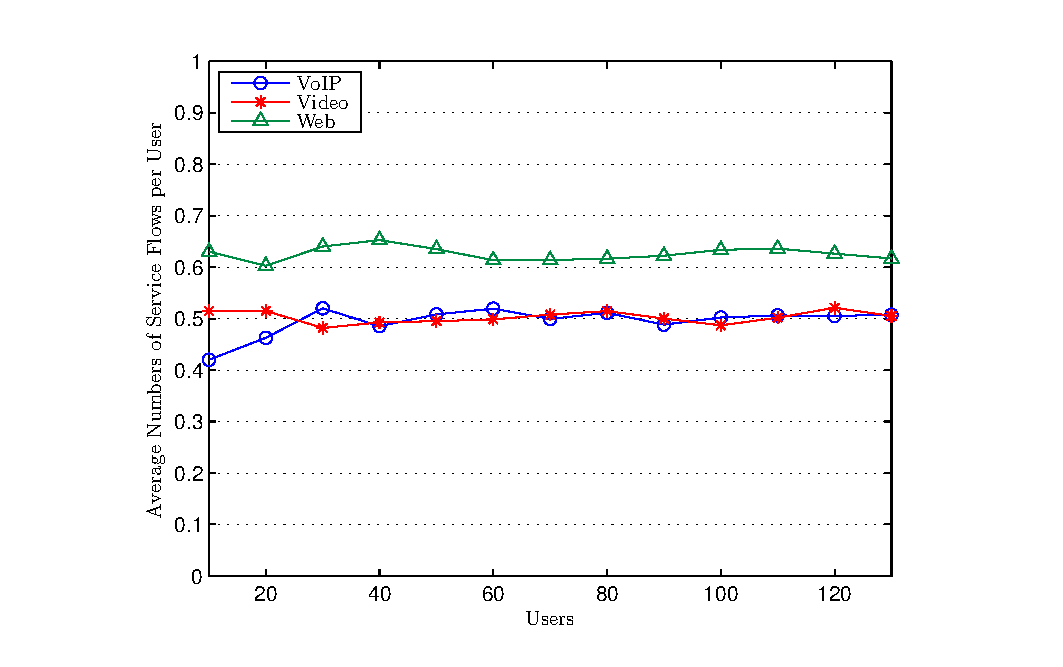
\includegraphics[%
  	scale=0.7,keepaspectratio]{figure/Flows/Flows_avg}
\caption{\label{fig:Flow_avg}隨機服務流數量下使用者裝置平均服務流數量圖。}
\end{figure}
\begin{figure}[H]
\centering
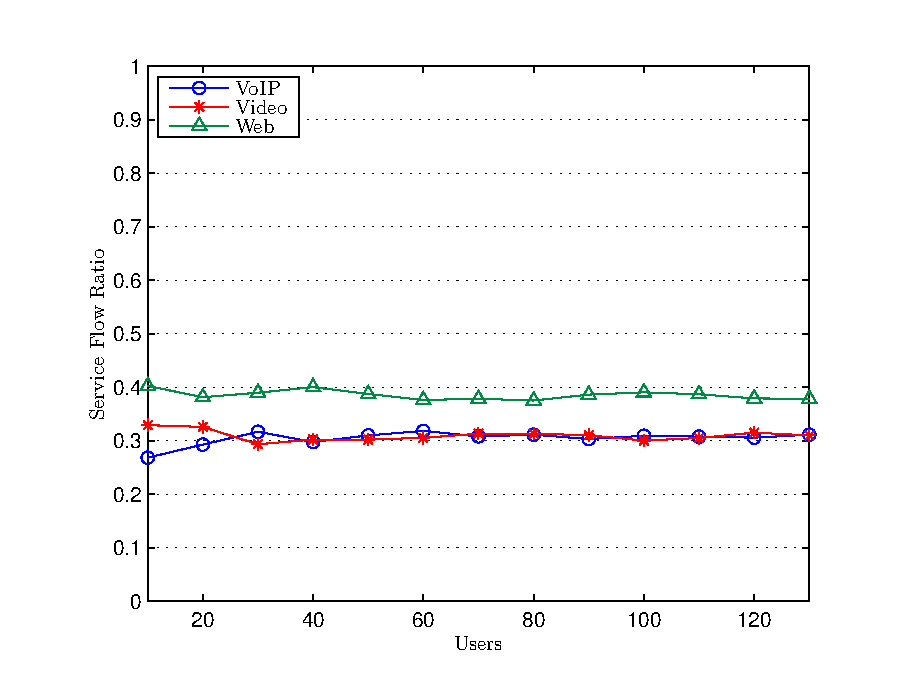
\includegraphics[%
  	scale=0.7,keepaspectratio]{figure/Flows/Flows_ratio}
\caption{\label{fig:Flow_ratio}隨機服務流數量下各服務流所佔比例圖。}
\end{figure}
\begin{figure}[H]
\centering
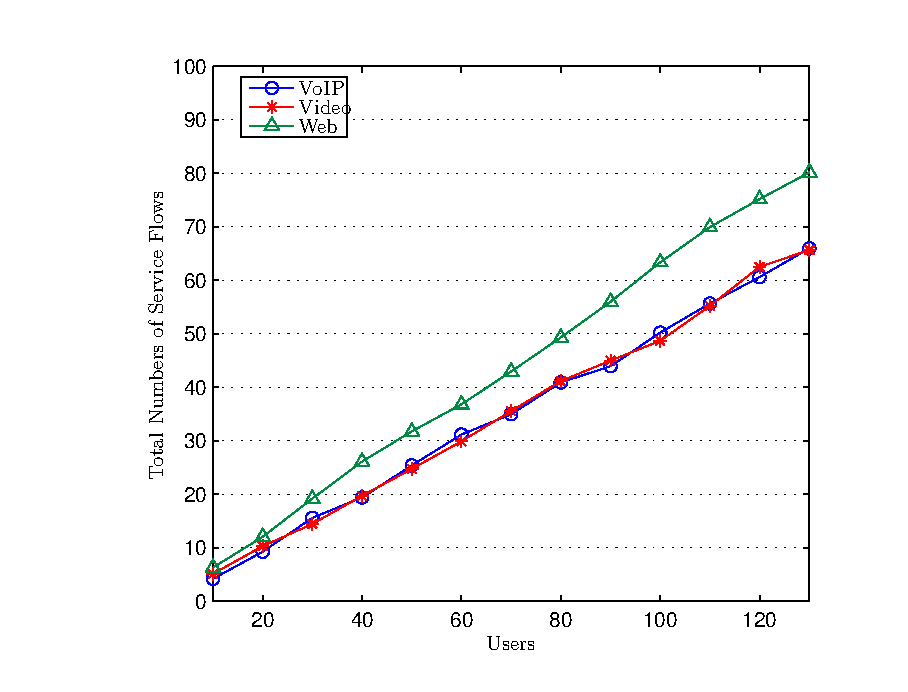
\includegraphics[%
  	scale=0.7,keepaspectratio]{figure/Flows/Flows_numbers}
\caption{\label{fig:Flow_numbers}隨機服務流數量下各服務流數量圖。}
\end{figure}
\end{comment}
\clearpage
\section{加權公平性}
在模擬環境中我們使用三種不同的服務流模擬資料傳輸的狀況,分別有兩種即時性與一種非即時性服務流,但是這三種服務流所能產生的吞吐量不同,在計算使用者裝置之間的公平性時需要給予其不同的權重。在固定的服務流數量下,每個使用者裝置在三種不同的服務流上都各自擁有同樣數量的服務流,在計算彼此之間的公平性時,每個使用者裝置不需要另外加上權重;而在隨機的服務流數量下,每個使用者裝置在三種服務流上所擁有的服務流數量不同,不同使用者裝置自身的吞吐量會產生差異,因此,由Jain等人所提出的普遍被使用於表示公平性的珍式公平性指標(Jain's Fairness Index)\cite{jain1984}僅適用於本碩士論文中使用的固定服務流數量模擬環境,而不完全適用於另外提出的隨機服務流數量模擬環境,珍式公平性指標的計算方式如公式(\ref{Jain})所示,其中$T_n$代表使用者裝置$n$的總吞吐量,$\mathcal{N}$為使用者裝置總數,
\begin{equation}
\label{Jain}
J=\dfrac{\Bigg[\sum\limits_{n=1}^\mathcal{N} T_n\Bigg]^2}{\mathcal{N}\times\Bigg[\sum\limits_{n=1}^\mathcal{N}{T_n}^2\Bigg]}
\end{equation}

而根據\cite{ferng2009},在計算公平性時,由於不同種類的服務流能產生的吞吐量並不相同,VoIP與Video服務流能產生的吞吐量便相差許多,因此,在計算兩者之間的公平性時必須要給予其不同的權重,再進行公平性的計算。於\cite{ferng2009}中提出三種不同層級觀察公平性時所使用的加權計算方式,分別為相同服務流之間、不同服務流之間與不同使用者裝置之間,其中不同使用者裝置之間對於使用者裝置$i$所使用的加權值$w_i$計算方式如公式(\ref{weight})所表示,
\begin{equation}
\label{weight}
w_i=\dfrac{\sum_l\sum_jK_{j,l}^i}{\sum_i\sum_l\sum_jK_{j,l}^i}
\end{equation}
其中$K_{j,l}^i$代表使用者裝置$i$中服務流種類$l$下的第$j$個服務流的期望吞吐量。在本碩士論文中,隨機服務流數量的環境下,每種服務流的數量最多只會有1個,最少為0個存在於使用者裝置內,因此,可以將公式(\ref{weight})改寫如下表示:
\begin{equation}
\label{simple_weight}
w_i=\dfrac{\sum_l\delta(i,l)K_l^i}{\sum_i\sum_l\delta(i,l)K_l^i}
\end{equation}
其中$K_l^i$代表使用者裝置$i$中服務流種類$l$的期望吞吐量,$\delta(i,l)$表示使用者裝置$i$中是否存在服務流種類$l$,如果使用者裝置$i$中存在服務流種類$l$,則$\delta(i,l)=1$,反之,則$\delta(i,l)=0$。透過公式(\ref{simple_weight})計算出$w_i$後,便可以將各使用者裝置的加權值$w_i$加入公式(\ref{Jain}),將其改寫成計算適用於評估本碩士論文中隨機服務流數量環境下$\mathcal{N}$個使用者裝置間的整體公平性$F_I$,其中的$T_i$為使用者裝置$i$模擬結果的實質吞吐量。
\begin{equation}
\label{fairness_index}
F_I=\dfrac{\Bigg[\sum\limits_{i=1}^\mathcal{N}\dfrac{T_i}{w_i}\Bigg]^2}{\mathcal{N}\times\Bigg[\sum\limits_{i=1}^\mathcal{N}\Big(\dfrac{T_i}{w_i}\Big)^2\Bigg]},
\quad 0\leq F_I\leq 1
\end{equation}

公平性$F_I$會是一個介於0與1之間的正數,$F_I$越靠近0則表示公平性越低落,使用者裝置之間加權過後的吞吐量差異越巨大,資源可能集中在部分使用者裝置上而可以有較多的吞吐量;若$F_I$越靠近1則可以說明使用者裝置之間的公平性越高,加權過後的吞吐量的差異並不多,使用者裝置都能獲得足夠的資源以傳輸資料。
\section{植基於急迫性之公平排程法分析}
我們所提出的排程演算法UFS主要考量使用者裝置的急迫度與平均配置資源度,同時在資源區塊的連續分配上加入調變編碼技術限制。將使用者裝置的急迫度、平均配置資源度與調變編碼技術限制這三種考量加入排程演算法的原因與希望達到的效果皆不相同,加入急迫度是希望能減少封包在佇列中因為超過延遲預算而被丟棄的機率,平均配置資源度則是用來增加過去拿到相對較少資源的使用者裝置能優先拿到資源的機率,最後,調變編碼技術限制讓連續分配時可以提高資源區塊的使用效率與更多使用者裝置可以分配到資源的機率。本節將比較UFS中所考量的急迫度、平均配置資源度與連續分配時的調變編碼技術限制各自帶來的影響,同時,討論在公式(\ref{Priority})中使用不同指數數值的$\mu$與$\nu$時,分別在端點對端點延遲、封包遺失率、公平性與吞吐量上的影響。
\clearpage
\subsection{優先權值指數選擇}
在UFS中,用於決定使用者裝置取得資源優先順序的公式(\ref{Priority})中,可以利用$\mu$與$\nu$分別調整急迫度$U_i(t)$與平均配置資源度$\overline{A_i(t)}$對優先權值$P_i(t)$的影響程度。在公式(\ref{Priority})中,急迫度$U_i(t)$做為主要影響優先權值$P_i(t)$的主要原因,平均配置資源度$\overline{A_i(t)}$則做為輔助急迫度的權值。為了進一步了解調整指數$\mu$與$\nu$對優先權值$P_i(t)$的影響,我們將使用以下不同的數值帶入公式(\ref{Priority})中:
\begin{equation}
\left . 
\begin{array}{l} 
\mu=1,\nu=0
 \\ 
\mu=0,\nu=1
 \\ 
\mu=1,\nu=1
 \\ 
\mu=0.5,\nu=1
 \\ 
\mu=1.5,\nu=0.5
\end{array}\right .
\end{equation}
在指數數值的選擇上,我們除了討論各自單獨使用急迫度或平均配置資源度決定使用者裝置分配資源的優先順序的情形外,我們也在$0\leq\mu\leq 2$與$0\leq\nu\leq 1$的範圍內討論幾組不同的數值,找出不同程度的急迫度與平均配置資源度影響使用者裝置優先順序的結果。我們可以透過圖 \ref{fig:UFS_delay_voip}、圖 \ref{fig:UFS_delay_video}、圖 \ref{fig:UFS_delay_web}、圖 \ref{fig:UFS_PLR}、圖 \ref{fig:UFS_Fairness}、圖 \ref{fig:UFS_Throughput}觀察使用不同的$\mu$與$\nu$調整急迫度$U_i(t)$與平均配置資源度$\overline{A_i(t)}$對優先權值$P_i(t)$在端點對端點延遲、封包遺失率、公平性與吞吐量上的影響。
\begin{comment}
\begin{figure}[H]
\centering
\subfigure[\label{fig:UFS_fix_delay}固定服務流數量UFS使用不同指數時的整體端點對端點延遲。]{
 	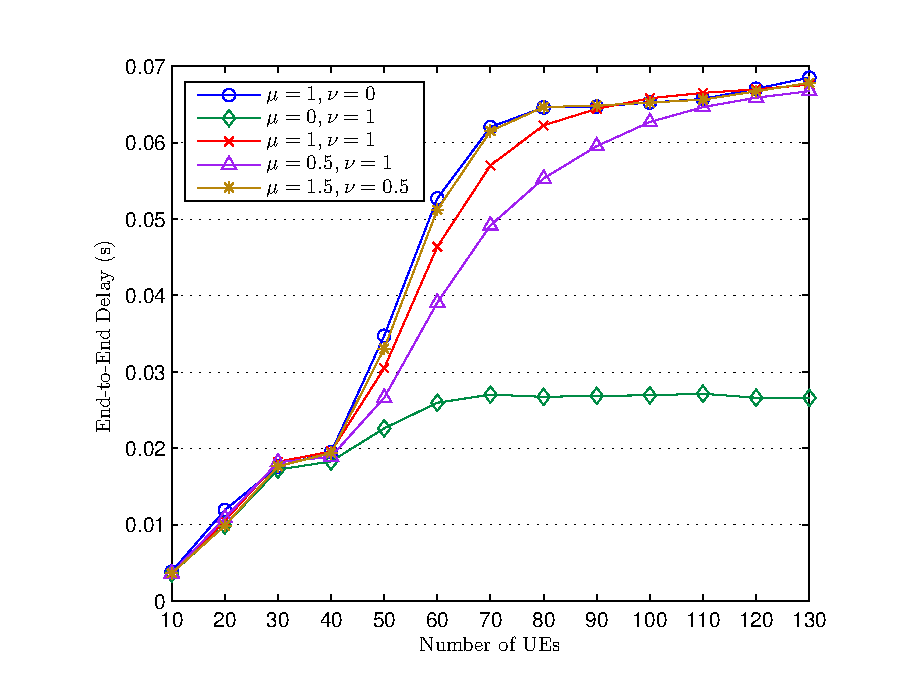
\includegraphics[%
  	scale=0.7,keepaspectratio]{figure/UFS/fixed/Delay}
}
\subfigure[\label{fig:UFS_ran_delay}隨機服務流數量UFS使用不同指數時的整體端點對端點延遲。]{
	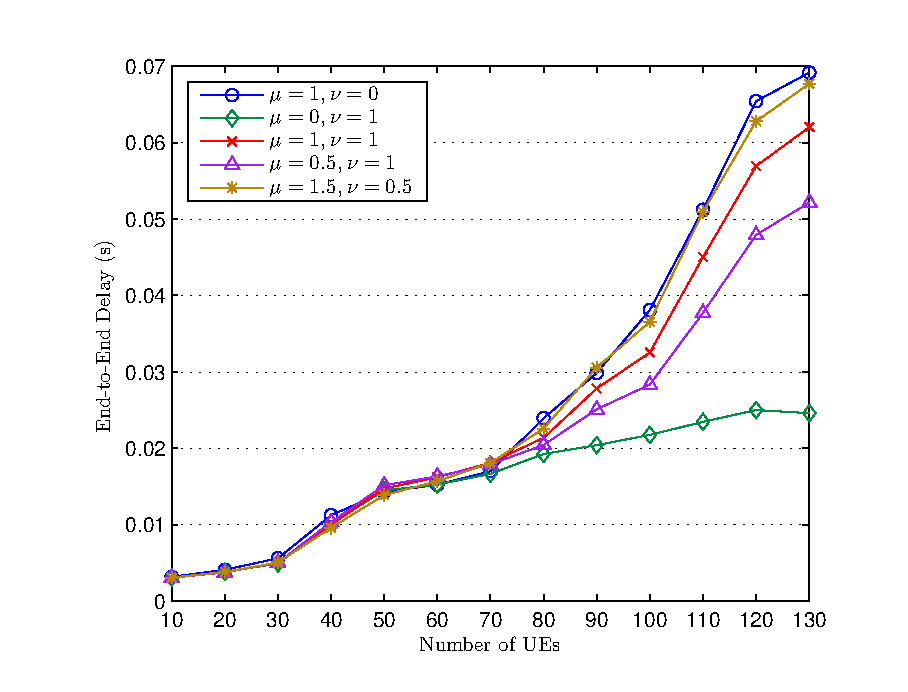
\includegraphics[%
	scale=0.7,keepaspectratio]{figure/UFS/random/Delay}
}
\caption{\label{fig:UFS_delay}不同環境中UFS使用不同指數時的整體端點對端點延遲。}
\end{figure}
\end{comment}
\begin{figure}[H]
\centering
\subfigure[\label{fig:UFS_fix_delay_voip}固定服務流數量下UFS使用不同指數時VoIP的端點對端點延遲。]{
 	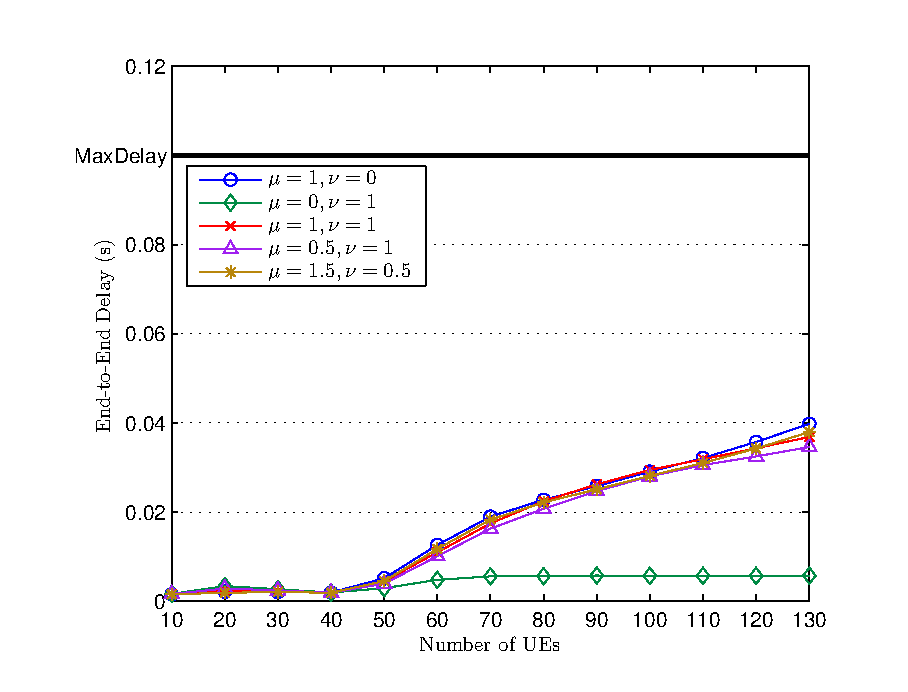
\includegraphics[%
  	scale=0.7,keepaspectratio]{figure/UFS/fixed/Delay_VoIP}
}
\subfigure[\label{fig:UFS_ran_delay_voip}隨機服務流數量下UFS使用不同指數時VoIP的端點對端點延遲。]{
	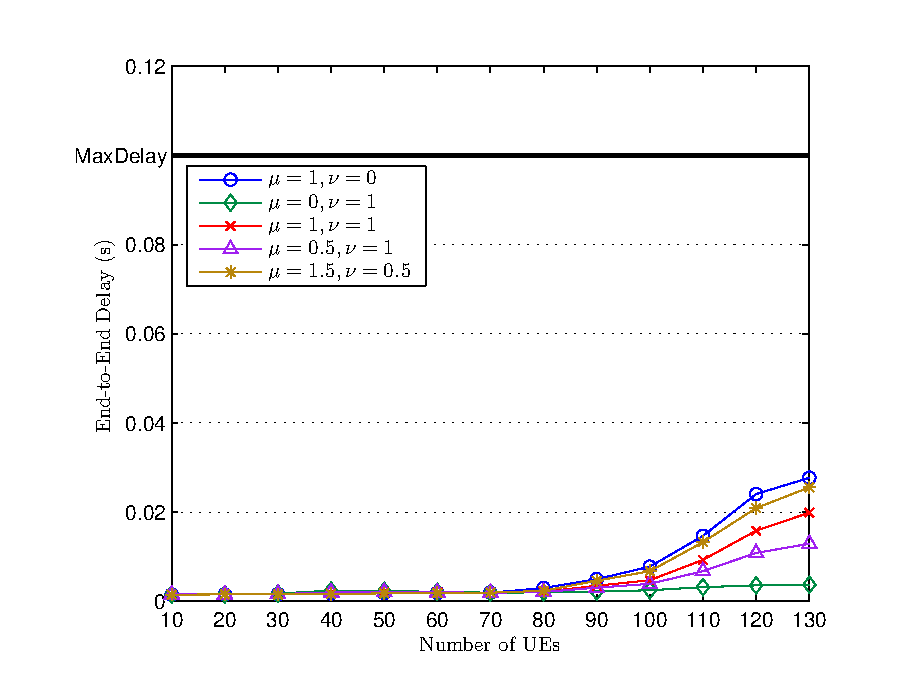
\includegraphics[%
	scale=0.7,keepaspectratio]{figure/UFS/random/Delay_VoIP}
}
\caption{\label{fig:UFS_delay_voip}不同環境中UFS使用不同指數時VoIP服務流的端點對端點延遲。}
\end{figure}
\begin{figure}[H]
\centering
\subfigure[\label{fig:UFS_fix_delay_video}固定服務流數量下UFS使用不同指數時Video的端點對端點延遲。]{
 	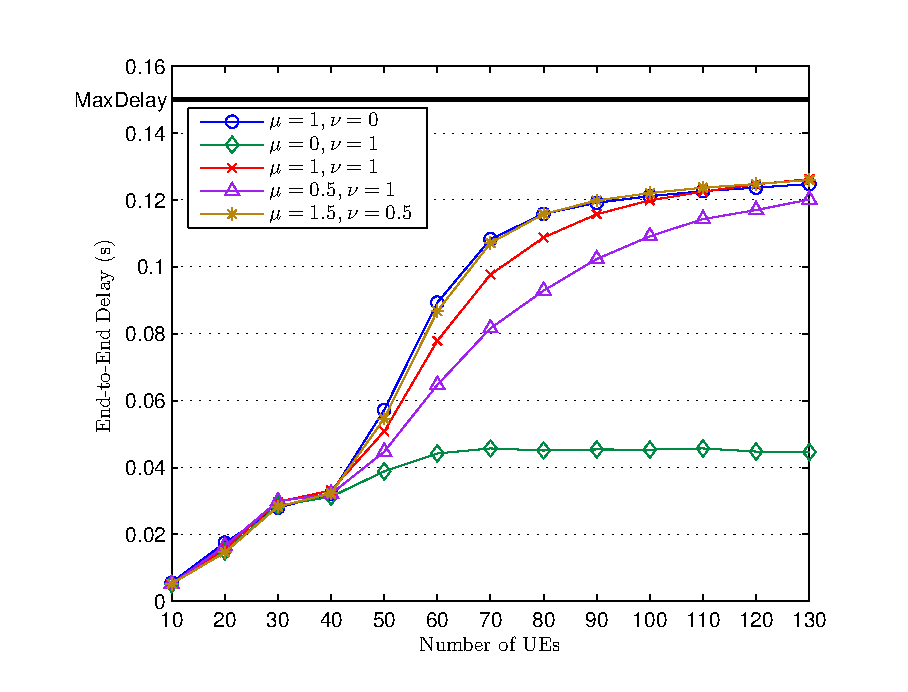
\includegraphics[%
  	scale=0.7,keepaspectratio]{figure/UFS/fixed/Delay_Video}
}
\subfigure[\label{fig:UFS_ran_delay_video}隨機服務流數量下UFS使用不同指數時Video的端點對端點延遲。]{
	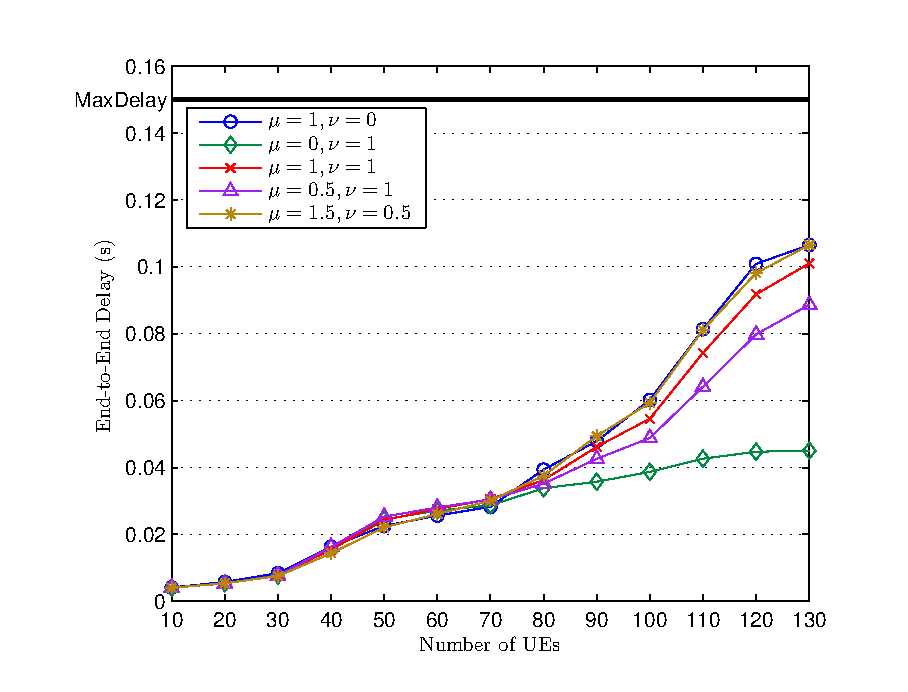
\includegraphics[%
	scale=0.7,keepaspectratio]{figure/UFS/random/Delay_Video}
}
\caption{\label{fig:UFS_delay_video}不同環境中UFS使用不同指數時Video服務流的端點對端點延遲。}
\end{figure}
\begin{figure}[H]
\centering
\subfigure[\label{fig:UFS_fix_delay_web}固定服務流數量下UFS使用不同指數時Web的端點對端點延遲。]{
 	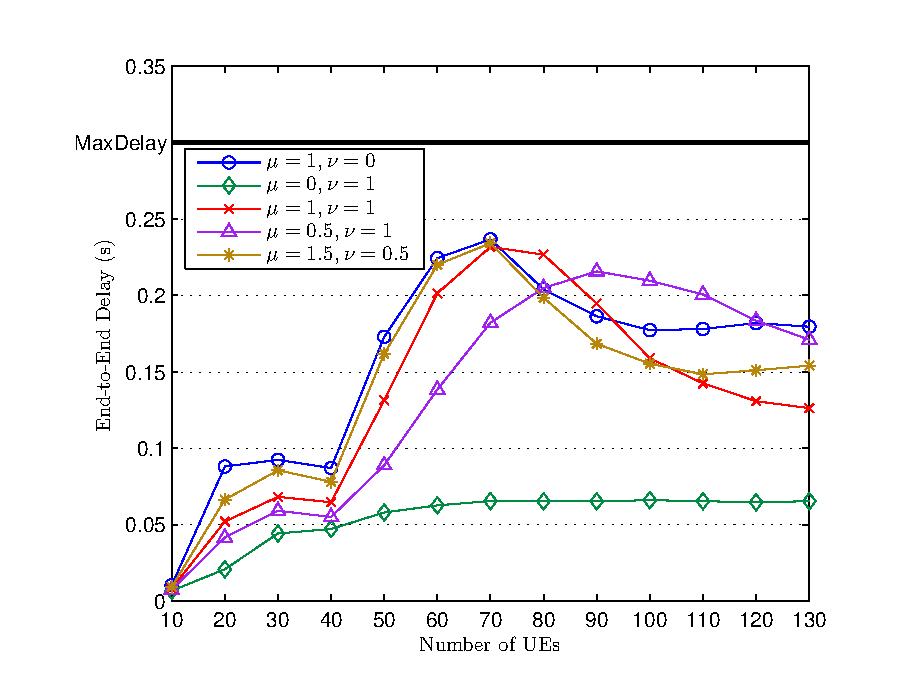
\includegraphics[%
  	scale=0.7,keepaspectratio]{figure/UFS/fixed/Delay_Web}
}
\subfigure[\label{fig:UFS_ran_delay_web}隨機服務流數量下UFS使用不同指數時Web的端點對端點延遲。]{
 	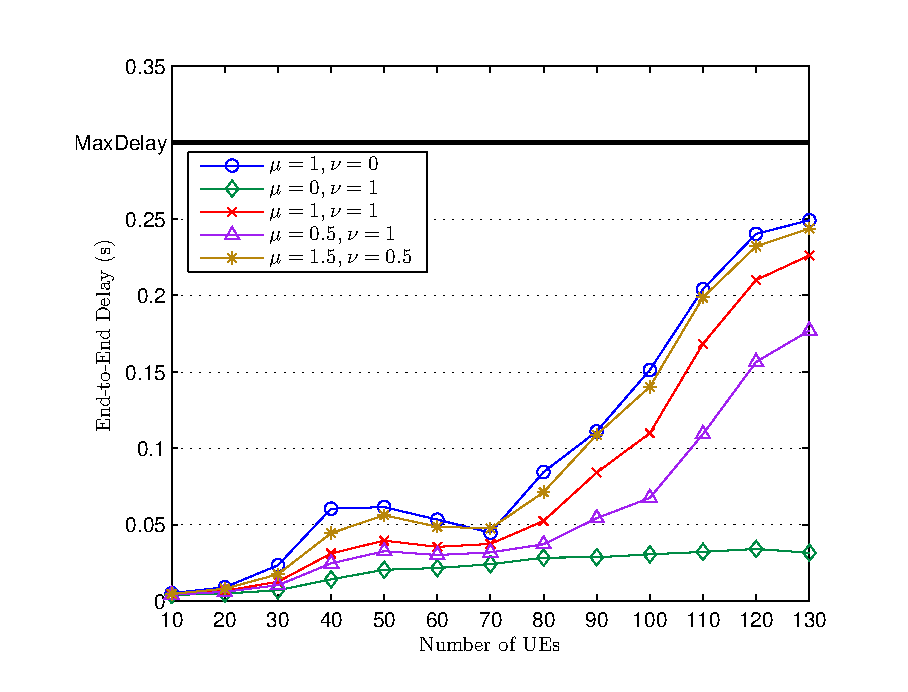
\includegraphics[%
  	scale=0.7,keepaspectratio]{figure/UFS/random/Delay_Web}
}
\caption{\label{fig:UFS_delay_web}不同環境中UFS使用不同指數時Web服務流的端點對端點延遲。}
\end{figure}
圖 \ref{fig:UFS_delay_voip}、圖 \ref{fig:UFS_delay_video}、圖 \ref{fig:UFS_delay_web}分別為不同環境下UFS使用不同指數時對各服務流的端點對端點延遲影響,可以發現當$\mu=1,\nu=0$時會有最高的端點對端點延遲,原因在於此時使用者裝置取得資源的優先順序完全由急迫度$U_i(t)$控制,使用者裝置只有在服務流延遲預算剩餘時間越來越少時才有機會優先取得資源,因此,封包在佇列中的延遲時間便會增加;當$\mu=0,\nu=1$時,各服務流的端點對端點延遲時間都會是最低的,此時使用者裝置取得資源的優先順序則是由平均配置資源度$\overline{A_i(t)}$決定,封包在佇列中的延遲預算剩餘時間不影響優先權值$P_i(t)$,因此,在使用者裝置佇列中的封包不會被迫等待至接近延遲預算上限才得到資源,各服務流佇列中的封包延遲時間減少。
\begin{figure}[H]
\centering
\subfigure[\label{fig:UFS_fix_PLR}固定服務流數量下UFS使用不同指數時的封包遺失率。]{
 	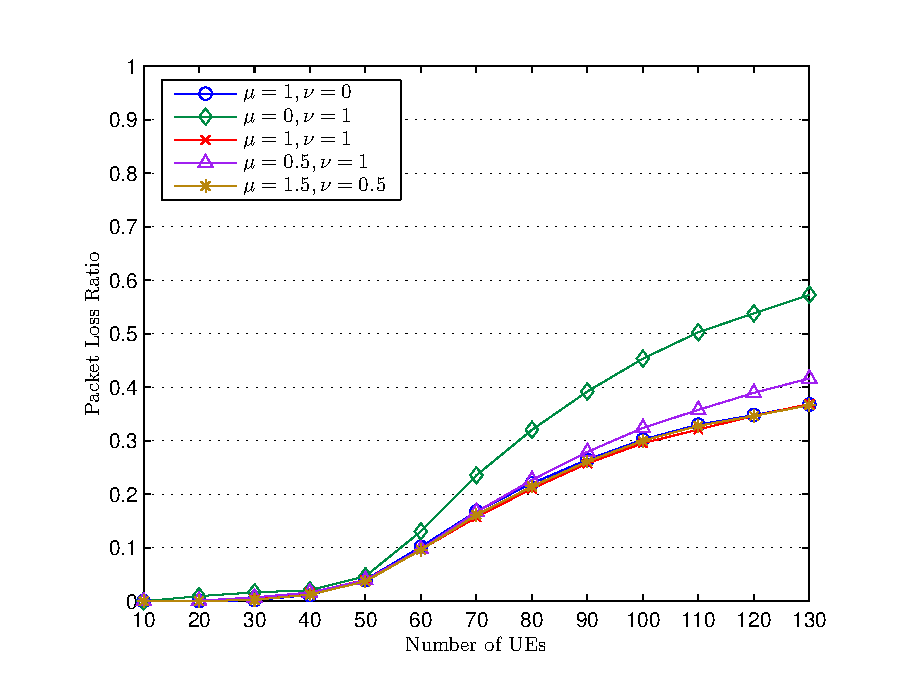
\includegraphics[%
  	scale=0.7,keepaspectratio]{figure/UFS/fixed/PLR}
}
\subfigure[\label{fig:UFS_ran_PLR}隨機服務流數量下UFS使用不同指數時的封包遺失率。]{
	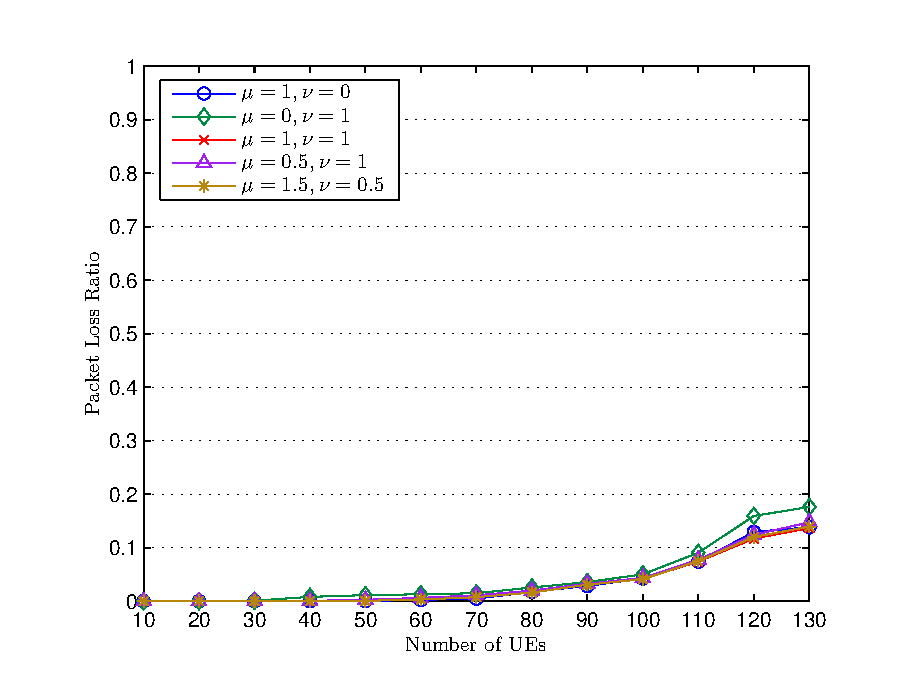
\includegraphics[%
	scale=0.7,keepaspectratio]{figure/UFS/random/PLR}
}
\caption{\label{fig:UFS_PLR}不同環境中UFS使用不同指數時的封包遺失率。}
\end{figure}
圖 \ref{fig:UFS_PLR}為不同環境下UFS使用不同指數時對封包遺失率的影響。當$\mu=0,\nu=1$時,在兩種不同環境都會有最高的封包遺失率,因為其並不考慮使用者裝置內佇列中封包的延遲情形,封包遺失率會高於其他$\mu > 0$考慮使用者裝置急迫度時的情況;當$\mu=0.5,\mu=1,\mu=1.5$時,不論是否$\nu>0$或是$\nu=0$,都能有較低的封包遺失率,同時,彼此之間的差距微小,因為考量了使用者裝置的急迫度,佇列中的封包在超過延遲預算之前使用者裝置便有機會取得資源,封包在佇列中超過延遲預算被丟棄的機率下降。
\begin{figure}[H]
\centering
\subfigure[\label{fig:UFS_fix_fairness}固定服務流數量下UFS使用不同指數時的公平性。]{
 	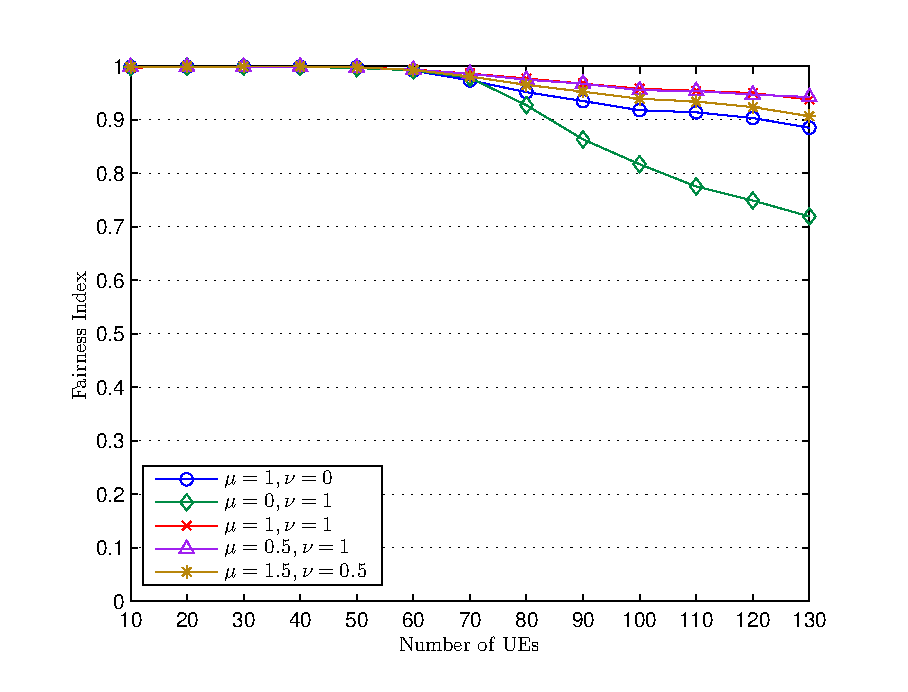
\includegraphics[%
  	scale=0.7,keepaspectratio]{figure/UFS/fixed/Fairness}
}
\subfigure[\label{fig:UFS_ran_fairness}隨機服務流數量下UFS使用不同指數時的公平性。]{
	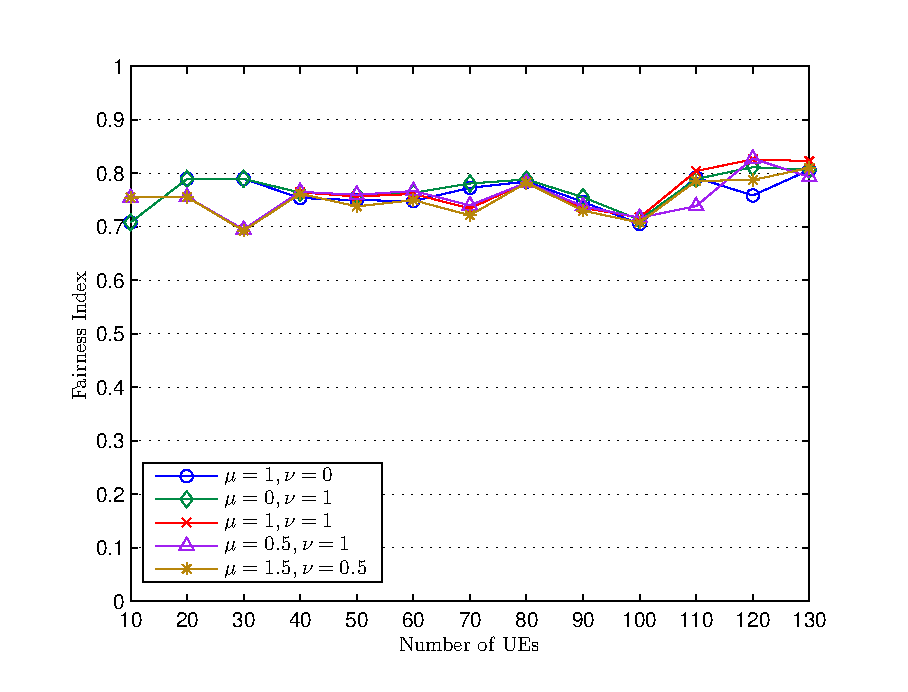
\includegraphics[%
	scale=0.7,keepaspectratio]{figure/UFS/random/Fairness}
}
\caption{\label{fig:UFS_Fairness}不同環境中UFS使用不同指數時的公平性。}
\end{figure}
圖 \ref{fig:UFS_Fairness}為不同環境下UFS使用不同指數時對公平性的影響。在圖 \ref{fig:UFS_fix_fairness}中,當$\mu=0,\nu=1$時整體的公平性最低,因為只以平均配置資源度決定使用者裝置取得資源的優先順序,較高的封包遺失率讓整體公平性下降;從$\mu=1,\nu=0$與$\mu=1,\nu=1$的結果可以發現,僅考量使用者裝置的急迫度時,整體的公平性已經有不錯的表現,但是,將平均配置資源度加入調整優先權值後,可以有更佳的整體公平性。
\begin{figure}[H]
\centering
\subfigure[\label{fig:UFS_fix_Throughput}固定服務流數量下UFS使用不同指數時的吞吐量。]{
 	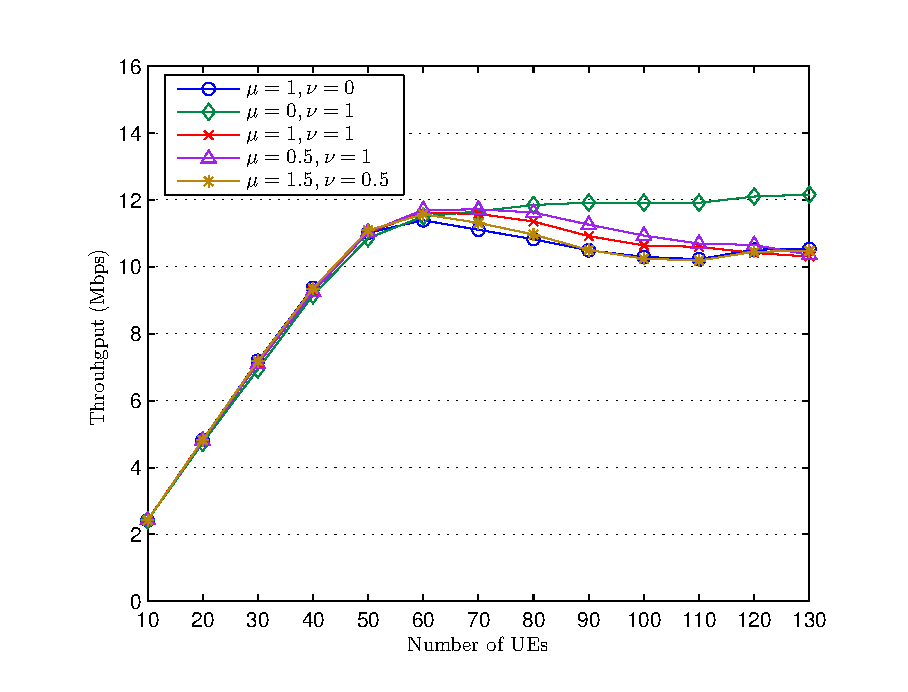
\includegraphics[%
  	scale=0.7,keepaspectratio]{figure/UFS/fixed/Throughput}
}
\subfigure[\label{fig:UFS_ran_Throughput}隨機服務流數量下UFS使用不同指數時的吞吐量。]{
	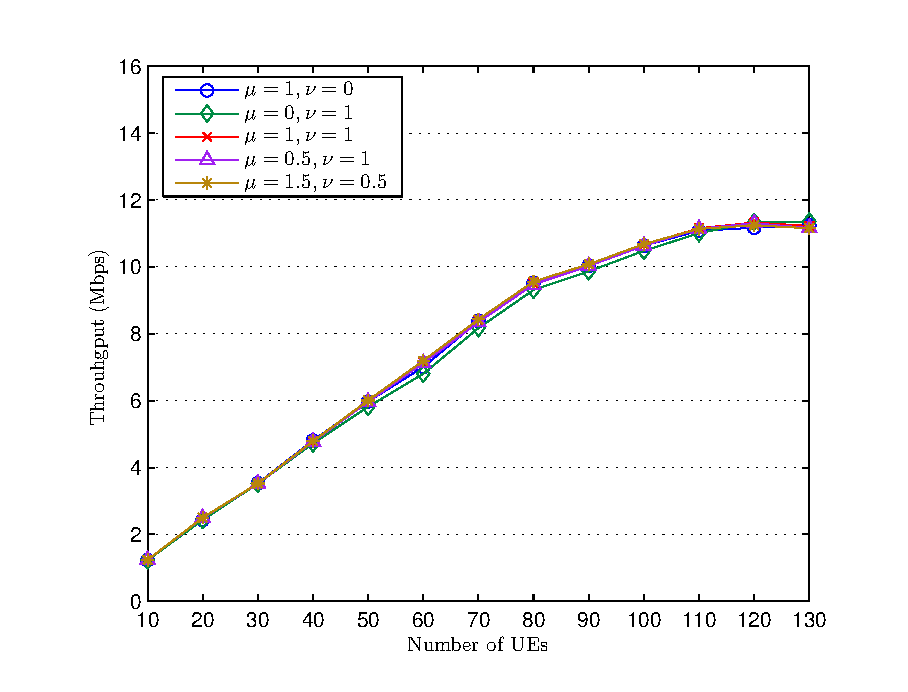
\includegraphics[%
	scale=0.7,keepaspectratio]{figure/UFS/random/Throughput}
}
\caption{\label{fig:UFS_Throughput}不同環境中UFS使用不同指數時的吞吐量。}
\end{figure}
圖 \ref{fig:UFS_Throughput}為不同環境下UFS使用不同指數時對吞吐量的影響。在圖 \ref{fig:UFS_fix_Throughput}中可以發現,當$\mu=0,\nu=1$時系統的吞吐量比其他情況都高,原因在於固定服務流數量時,使用者裝置中的服務流種類和數量固定,造成當$\mu>0$將使用者裝置急迫度加入優先權值的考量時,使用者裝置之間的急迫度差異不大,使UFS的循環性程度上升,整體的吞吐量下降;在隨機服務流數量時,使用者裝置之間的服務流種類與數量皆不盡相同,急迫度的差異性明顯,資源分配上可以得到更高的效果。

透過圖 \ref{fig:UFS_delay_voip}、圖 \ref{fig:UFS_delay_video}、圖 \ref{fig:UFS_delay_web}、圖 \ref{fig:UFS_PLR}、圖 \ref{fig:UFS_Fairness}、圖 \ref{fig:UFS_Throughput},我們可以發現,調整UFS中急迫度$U_i(t)$與平均配置資源度$\overline{A_i(t)}$的指數$\mu,\nu$,可以改變急迫度與平均配置資源度在不同評估結果上的影響。在$1 \leq \mu \leq \mu_{MAX}$的範圍中,當$\mu$越大時,急迫度對優先順序的影響程度上升,封包預算剩餘時間越短的使用者裝置即使配置過較多的資源區塊,仍然會比其他使用者裝置容易得到資源,可以減少封包在佇列中被丟棄的機率,降低整體的封包遺失率;在$0 \leq \nu \leq 1$的範圍中,當$\nu$越大時,平均配置資源度的影響上升,在端點對端點延遲上可以有較低的延遲。我們可以針對想要提升的特定效果,選擇不同的指數來調整急迫度與平均配置資源度對優先權值的影響;我們同時也可以發現,平均配置資源度對優先順序的影響程度並不如急迫度,主要用於輔助調整優先權值,同時,當$\mu=1,\nu=1$時,從各項較能評估結果綜合來看,可以取得較好的效果,因此,在本章節之後用於比較各方法之間的效能評估時,UFS皆使用$\mu=1,\nu=1$做為公式(\ref{Priority})中的指數數值,與其他方法在不同方面上的評估進行比較。

\subsection{調變編碼技術限制效果}
排程演算法在資源區塊的連續分配的方式上有各種不同的設計,一般的排程演算法利用通道品質決定連續分配的方式,而UFS則是使用調變編碼技術限制來決定分配給使用者裝置的資源區塊數量。UFS在資源連續分配的階段時,會依照公式(\ref{Threshold})判斷此次的排程是否使用調變編碼技術限制,滿足公式(\ref{Threshold})則會啟用限制並檢查分配該資源區塊是否會影響原先可以使用的調變編碼技術,若會造成原本可使用的調變等級下降,則不分配該資源區塊給使用者裝置,接著對下一個優先順序的使用者裝置開始分配資源。為能了解在資源區塊連續分配時使用調變編碼技術限制的影響,我們比較UFS在第一階段決定使用者裝置的分配資源優先順序後,於第二階段的資源區塊連續分配的方式上,使用調變編碼技術限制資源區塊數量(MCS-Constraint Sequential Allocation)以及分配固定資源區塊數量(Fixed Amount Sequential Allocation)兩種不同的連續分配方式,觀察在各服務流的端點對端點延遲、封包遺失率、公平性與吞吐量上的結果。
\begin{comment}
\begin{figure}[H]
\centering
\subfigure[\label{fig:MCS_fix_delay}固定服務流數量使用不同連續分配方式時的整體端點對端點延遲。]{
 	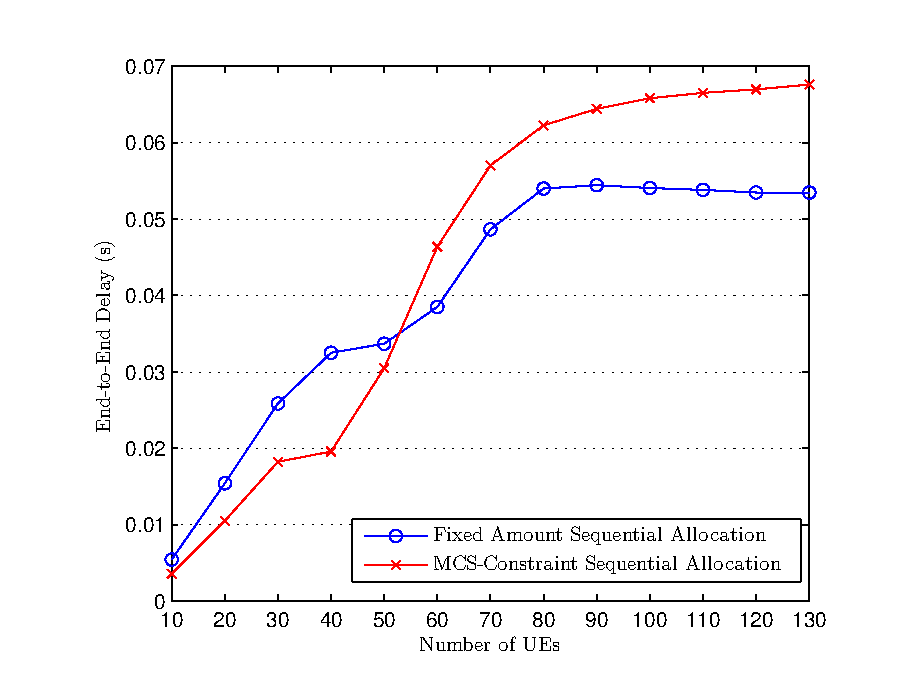
\includegraphics[%
  	scale=0.7,keepaspectratio]{figure/MCS/fixed/Delay}
}
\subfigure[\label{fig:MCS_ran_delay}隨機服務流數量使用不同連續分配方式時的整體端點對端點延遲。]{
	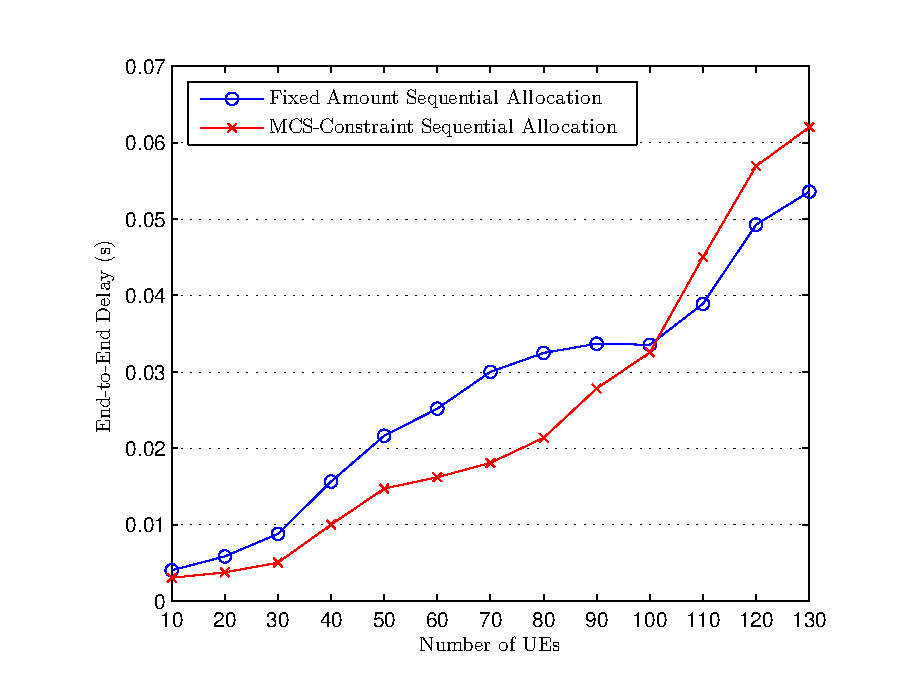
\includegraphics[%
	scale=0.7,keepaspectratio]{figure/MCS/random/Delay}
}
\caption{\label{fig:MCS_delay}不同環境中UFS使用不同連續分配方式時的端點對端點延遲。}
\end{figure}
\end{comment}
\begin{figure}[H]
\centering
\subfigure[\label{fig:MCS_fix_delay_voip}固定服務流數量下使用不同連續分配方式時VoIP的端點對端點延遲。]{
 	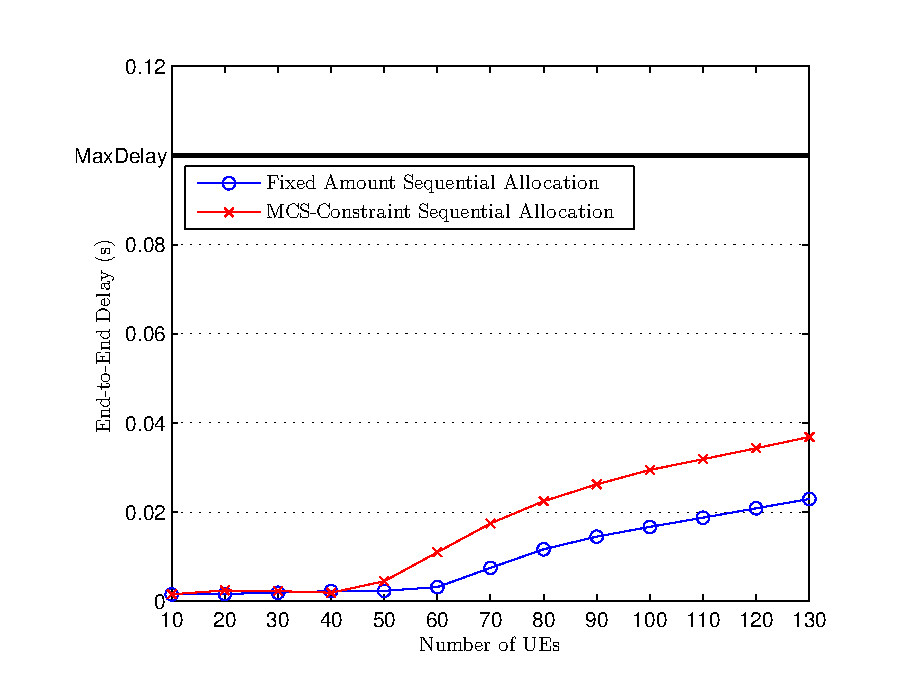
\includegraphics[%
  	scale=0.7,keepaspectratio]{figure/MCS/fixed/Delay_VoIP}
}
\subfigure[\label{fig:MCS_ran_delay_voip}隨機服務流數量下使用不同連續分配方式時VoIP的端點對端點延遲。]{
	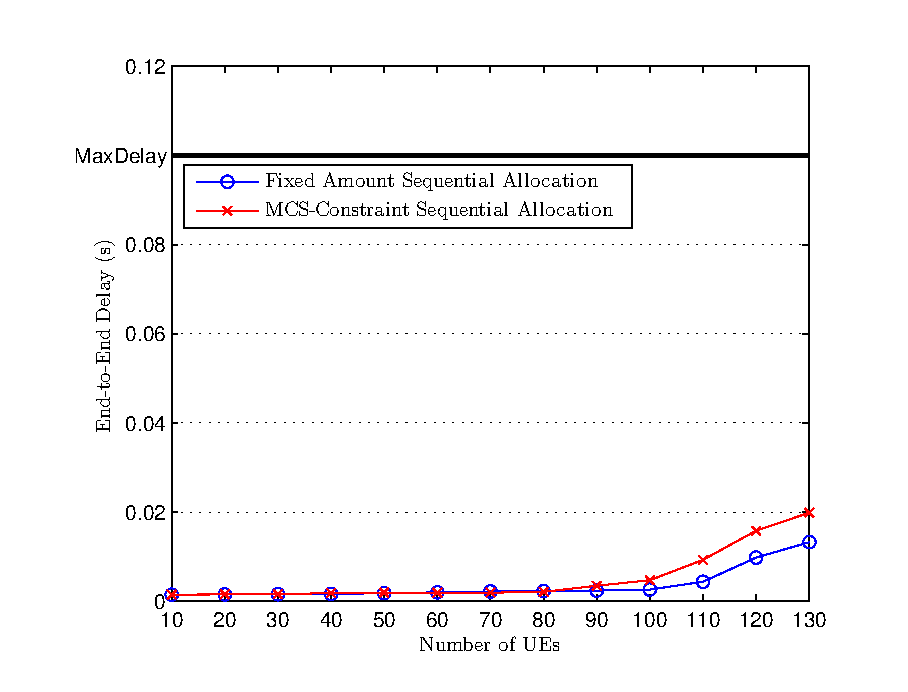
\includegraphics[%
	scale=0.7,keepaspectratio]{figure/MCS/random/Delay_VoIP}
}
\caption{\label{fig:MCS_delay_voip}不同環境中UFS使用不同連續分配方式時VoIP服務流的端點對端點延遲。}
\end{figure}
\begin{figure}[H]
\centering
\subfigure[\label{fig:MCS_fix_delay_video}固定服務流數量下使用不同連續分配方式時Video的端點對端點延遲。]{
 	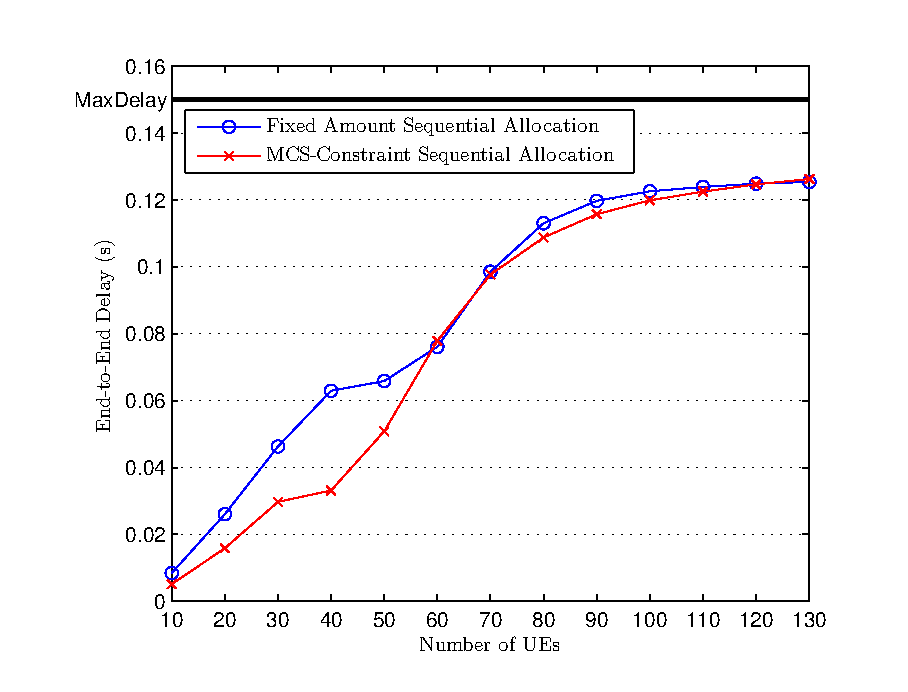
\includegraphics[%
  	scale=0.7,keepaspectratio]{figure/MCS/fixed/Delay_Video}
}
\subfigure[\label{fig:MCS_ran_delay_video}隨機服務流數量下使用不同連續分配方式時Video的端點對端點延遲。]{
	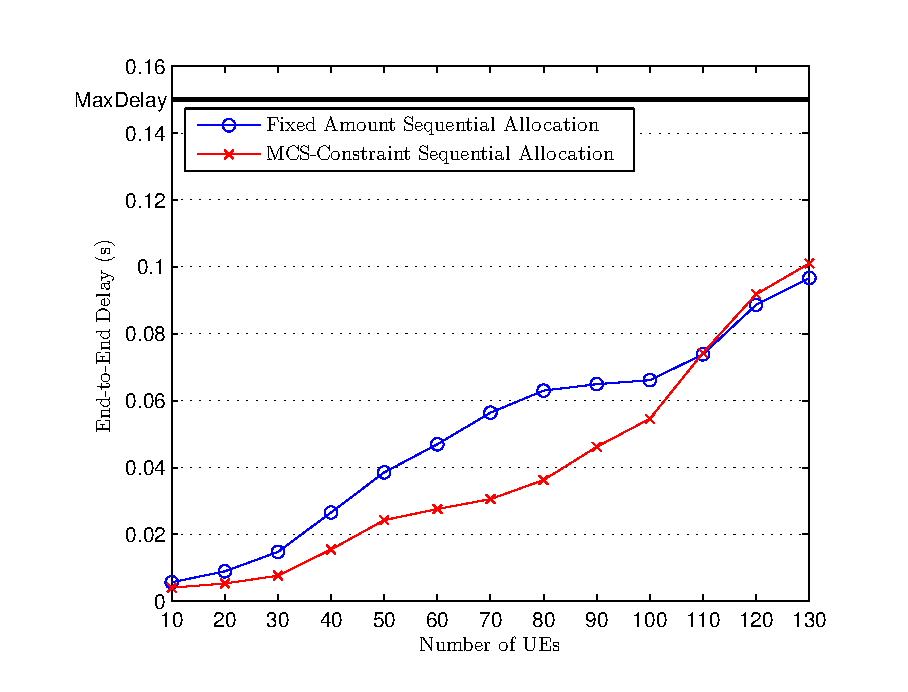
\includegraphics[%
	scale=0.7,keepaspectratio]{figure/MCS/random/Delay_Video}
}
\caption{\label{fig:MCS_delay_video}不同環境中UFS使用不同連續分配方式時Video服務流的端點對端點延遲。}
\end{figure}
\begin{figure}[H]
\centering
\subfigure[\label{fig:MCS_fix_delay_web}固定服務流數量下使用不同連續分配方式時Web的端點對端點延遲。]{
 	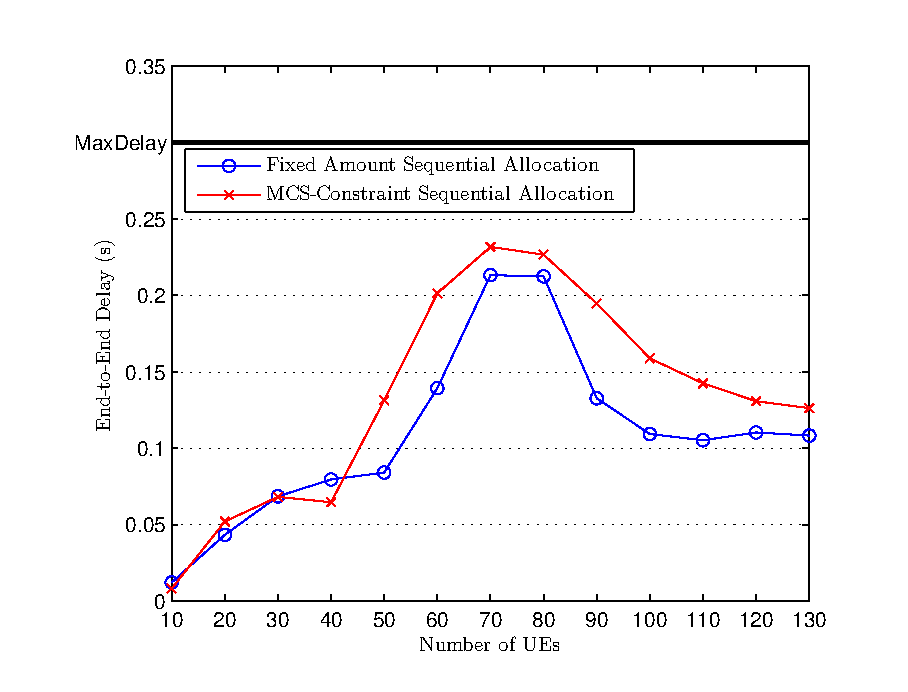
\includegraphics[%
  	scale=0.7,keepaspectratio]{figure/MCS/fixed/Delay_Web}
}
\subfigure[\label{fig:MCS_ran_delay_web}隨機服務流數量下使用不同連續分配方式時Web的端點對端點延遲。]{
 	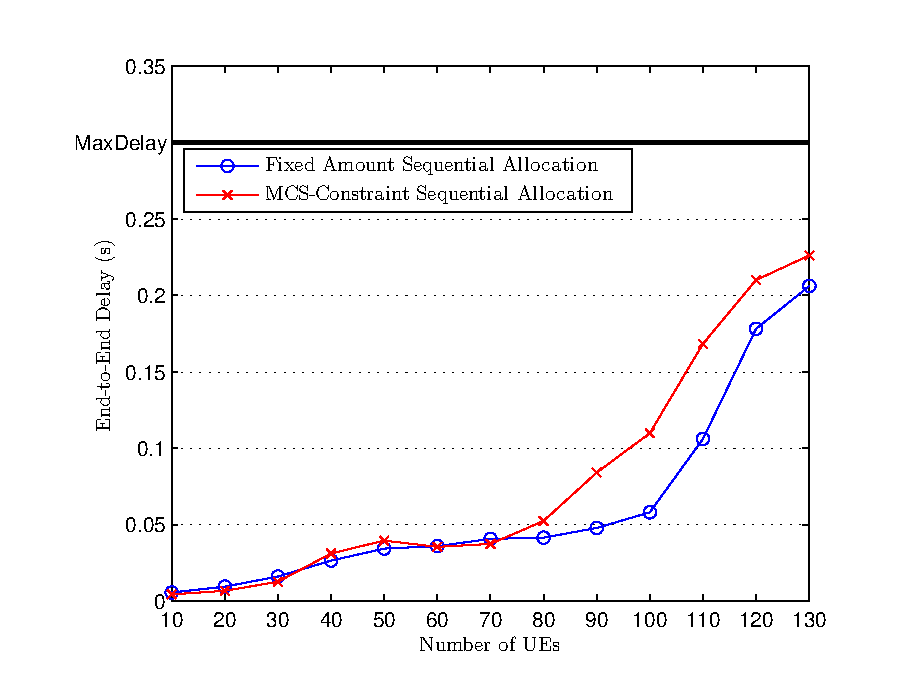
\includegraphics[%
  	scale=0.7,keepaspectratio]{figure/MCS/random/Delay_Web}
}
\caption{\label{fig:MCS_delay_web}不同環境中UFS使用不同連續分配方式時Web服務流的端點對端點延遲。}
\end{figure}
圖 \ref{fig:MCS_delay_voip}、圖 \ref{fig:MCS_delay_video}、圖 \ref{fig:MCS_delay_web}分別為使用不同的連續分配方式對各服務流的端點對端點延遲影響。我們可以發現使用調變編碼技術限制的連續分配方式在VoIP服務流會明顯有較高的延遲,Video服務流與Web服務流在較多使用者裝置時的延遲也會高於固定數量的連續分配方式,主要因為使用調變編碼技術限制時,排程器為了資源區塊能使用較高等級的調變技術,會限制使用者裝置可以取得的資源區塊數量,使用者裝置可能無法取得足夠的資源區塊傳輸佇列中的資料,使得封包在佇列中的等待時間變長,端點對端點延遲同時跟著增加;固定數量的連續分配方式在每次分配資源時會先根據使用者裝置的數量與可使用的資源區塊數量,決定平均一個使用者裝置可以取得的資源區塊數量,再依據優先順序依序分配連續的資源區塊給使用者裝置,因此,相較於使用調變編碼技術限制的連續分配方式,在單次的排程中使用者裝置可以取得較多資源區塊,可以傳輸佇列中的資料,減少封包在佇列中的延遲時間。

\begin{figure}[H]
\centering
\subfigure[\label{fig:MCS_fix_PLR}固定服務流數量下使用不同連續分配方式時的封包遺失率。]{
 	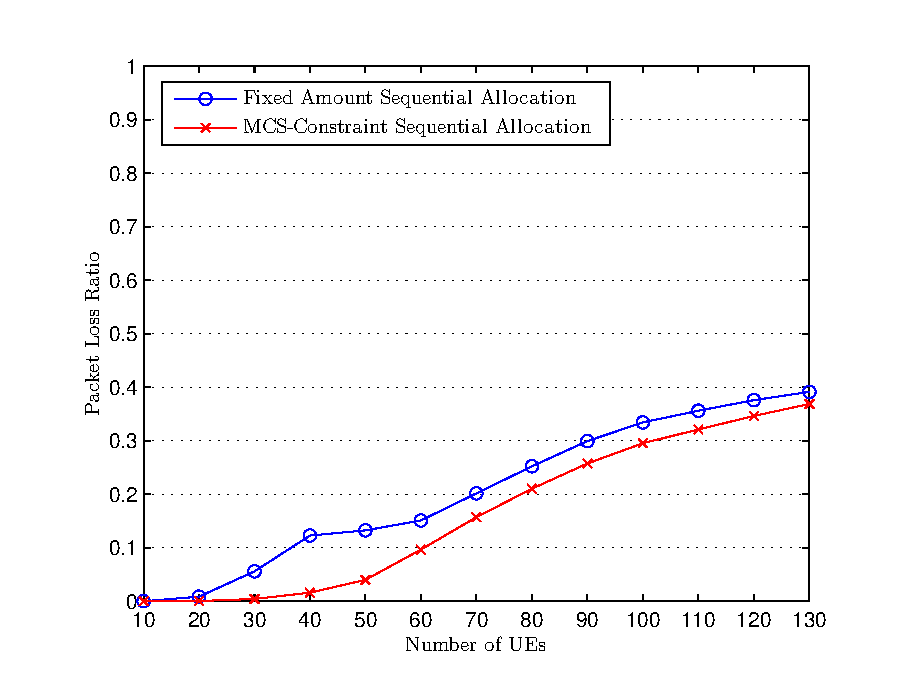
\includegraphics[%
  	scale=0.7,keepaspectratio]{figure/MCS/fixed/PLR}
}
\subfigure[\label{fig:MCS_ran_PLR}隨機服務流數量下使用不同連續分配方式時的封包遺失率。]{
	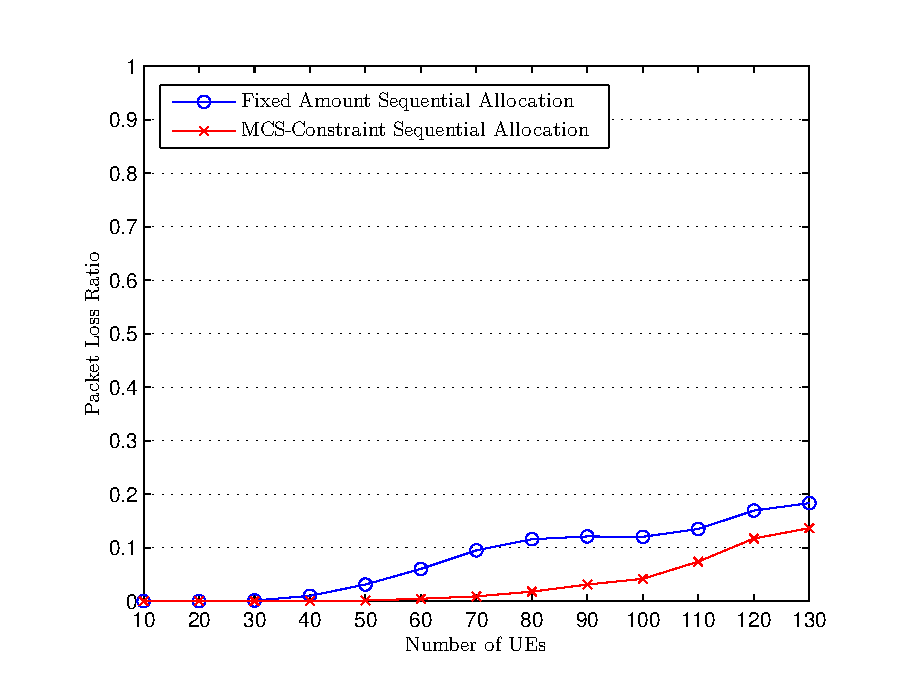
\includegraphics[%
	scale=0.7,keepaspectratio]{figure/MCS/random/PLR}
}
\caption{\label{fig:MCS_PLR}不同環境中UFS使用不同連續分配方式時的封包遺失率。}
\end{figure}
\begin{figure}[H]
\centering
\subfigure[\label{fig:MCS_fix_fairness}固定服務流數量下使用不同連續分配方式時的公平性。]{
 	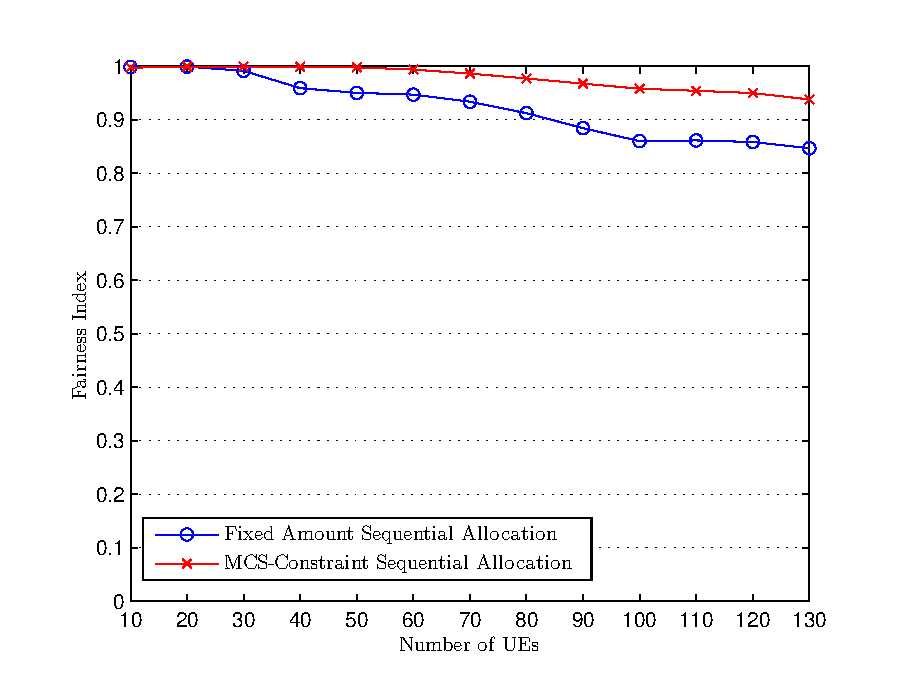
\includegraphics[%
  	scale=0.7,keepaspectratio]{figure/MCS/fixed/Fairness}
}
\subfigure[\label{fig:MCS_ran_fairness}隨機服務流數量下使用不同連續分配方式時的公平性。]{
	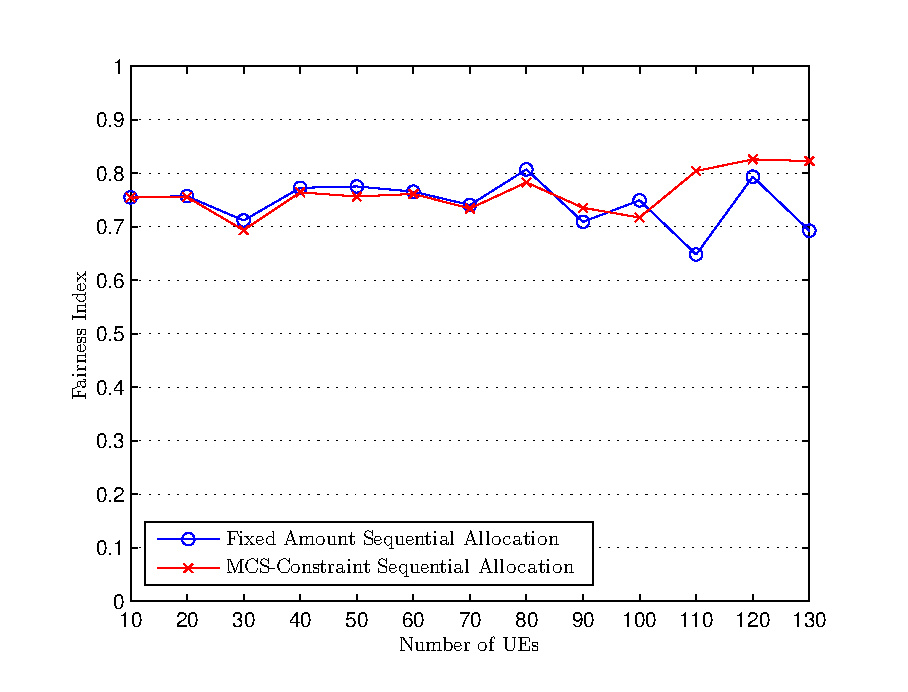
\includegraphics[%
	scale=0.7,keepaspectratio]{figure/MCS/random/Fairness}
}
\caption{\label{fig:MCS_Fairness}不同環境中UFS使用不同連續分配方式時的公平性。}
\end{figure}
\begin{figure}[H]
\centering
\subfigure[\label{fig:MCS_fix_Throughput}固定服務流數量下使用不同連續分配方式時的吞吐量。]{
 	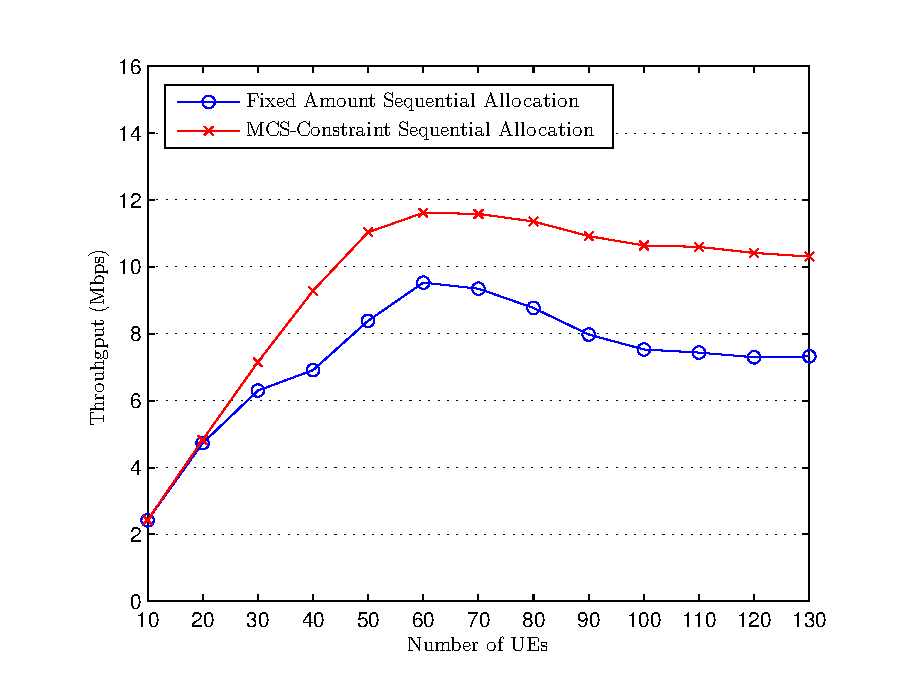
\includegraphics[%
  	scale=0.7,keepaspectratio]{figure/MCS/fixed/Throughput}
}
\subfigure[\label{fig:MCS_ran_Throughput}隨機服務流數量下使用不同連續分配方式時的吞吐量。]{
	\includegraphics[%
	scale=0.7,keepaspectratio]{figure/MCS/random/Throughput}
}
\caption{\label{fig:MCS_Throughput}不同環境中UFS使用不同連續分配方式時的吞吐量。}
\end{figure}
圖 \ref{fig:MCS_PLR}、圖 \ref{fig:MCS_Fairness}、圖 \ref{fig:MCS_Throughput}分別為使用不同的連續分配方式對整體的封包遺失率、公平性與吞吐量的影響。在資源區塊的連續分配上使用調變編碼技術限制時,這三種結果上都可以比固定數量的連續分配方式有更好的效果,主要原因在於,雖然調變編碼技術限制有機率會讓使用者裝置可以取得的資源區塊數量下降,但是,在單次的排程時會有更多使用者裝置可以取得資源區塊傳輸在佇列中等待的封包,降低封包遺失率以及提升使用者裝置之間的公平性;同時,調變編碼技術限制最主要的目的在維持資源區塊能使用的調變技術等級,提升資源區塊的資料傳輸效率,讓整體的吞吐量上升。綜合上述對連續分配方式的討論,在資源區塊的連續分配上使用調變編碼技術限制時,雖然在較多使用者裝置的環境時比固定數量的連續分配方式有更高的端點對端點延遲,但是,在封包遺失率、公平性與吞吐量上都會有較好的效果。

\section{各機制之端點對端點延遲}
端點對端點延遲為封包在佇列中的等待時間加上傳輸時間所得到的延遲時間,端點對端點延遲數值越高,表示封包從進入使用者裝置中的媒體存取控制層佇列開始,到抵達基地台中間的這段時間越長,對延遲敏感的服務流造成的影響越大;反之,端點對端點延遲數值越低,則延遲敏感的服務流能提供較佳的服務品質。我們所提出的UFS將使用者裝置內服務流的平均延遲預算剩餘時間定義為急迫度,並將其加入排程演算法,做為分配資源時決策使用者裝置優先程度的依據之一,目的在於拯救佇列頭端封包即將因為延遲預算耗盡而被丟棄的使用者裝置,優先給予該使用者裝置資源去傳送佇列中的資料,因此,平均延遲預算剩餘時間越長的使用者裝置,會將資源優先讓給急迫度較高的使用者裝置,而自己被迫等待至自身平均的服務流佇列頭端封包剩餘時間小於其他人時,再取得資源來傳輸佇列中的資料,所以,UFS中使用者裝置內各服務流的延遲時間都會受到排程演算法中急迫度的影響,而向各自服務流的延遲預算逼近。

圖 \ref{fig:delay_voip}、圖 \ref{fig:delay_video}、圖 \ref{fig:delay_web}分別代表了在VoIP、Video、Web服務流在兩種服務流數量環境下的端點對端點延遲,從圖 \ref{fig:delay_voip}、圖 \ref{fig:delay_video}、圖 \ref{fig:delay_web}中可以發現,雖然UFS在VoIP、Video、Web三種服務流的延遲時間與BestCQI\cite{su2016}、RR\cite{arsh2015}、FME\cite{fmerme2008}、RME\cite{safa2012}、PF\cite{kush2002}、ODM\cite{kana2015}相比都擁有較高的延遲時間,但是在服務流VoIP、Video、Web的延遲時間都有分別保持在各自的的延遲預算0.1 s、0.15 s、0.3 s以下,超過各自服務流延遲預算上限的封包將會在佇列中被丟棄。在圖 \ref{fig:fix_delay_voip}中,固定服務流數量時,UFS下服務流VoIP的端點對端點延遲從使用者裝置數量為40時開始上升,並在使用者裝置數量達到70時高於其他排程演算法。當使用者裝置數量為130時,UFS下服務流VoIP的端點對端點延遲分別比RR、PF、RME、ODM、FME、BestCQI高出394\%、316\%、269\%、239\%、201\%、198\%,實際上的端點對端點延遲分別高出29.4 ms、28.0 ms、27.5 ms、26.9 ms、24.6 ms、24.5 ms,UFS的端點對端點延遲與其他排程演算法在實際的時間上差距並不大,而且距離延遲預算上限仍有一段時間。

在圖 \ref{fig:ran_delay_voip}中,在隨機服務流時,UFS下服務流VoIP的端點對端點延遲從使用者裝置數量為90時開始高於RME、PF與ODM,並在使用者裝置數量為120時高於其他排程演算法。當使用者裝置數量為130時,UFS下服務流VoIP的端點對端點延遲分別比ODM、PF、RME、RR、BestCQI、FME高出595\%、576\%、267\%、264\%、75\%、70\%,實際上的端點對端點延遲分別高出17.0 ms、16.9 ms、14.5 ms、14.4 ms、8.5 ms、8.2 ms,同樣在實際的時間上差距不大。從圖 \ref{fig:delay_voip}中可以發現,UFS在隨機服務流數量時端點對端點延遲時間會低於固定服務流數量,原因在於隨機服務流數量下時,使用者裝置中存在的服務流種類並不一致,使用者裝置之間的急迫度差異明顯,使用者裝置中存在VoIP服務流時容易比其他使用者裝置有著更低的平均延遲預算剩餘時間,亦即容易有著更高的急迫度,而更容易優先取得資源;在固定服務流時,使用者裝置內都存在相同種類及數量的服務流,因此,在UFS中使用者裝置之間的急迫度差異不明顯。
\begin{figure}[H]
\centering
\subfigure[\label{fig:fix_delay_voip}固定服務流數量下VoIP的端點對端點延遲。]{
 	\includegraphics[%
  	scale=0.7,keepaspectratio]{figure/fixed/Delay_VoIP}
}
\subfigure[\label{fig:ran_delay_voip}隨機服務流數量下VoIP的端點對端點延遲。]{
	\includegraphics[%
	scale=0.7,keepaspectratio]{figure/random/Delay_VoIP}
}
\caption{\label{fig:delay_voip}不同環境中VoIP服務流的端點對端點延遲。}
\end{figure}
\clearpage
由圖 \ref{fig:fix_delay_video}可發現,固定服務流數量時,UFS下服務流Video的端點對端點延遲從使用者裝置數量為30時開始高於BestCQI並與FME相同,並在使用者裝置數量達到90時高於其他排程演算法。當使用者裝置數量為130時,UFS下服務流Video的端點對端點延遲分別比BestCQI、FME、RME、ODM、PF、RR高出610\%、393\%、140\%、59\%、42\%、7\%,UFS的端點對端點延遲除了RR之外,與其他排程演算法差距較大的原因在於將使用者裝置的平均延遲預算剩餘時間加入考量,因此,整體的端點對端點延遲會逼近延遲預算上限,不過仍保持在延遲預算上限之下;由圖 \ref{fig:ran_delay_video}中可發現,在隨機服務流時,UFS下服務流Video的端點對端點延遲在各使用者裝置數量皆低於RR,而從使用者裝置數量為50時開始高於BestCQI,並在使用者裝置數量為110時高於RR以外的其他排程演算法。當使用者裝置數量為130時,UFS下服務流Video的端點對端點延遲分別比BestCQI、FME、RME、ODM、PF高出463\%、284\%、70\%、51\%、46\%,UFS的端點對端點延遲會高於RR以外的排程演算法,但仍會維持在延遲預算上限之下。除此之外,UFS在隨機服務流數量時,端點對端點延遲皆會低於RR,並不像圖 \ref{fig:fix_delay_video}中使用者裝置數量達到90之後開始高於RR,主要原因在於隨機服務流數量時,使用者裝置之間的急迫度差異明顯,UFS會優先分配資源給平均延遲預算剩餘時間更少的使用者裝置,因此,擁有如Video等較低延遲預算上限服務流的使用者裝置較容易取得資源,RR並不考量使用者裝置內的服務流種類,僅分配固定量的資源區塊給距離上次分配最久的使用者裝置,因此,UFS的Video服務流端點對端點延遲會低於RR的Video服務流端點對端點延遲。
\begin{figure}[H]
\centering
\subfigure[\label{fig:fix_delay_video}固定服務流數量下Video的端點對端點延遲。]{
 	\includegraphics[%
  	scale=0.7,keepaspectratio]{figure/fixed/Delay_Video}
}
\subfigure[\label{fig:ran_delay_video}隨機服務流數量下Video的端點對端點延遲。]{
	\includegraphics[%
	scale=0.7,keepaspectratio]{figure/random/Delay_Video}
}
\caption{\label{fig:delay_video}不同環境中Video服務流的端點對端點延遲。}
\end{figure}
\clearpage
由圖 \ref{fig:fix_delay_web}可發現,固定服務流數量時,UFS下服務流Web的端點對端點延遲受到分配量門檻值$\mathcal{A}_T$的影響,以使用者裝置數量為70時為分界,在使用者裝置數量小於70時,分配量$\mathcal{A}(t)$大於分配量門檻值的機率較高,啟動調變編碼技術限制的機率較小,使用者裝置一次可以取得足夠的資源進行傳輸,不過單次排程時分配到資源的使用者裝置也跟著下降,封包在佇列中等待的時間變長;從使用者裝置數量大於70開始,分配量$\mathcal{A}(t)$小於分配量門檻值的機率上升,啟動調變編碼技術限制的次數同時變多,使用者裝置一次可以取得的資源區塊數量下降,但是,同時增加單次排程時分配到資源的使用者裝置數量,有更多的Web資料流可以傳輸佇列中的資料,整體的端點對端點延遲下降。當使用者裝置數量為70時,UFS下服務流Web的端點對端點延遲分別比BestCQI、FME、ODM、RME、PF、RR高出825\%、642\%、356\%、273\%、169\%、104\%,實際上的端點對端點延遲分別高出206.8 ms、200.6 ms、181.0 ms、169.7.6 ms、145.6 ms、118.3 ms;由圖 \ref{fig:ran_delay_web}可發現,在隨機服務流時,UFS下服務流Web的端點對端點延遲從使用者裝置數量為80時高於其他排程演算法。當使用者裝置數量為130時,UFS下服務流Web的端點對端點延遲分別比BestCQI、ODM、FME、RME、PF、RR高出737\%、642\%、583\%、429\%、422\%、275\%,UFS的端點對端點延遲雖然會高於其他排程演算法,但仍會維持在延遲預算上限之下。除此之外,從圖 \ref{fig:delay_voip}、圖 \ref{fig:delay_video}、圖 \ref{fig:delay_web}中可以看出,BestCQI與FME的端點對端點延遲都維持在相當小的數值中,其主要原因在於這兩個排程演算法僅注重通道品質,且資源連續分配的方式容易造成該次排程只有少部分使用者裝置分配到資源,造成大量封包在佇列中被丟棄,而被丟棄的封包在佇列中的延遲時間並不被計算在端點對端點延遲中,因此,BestCQI與FME的端點對端點延遲會維持在較低的數值。關於封包遺失會在第4.4節中詳細敘述。
\begin{figure}[H]
\centering
\subfigure[\label{fig:fix_delay_web}固定服務流數量下Web的端點對端點延遲。]{
 	\includegraphics[%
  	scale=0.7,keepaspectratio]{figure/fixed/Delay_Web}
}
\subfigure[\label{fig:ran_delay_web}隨機服務流數量下Web的端點對端點延遲。]{
 	\includegraphics[%
  	scale=0.7,keepaspectratio]{figure/random/Delay_Web}
}
\caption{\label{fig:delay_web}不同環境中Web服務流的端點對端點延遲。}
\end{figure}
\begin{comment}%Delay table
\begin{table}[H]
\centering
\caption{不同服務流數量下端點對端點延遲時間差異幅度表。}
\vskip 10pt
\label{tab:delay_comp}
\begin{tabular}{|c|c|l|}
\hline
\multicolumn{1}{|l|}{} & \multicolumn{2}{c|}{UFS}              \\ \cline{2-3}
         & Fixed Flows      & \multicolumn{1}{c|}{Random Flows} \\ \hline
Best CQI & -59.02\% $\sim$ +342.76\% & -61.45\% $\sim$ +314.22\%  \\
RR       & -49.63\% $\sim$ +211.85\% & -52.32\% $\sim$ +95.13\%  \\
FME      & -35.00\% $\sim$ +258.29\% & -50.83\% $\sim$ +223.85\%  \\
RME      & -22.22\% $\sim$ +132.42\% & -32.31\% $\sim$ +108.15\%  \\
ODM      & -47.14\% $\sim$ +89.93\%  & -51.91\% $\sim$ +90.40\% \\ \hline
\end{tabular}
\end{table}
\end{comment}
\begin{comment}%Delay_All figure
\begin{figure}[H]
\centering
\subfigure[\label{fig:fix_delay}固定服務流數量下整體端點對端點延遲。]{
 	\includegraphics[%
  	scale=0.7,keepaspectratio]{figure/fixed/Delay}
}
\subfigure[\label{fig:ran_delay}隨機服務流數量下整體端點對端點延遲。]{
	\includegraphics[%
	scale=0.7,keepaspectratio]{figure/random/Delay}
}
\caption{\label{fig:delay}不同環境中的端點對端點延遲。}
\end{figure}
\end{comment}
\clearpage
\section{各機制之封包遺失率}
封包遺失率可以分為佇列中的封包遺失率以及端點對端點的封包遺失率,本碩士論文使用的封包遺失率為端點對端點的封包遺失率,其中包含在佇列中因超過封包延遲上限而被丟棄的封包遺失率,以及在傳輸中過程中因超過封包延遲上限的封包遺失率,但是,在傳輸過程中的封包封包遺失率數值過小,可以忽略不計,故此處的封包遺失率近似等同於在佇列中的封包遺失率。當封包遺失率越低,表示越少封包在使用者裝置佇列中,因為超過封包延遲時間上限而被丟棄,排程演算法在封包遺失率上的表現越佳;反之,封包遺失率越高,表示有大量的封包在使用者裝置佇列中,因為等待時間超過封包延遲上限而被丟棄,則排程演算法在封包遺失率上的表現越差。我們提出的UFS因為考量使用者裝置內的封包延遲剩餘時間,會將資源給急迫度較高的使用者裝置,目的希望給予佇列頭端封包即將超過延遲預算上限的使用者裝置資源,降低封包在佇列中被丟棄的機率,以降低使用者裝置的封包遺失率。

由圖 \ref{fig:fix_PLR}和圖 \ref{fig:ran_PLR}可以看出,無論是在使用者裝置中存在固定服務流數量或是隨機服務流數量的環境下,我們所提出的UFS和BestCQI、RR、FME、RME、PF、ODM相比,不論當使用者裝置的數量為多少時,UFS都能達到較低的封包遺失率。由圖 \ref{fig:fix_PLR}可以發現,在固定服務流數量下,UFS的封包遺失率皆低於其他排程演算法。當使用者裝置數量為130時,UFS的封包遺失率分別比BestCQI、FME、RR、RME、PF、ODM低55\%、52\%、25\%、23\%、18\%、10\%。由圖 \ref{fig:fix_PLR}可以看出,在隨機服務流數量下,當使用者裝置數量為10時,UFS與RR、FME、RME的封包遺失率皆為0.003\%,除此之外,UFS的封包遺失率皆低於其他排程演算法。當使用者裝置數量為130時,UFS的封包遺失率分別比BestCQI、FME、RR、RME、PF、ODM低80\%、78\%、66\%、37\%、19\%、18\%。圖 \ref{fig:PLR}顯示出,我們提出的UFS在兩種不同服務流數量的環境下,封包遺失率的表現上都能優於其他排程演算法,其原因在於我們將使用者裝置的急迫性做為決策使用者裝置獲得資源優先順序的主要根據,這是和BestCQI、FME、RME、ODM等僅注重提升吞吐量的排程演算法之間的不同之處,也是我們主要希望所設計的排程演算法能發揮效果的地方。除此之外,UFS在固定服務流數量環境時的封包遺失率,會比在隨機服務流數量的環境時上升得更快,主要原因也是在於固定服務流數量時,使用者裝置之間擁有同樣種類以及數量的服務流,佇列中的封包預算剩餘時間的差異也比隨機服務流數量時的差異更小,因此UFS的急迫度影響程度降低,主要由平均配置資源度決策使用者裝置優先分配資源的順序。

在4.3節中提到,從圖 \ref{fig:delay_voip}、圖 \ref{fig:delay_video}、圖 \ref{fig:delay_web}中可以看出,BestCQI與FME排程演算法在VoIP、Video、Web服務流的端點對端點延遲都比其他排程演算法低,其主要原因為封包如果超過延遲預算時,便會在佇列中被丟棄,使封包遺失率上升,而從圖 \ref{fig:PLR}中可以發現,BestCQI與FME的封包遺失率都明顯高出其他排程演算法,可以說明有大量的封包在佇列中就被丟棄,只有少量的封包有機會因使用者裝置獲得資源而成功傳送出去,原因在於BestCQI與FME都是以通道品質為分配資源的依據,而且連續分配的方式效率不佳,一次排程中只會有少數使用者裝置配置到資源,因此,大量的封包在使用者裝置取得資源之前便超過延遲預算上限而被丟棄,使用者裝置的封包遺失率不佳。
\begin{figure}[H]
\centering
\subfigure[\label{fig:fix_PLR}固定服務流數量下的封包遺失率。]{
 	\includegraphics[%
  	scale=0.7,keepaspectratio]{figure/fixed/PLR}
}
\subfigure[\label{fig:ran_PLR}隨機服務流數量下的封包遺失率。]{
	\includegraphics[%
	scale=0.7,keepaspectratio]{figure/random/PLR}
}
\caption{\label{fig:PLR}不同環境中的封包遺失率。}
\end{figure}
\begin{comment}
\begin{figure}[H]
\centering
\subfigure[\label{fig:fix_PLR}固定服務流數量下的佇列中封包遺失率。]{
 	\includegraphics[%
  	scale=0.7,keepaspectratio]{figure/fixed/PLR_Queue}
}
\subfigure[\label{fig:ran_PLR}隨機服務流數量下的佇列中封包遺失率。]{
	\includegraphics[%
	scale=0.7,keepaspectratio]{figure/random/PLR_Queue}
}
\caption{\label{fig:PLR}不同環境中的佇列中封包遺失率。}
\end{figure}
\end{comment}
\begin{comment} %PLR table
\begin{table}[H]
\centering
\caption{不同服務流數量下封包遺失率差異幅度表。}
\vskip 10pt
\label{tab:PLR_comp}
\begin{tabular}{|c|c|l|}
\hline
\multicolumn{1}{|l|}{} & \multicolumn{2}{c|}{UFS}              \\ \cline{2-3}
         & Fixed Flows      & \multicolumn{1}{c|}{Randomi Flows} \\ \hline
Best CQI & -99.82\% $\sim$ -55.03\% & -99.92\% $\sim$ -62.50\% 	 \\
RR       & -95.38\% $\sim$ \enskip 0.00 \%& -96.96\% $\sim$ \enskip 0.00 \% \\
FME      & -99.24\% $\sim$ -51.92\% & -99.44\% $\sim$ \enskip 0.00 \% \\
RME      & -92.22\% $\sim$ -20.57\% & -93.08\% $\sim$ \enskip 0.00 \%   \\
ODM      & -97.88\% $\sim$ -3.05\%  & -97.17\% $\sim$ -18.12\%   \\ \hline
\end{tabular}
\end{table}
\end{comment}
\clearpage
\section{各機制之公平性}
本節使用的公平性為透過公式(\ref{fairness_index})所計算而得的加權公平性,因為考量隨機服務流數量的設定不使用公式(\ref{Jain})的珍式公平性,而對於固定服務流數量的環境使用珍式公平性來評估其使用者裝置之間的公平性。公平性為從0至1的正數,公平性越接近1,表示使用者裝置之間取得資源的機會相當,排程演算法在資源的分配上對各個使用者裝置越公平;反之,公平性越接近0,表示使用者裝置中,有些使用者裝置取得資源的機會大於其他使用者裝置,造成部分使用者裝置取得較少的資源來傳輸資料,顯示排程演算法的設計在資源分配上並未照顧到足夠的使用者裝置。

從圖 \ref{fig:Fairness}可以看出,UFS在兩種服務流數量的狀況都能維持較佳的公平性。由圖 \ref{fig:Fairness}可發現,在固定服務流數量下,UFS在各使用者裝置數量上都能維持良好的公平性,並優於其他排程演算法。當使用者裝置數量為130時,UFS的公平性分別比BestCQI、FME、RME、ODM、PF、RR高出223\%、180\%、59\%、31\%、25\%、6\%,其中RR的公平性在使用者裝置數量為70後隨著使用者裝置數量而提升,主要原因在於RR分配資源時,每一個分配到的使用的裝置的資源區塊數量都是固定的;在使用者裝置數量較少時,使用者裝置分配的資源區塊數量較多,但是其中很可能包含通道品質較差的資源區塊,因此,必須使用較低的調變編碼技術,分配給使用者裝置較多的資源區塊反而會傳輸較少的資料量,造成吞吐量下降,因此,使用者裝置之間的公平性下降。由圖 \ref{fig:Fairness}可發現,在隨機服務流數量下,UFS的加權公平性可以維持在較高的數值範圍內。當使用者裝置數量為130時,UFS的加權公平性分別比FME、BestCQI、RR、RME、ODM、PF高出673\%、643\%、63\%、23\%、8\%、5\%。在公平性上UFS能優於其他排程演算法的原因在於:在排程的過程中,除了會將資源優先給較急迫的使用者裝置外,還會考量使用者裝置所獲得的平均分配過的資源區塊數量,降低過去平均獲得較多資源區塊數量的使用者裝置的優先度,讓配置過較少資源區塊的使用者裝置有更多優先分配資源的機會。而從圖 \ref{fig:ran_fairness}中也可以看出各排程演算法的線條不如圖 \ref{fig:fix_fairness}來得平滑,主要原因在於隨機分配的服務流數量環境中,每個使用者裝置所擁有的即時性服務流與非即時性服務流不盡相同,且不同使用者裝置數量之間的服務流數量亦不為等差級數般的成長,因而產生上下震盪的結果,但仍可以看出使用者裝置數量上升時,UFS相較其他排程演算法仍然維持較佳的公平性。
\begin{comment} %Fairness table
\begin{table}[H]
\centering
\caption{不同服務流數量下公平性差異幅度表。}
\vskip 10pt
\label{tab:fairness_comp}
\begin{tabular}{|c|c|l|}
\hline
\multicolumn{1}{|l|}{} & \multicolumn{2}{c|}{UFS}              \\ \cline{2-3}
         & Fixed Flows      & \multicolumn{1}{c|}{Random Flows} \\ \hline
Best CQI & 0.001\% $\sim$ +223.41\% & -0.001\% $\sim$ +642.55\% \\
RR       & -0.04\% $\sim$ +27.27\%  & \enskip -3.39\% $\sim$ +63.19\% \\
FME      & -0.08\% $\sim$ +179.51\% & \enskip -1.47\% $\sim$ +672.54\% \\
RME      & -0.07\% $\sim$ +59.11\%  & \enskip -2.29\% $\sim$ +23.22\% \\
ODM      & -0.09\% $\sim$ +30.69\%  & \enskip -5.15\% $\sim$ +24.51\% \\ \hline
\end{tabular}
\end{table}
\end{comment}
\begin{figure}[H]
\centering
\subfigure[\label{fig:fix_fairness}固定服務流數量下的公平性。]{
 	\includegraphics[%
  	scale=0.7,keepaspectratio]{figure/fixed/Fairness}
}
\subfigure[\label{fig:ran_fairness}隨機服務流數量下的公平性。]{
	\includegraphics[%
	scale=0.7,keepaspectratio]{figure/random/Fairness}
}
\caption{\label{fig:Fairness}不同環境中的公平性。}
\end{figure}

\clearpage
\section{各機制之吞吐量}
吞吐量為系統中實際傳輸的封包量,當吞吐量越大,表示系統內全部的使用者裝置,因為資源分配得宜或是網路狀況良好,可以傳輸給基地台的資料越多,反之,若吞吐量越小,則表示可能因為資源分配或是網路狀況不佳,系統中只能傳輸少量的資料。由圖 \ref{fig:fix_Throughput}可以發現,在固定服務流數量時,UFS的吞吐量在使用者裝置數量為100以前皆高於其他排程演算法,在使用者裝置數量為110之後則僅少於RME。在使用者裝置數量為60時,UFS的吞吐量會分別比RR、BestCQI、FME、RME、ODM、PF高出234\%、159\%、118\%、34\%、20\%、19\%;在使用者裝置數量為130時,UFS的吞吐量會分別比RR、BestCQI、FME、PF、ODM高出436\%、100\%、65\%、18\%、1\%,同時比RME少15\%。其主要原因在於固定服務流數量的環境下,使用者裝置內的服務流種類以及數量固定,使得使用者裝置之間的平均封包延遲預算剩餘時間的差異小,UFS中的使用者裝置急迫性的影響下降;除此之外,在選擇優先分配資源的使用者裝置時,並不是選擇從擁有較佳的通道品質的使用者裝置開始分配資源,而是以使用者裝置的急迫度為優先,有機會會從通道品質較差的使用者裝置開始分配資源,造成較差的吞吐量。另外,RME為以提升吞吐量為目標的排程演算法,除了從擁有最佳通道品質的使用者裝置以及資源區塊開始分配外,在連續分配上同樣也以通道品質為依據,加上遞迴方式的左右分配,與BestCQI、FME、ODM等更能有效的利用資源區塊,因此在使用者裝置數量增加但能取得資源的使用者裝置數量越少時,在吞吐量上仍能優於其他排程演算法。

由圖 \ref{fig:ran_Throughput}可以看出,UFS在隨機服務流數量的環境下,在各使用者裝置數量時,吞吐量相較其他的排程演算法都有較佳的表現。當使用者裝置為130時,UFS的吞吐量分別比RR、BestCQI、FME、RME、PF、ODM高出377\%、147\%、112\%、24\%、15\%、14\%,UFS的吞吐量上優於其他排程演算法的主要原因之一在於考量封包在佇列中的平均服務流延遲預算剩餘時間;即時性的服務流(如Video服務流)的延遲預算上限比非即時性服務流(如Web服務流)低許多,使得擁有較多即時性服務流的使用者裝置比擁有較少即時性服務流的使用者裝置有更高的機率先取得資源,因而能有較高的吞吐量;此外,另外一個原因是考量了調變編碼技術的限制,會控制使用者裝置取得資源區塊的數量,使其能使用等級較高的調變編碼技術,故而能一次傳送更多的資料。
\begin{figure}[H]
\centering
\subfigure[\label{fig:fix_Throughput}固定服務流數量下的吞吐量。]{
 	\includegraphics[%
  	scale=0.7,keepaspectratio]{figure/fixed/Throughput}
}
\subfigure[\label{fig:ran_Throughput}隨機服務流數量下的吞吐量。]{
	\includegraphics[%
	scale=0.7,keepaspectratio]{figure/random/Throughput}
}
\caption{\label{fig:Throughput}不同環境中的吞吐量。}
\end{figure}
\begin{comment}
\begin{table}[H]
\centering
\caption{不同服務流數量下吞吐量差異幅度表。}
\vskip 10pt
\label{tab:throughput_comp}
\begin{tabular}{|c|c|l|}
\hline
\multicolumn{1}{|l|}{} & \multicolumn{2}{c|}{UFS}              \\ \cline{2-3}
         & Fixed Flows      & \multicolumn{1}{c|}{Random Flows} \\ \hline
Best CQI & \enskip +3.04\% $\sim$ +161.77\%  & \enskip\enskip +0.01\% $\sim$ +152.07\%  \\
RR       & \enskip +0.0002\% $\sim$ +436.09\%  & -0.0008\% $\sim$ +377.04\%  \\
FME      & \enskip +0.13\% $\sim$ +117.38\%  & \quad\enskip 0.00\% $\sim$ +119.30\% \\
RME      & -14.92\% $\sim$ +34.09\%  & +0.0008\% $\sim$ +30.37\%  \\
ODM       & +0.15\% $\sim$ +26.45\%   & \quad +0.02\% $\sim$ +22.72\%  \\ \hline
\end{tabular}
\end{table}
\end{comment}


%%
% this file is encoded in utf-8
% v1.7
\chapter{結論}
於本碩士論文中,我們針對降低封包遺失率以及確保公平性,提出一適用於長期演進上行網路的封包排程演算法UFS。不同於以往為達系統最大吞吐量的設計因只顧及使用者裝置的通道品質,造成封包遺失嚴重與公平性低落的問題,除了考量通道品質外,我們更考量了使用者裝置中的佇列頭端封包延遲,其優先於通道品質做為決定使用者裝置分配資源的順序,將佇列頭端封包延遲逼近其延遲預算時間的使用者裝置視為目前急需資源的對象,給予其較高的優先權以取得通道品質較佳的通道進行傳輸;除此之外亦加入平均配置資源區塊數量做為部分優先度權值,來維持使用者裝置之間的公平性;最後在資源區塊的連續分配上也加入調變編碼技術限制,以維持同等級的調變編碼技術來限制資源區塊分配的數量,避免因分配大量資源區塊數量卻不能達到預期能傳輸的資料量,去除占用過多資源的疑慮。而模擬結果支持了我們在排程演算法的設計方針,反應出預期的效果,不論在固定或隨機服務流數量的環境下,UFS在封包遺失率或是公平性上都較其他排程演算法優異。不過因為考量了佇列頭端封包延遲,會讓使用者裝置即使有較好的通道品質,也需要將資源優先給急需的使用者裝置而被迫等待,使得整體的延遲高於其他排程演算法,不過在各種不同種類的服務流都未超過其最大延遲時間上限;同時於系統吞吐量的表現上,在較貼近現實的隨機服務流數量的環境下也優於其他排程演算法。綜合以上在各面相的表現上,僅管在端點對端點延遲上表現稍嫌不佳,但仍在可以容忍的範圍內,各服務流也都並未超過最大延遲時間,且在其他方面則均有較佳的表現,故總體來看UFS相較於其他排程演算法可以達到降低封包遺失率及提升公平性,並達到較多的吞吐量之效果。

在未來我們可以在計算剩餘延遲預算上同時考慮服務流種類的考量,利用加權過的剩餘延遲預算能更細緻反應每個使用者裝置的剩餘延遲預算狀況。另外,也能考慮改善分配量門檻值的決定方式,週期性地利用需要排程的使用者裝置數量,使用動態調整的方式決定分配量門檻值,使得調變編碼技術限制的啟動能更有彈性,或者在連續分配時,簡化方向性的判斷,更優化排程演算法。

% back pages 後頁
% 包括參考文獻、附錄、自傳
% 實際內容由backpages資料夾下
%    my_bib.bib, my_appendix.tex, my_vita.tex
% 決定
% ntust_backpages.tex 此檔只提供整體架構的定義,不需更動
% 在撰寫各章草稿時,可以把此部份「關掉」,以節省無謂的編譯時間。
%
% this file is encoded in utf-8
% v2.0 (Apr. 5, 2009)

%%% 參考文獻
\newpage
\phantomsection % for hyperref to register this
\addcontentsline{toc}{chapter}{\nameRef}
\renewcommand{\bibname}{\protect\makebox[5cm][s]{\nameRef}}
%  \makebox{} is fragile; need protect
\bibliographystyle{ieeetr}  % 使用 IEEE Trans 期刊格式
\bibliography{my_bib}


%%% 附錄
%%
% this file is encoded in utf-8
% v2.0 (Apr. 5, 2009)
%%% 每一個附錄 (附錄甲、附錄乙、...) 都要複製此段附錄編排碼做為起頭
%%% 附錄編排碼 begin >>>
\newpage
\chapter*{附錄甲:MATLAB / Octave 程式列表} % 修改附錄編號與你的附錄名
\phantomsection % for hyperref to register this
\addcontentsline{toc}{chapter}{附錄甲:MATLAB / Octave 程式列表} %建議此內容應與上行相同
%\setcounter{chapter}{0}  %如果用的是 TeXLive2007 則打開此行以避免錯誤
\setcounter{equation}{0} 
\setcounter{figure}{0} 
\setcounter{footnote}{0} 
\setcounter{section}{0} 
\setcounter{subsection}{0}
\setcounter{subsubsection}{0}
\setcounter{table}{0} 
\renewcommand{\thechapter}{甲} % 如果是附錄乙,則內容應為{乙}
%%% <<< 附錄編排碼 end

% 附錄內容開始
% 納入程式源碼
\lstinputlisting{example_prog_list.m}


\begin{equation}\sum_{k=1}^{n} k = \frac{n(n+1)}{2}\end{equation}

%%% 如果有附錄乙、丙、...,則在此繼續加上「附錄編排」碼
% 每一個附錄會自動以新頁開始

%%% 自傳
%\newpage
%\chapter*{\protect\makebox[5cm][s]{\nameVita}} % \makebox{} is fragile; need protect
%\phantomsection % for hyperref to register this
%\addcontentsline{toc}{chapter}{\nameVita}
%本人生於 1981 年 1 月 1 日,在桃園內壢。家裡經營電器行,上有一位姊姊。從小就喜歡拆解店裡收回的報廢家電用品,練就了一身好手藝與探究一切的好奇心。

國小就讀平鎮國小。由於把供應全校用水的抽水馬達拆開研究裝不回去,造成全校停水,廁所污穢不堪。被校長處罰掃廁所一個星期。那真是我少時年幼無知的一頁插曲。



\end{document} 
